
% This is Graduate thesis for msong 2016.
% This template is optimized for Yonsei University
% edited by msong : msong@cern.ch
\documentclass[a4paper,11pt]{report}
\usepackage{grad,times,epsfig,calc,subfigure}
\usepackage{amsmath,amssymb}
\usepackage{rotating}
\usepackage{multirow}
\usepackage{tabulary}
\usepackage{tabularx}
\usepackage{array}
\usepackage{indentfirst}
\usepackage{float}
\usepackage{url}
\usepackage{lineno}
\usepackage[toc,page]{appendix}

% Table of Content customization
\usepackage{titletoc}
\usepackage[subfigure]{tocloft} % resolve conflict with subfigure
\usepackage{ifthen}
\usepackage{dashrule}
%\usepackage[nottoc,numbib]{tocbibind}
%\settocbibname{References}

% To support Korean characters
\usepackage{CJKutf8}
\newenvironment{Korean}{\CJKfamily{mj}}{}


\newcolumntype{Y}{>{\raggedleft\arraybackslash}X}
\newcolumntype{Z}{>{\centering\arraybackslash}X} 


\renewcommand{\baselinestretch}{1}
%\renewcommand{\baselinestretch}{1.21} % one and one-half spacing 11-pt
\renewcommand{\arraystretch}{1.3}

\renewcommand{\cftfigfont}{\hspace{-16pt}Figure }
\renewcommand{\cfttabfont}{\hspace{-16pt}Table }
\renewcommand{\cftdotfill}{\dotfill}
\renewcommand{\cftdotsep}{}
\renewcommand{\cftnodots}{}
%\ifthenelse{\equal{aa}{aaa}}{TRUE}{}

%
% Input your Title, Name, Date, Department, Degree here.
%
\newcommand{\txtTitle}{Study of correlation between flow harmonics in Heavy Ion collisions at $\sqrt{s_{NN}} =$ 2.76 TeV with ALICE at LHC }
\newcommand{\txtAuthor}{Myunggeun Song} 
\newcommand{\txtDate}{\today}
\newcommand{\txtDepartment}{Physics Department}
\newcommand{\txtThesisName}{Ph.D Thesis}
\newcommand{\txtDegree}{}


\title{\txtTitle}
\author{\txtAuthor}
\date{\txtDate}


\begin{document}

% Title page
\maketitle \pagestyle{plain} \baselineskip 6.5mm

% Committee Signature page
\iffalse

\newpage
\thispagestyle{empty}

  \null
  \begin{center}
    \vskip -1.4cm
    {\hskip 5cm \fontsize{14pt}{14pt}\selectfont This certifies that the doctoral thesis \\ 
    \hskip 5cm of \txtAuthor \ is approved.}
    
    \vskip 3cm%
    {\hskip 5cm\fontsize{12pt}{12pt}\selectfont \underline{\hskip 7cm}}\vspace*{0.25cm}\\
    \hskip 5cm\fontsize{12pt}{12pt}\selectfont Thesis Supervisor: [Ju Hwan Kang]\\
    \vskip 1.5cm
    {\hskip 5cm\fontsize{12pt}{12pt}\selectfont \underline{\hskip 7cm}}\vspace*{0.25cm}\\
    \hskip 5cm\fontsize{12pt}{12pt}\selectfont [Su Houng Lee]\\
    \vskip 1.5cm
    {\hskip 5cm\fontsize{12pt}{12pt}\selectfont \underline{\hskip 7cm}}\vspace*{0.25cm}\\
    \hskip 5cm\fontsize{12pt}{12pt}\selectfont [Koan Sik Joo]\\
    \vskip 1.5cm
    {\hskip 5cm\fontsize{12pt}{12pt}\selectfont \underline{\hskip 7cm}}\vspace*{0.25cm}\\
    \hskip 5cm\fontsize{12pt}{12pt}\selectfont [Eun Joo Kim]\\
    \vskip 1.5cm
    {\hskip 5cm\fontsize{12pt}{12pt}\selectfont \underline{\hskip 7cm}}\vspace*{0.25cm}\\
    \hskip 5cm\fontsize{12pt}{12pt}\selectfont [Dong Jo Kim]\\
    \vskip 2.2cm%
    
	{\fontsize{14pt}{24pt} \selectfont
	The Graduate School \par
	Yonsei University \par
	December 2016 \par 
	%\txtDate \par
	}

  \end{center}
  \par
\clearpage

\fi


% Ack page
%% !TEX encoding = UTF-8 Unicode

% 1. TexLive installation is required for Korean character
%  - Download from http://www.tug.org/texlive/
% 2. Make sure that character encoding is set to UTF-8

%Enable Korean character
\begin{CJK}{UTF8}{}
\begin{Korean}

\chapter*{Acknowledgments}
{\fontsize{11pt}{18pt} \thispagestyle{empty}
 \selectfont

감사의 글 한국어

\bigskip


\thispagestyle{empty} }
\end{Korean}
\end{CJK}
 \pagestyle{plain}
%\thispagestyle{empty}
%\par\vspace*{.35\textheight}{\centering \textit{This work is dedicated to my beloved wife, Miyoung Cho \newline and my dear %family} \par}

% Table of Contents

\clearpage 
	\pagenumbering{roman} 
	\tableofcontents 


%List of Figures
\clearpage
	\addcontentsline{toc}{chapter}{\protect\numberline{} \vspace{-10pt}\hspace*{-0.3in} List of Figures\dotfill}
	\listoffigures

% List of Tables
\clearpage
	\addcontentsline{toc}{chapter}{\protect\numberline{} \vspace{-10pt}\hspace*{-0.3in} List of Tables}
	\listoftables

% Abstract
	\addcontentsline{toc}{chapter}{\protect\numberline{} \hspace*{-0.3in} Abstract}

\clearpage 
\begin{abstract}

\begin{center}
{\LARGE \txtTitle}
\end{center}
\begin{flushright}
\parbox[t]{0.9\textwidth}
{\begin{flushright}
{\bf \txtAuthor}\\
\txtDepartment \\
The Graduate School, Yonsei University, Seoul, Korea
\end{flushright}}
\end{flushright}
\vspace{1em}

How did the universe begin? Relativistic heavy-ion collisions can answer this simple question since it can produce an extreme state of very hot and dense system similar to the state just after the Big Bang.

The existence of QGP at extreme conditions such as high temperature and energy density were proved by the Relativistic Heavy Ion Collider (RHIC) at BNL and Large Hadron Collider (LHC) at CERN. One of the most important probes to assess the properties of QGP is collectivity behavior of particle production in transverse direction. This phenomena were analyzed with Fourier's series transformations. Each order of Fourier harmonics is called ``flow"($v_n$). This flow provides not only evidence of existence of QGP matter, but also hints of the properties of created medium. 

The large $v_2$ (also known as ``elliptic flow") discovered at RHIC energies (and also found at LHC energy of 2.76TeV) were explained by pressure effect of  the almond-like shape of the collision overlap region. It also demonstrated that the QGP behaves like a strongly coupled liquid with a very small ratio of the share viscosity-to-entropy density ($\eta/s$). In this thesis the recent results of studies about flow and the few representative methods to measure flow are presented. 
 
 The other harmonics, such as odd and higher harmonics were explained as the result of fluctuation of initial geometry. However, this simple geometrical flow approach cannot explain the possible relation between two different flow harmonics. To measure and quantify the correlation between flow harmonics, new observable $Symmetric Cumulants$ have been introduced without biases originating from non-flow effects and any dependence on event planes. 
 
 The results from Pb + Pb collisions at ALICE with $\sqrt{s_{NN}}=2.76$TeV correlation between flow harmonics up to $5^{th}$ order are discussed, and the transverse momentum dependences of correlations are analyzed. Data from this study also are compared to model simulations from viscous hydrodynamics, AMPT, and HIJING models. 
 
 Together with existing measurements of individual flow harmonics, this analysis of heavy-ion collisions aims to better determine the initial conditons and $\eta/s$ as the transport properties of the system produced.

\vspace{\stretch{1}} \noindent
\hrulefill\\
{\bf Key words : }
\parbox[t]{0.8\textwidth}
{LHC, ALICE, Flow, Correlation, Fluctuation, elliptic flow($v_2$), $SC(m,n)$}

\end{abstract}



% Table of Content format customization
\titlecontents{chapter}% <section-type>
  [0pt]% <left>
  {}% <above-code>
  {\bfseries\chaptername\ \thecontentslabel.\quad }% <numbered-entry-format>
  { }% <numberless-entry-format>
  {\bfseries\dotfill\contentspage} % <filler-page-format>

\titlecontents{section}% <section-type>
  [15pt]% <left>
  {}% <above-code>
  {\thecontentslabel \quad }% <numbered-entry-format>
  { }% <numberless-entry-format>
  {\dotfill\contentspage} % <filler-page-format>

%\input{Introduction.tex}

%
% Document Body
%
\linenumbers
\clearpage
\pagenumbering{arabic}
% !TEX encoding = UTF-8 Unicode
% !TEX root = main_org.tex


\chapter{Introduction}

One of the main goals of relativistic heavy ion collision experiments is to discover the confinement state, which is often called $Quark- Gluon- Plasma$ (QGP). Study of the properties of QGP status, such as equation of state, temperature, order of the phase transition, transport coefficient, and chemical evolution leads to a deeper understanding of dominant physics of heavy ion collision experiments. In this chapter, the basic motivation of heavy ion collision experiments and the measurement of the azimuthal correlation are introduced. 


\section{Quantum Chromo Dynamics (QCD)}

$Quantum$ $chromodynamics$ (QCD) is a fundamental theory relating to strong interactions between the quarks and gluons. QCD was developed as an extension of quantum electrodynamics(QED) by the imposition of a local SU(3) symmetry in ``color" space. The color confinement refers to the fact that quarks and gluons cannot be isolated and therefore cannot be observed directly. Quarks are confined within colorless particles called hadrons. Mesons are composed of quarks and anti-quarks ($q\bar{q}$), and baryons are composed of three quarks ($qqq$ or $\bar{qqq}$). The Strong interaction is governed by 
\begin{equation}
	V(r) = - \frac{4}{3} \frac{\alpha_s}{r} + kr,
	\label{eq:Strong}
\end{equation}
Where $\alpha_s$ is the coupling strength, and $k$ is the string tension. The second term in Eq.\ref{eq:Strong} shows that as the distance increases the attractive force increases, this force prevents the isolation of quarks. Therefore, all quarks are confined within hadrons, and not one can be observed as a free quark in nature. For example, when the distance between a quark-antiquark pair in a meson is increased by inserting more and more energy in the system, at some point it becomes more energetically favorable to produce a new quark-antiquark pair from the vacuum, which will then with the original quark-antiquark pair combine and form two new mesons, preventing in turn the quarks and antiquarks from original meson to be deconfined and to be found isolated.

The most important difference between QCD and QED is that QCD is a non-Abelian gauge theory and self-interacts with gluon as a consequence. The QCD interactions among quarks and gluons become weaker at high energy (called ``asymptotic freedom"), while the quarks and gluons are confined inside the hadrons at  low energy \cite{PhysRevLett.30.1346,PhysRevLett.30.1343}. The strong coupling constant $\alpha_s$ can be expressed as a function of the momentum transfer $Q^2$, as follows:

\begin{equation}
	\alpha_s(Q^2) \sim \frac{12\pi}{(33-2N_f)\ln(Q^2/\lambda^2_{QCD})}
\end{equation}
\bigskip

	where $N_f$ is the number of quarks flavors and $\lambda_{QCD} \sim 0.2$GeV is a typical QCD scale. When the momentum transfer $Q^2$ is large enough when compared with  $\lambda^2_{QCD}$, the $\alpha_s$ becomes small enough to allow the use of the perturbative method for QCD calculation (pQCD) as like in the QED \cite{PhysRevD.10.2445}. On the other hand, when $Q^2$ is not large enough, QCD remains in a  non-perturbative regime. 
	
		
	
\section {Quark Gloun Plasma (QGP)}

According to the ``Standard Model" quarks interact via a strong nuclear force which is carried by other elementary particles called gluons. The physical quantity for the strong interaction is $`color'$, which comes in three instances: red, blue and green, and the corresponding negative units(``anti-red'', ``anti-blue'', and ``anti-green''). Quarks carry only a single positive (negative) unit of color, while gluons carry the set of colors, i.e., they carry one positive and one negative unit of color. Since the strong interaction between quarks is transmitted via gluons, which carry only a discrete number of colors (gluons, for instance, do not have mass, charge, or flavor), the strong interaction only can change the color of the interacting quarks. For this reason the underlying fundamental theory of strong nuclear reaction is called ``$Quantum$ $Chromodynamics$" (QCD).

At ordinary temperatures and energy densities, normal matter is confined within a radius that corresponds to the QCD scale. However, at a sufficiently high temperature (or energy density), the color confinement can be broken. This phase transition from the confined nuclear matter to a deconfined state is the main subject of heavy ion collision physics. 

In relativistic heavy ion collision, the hadrons start to ``melt" into deconfined quarks and gluons. These transitions are predicted by Lattice QCD calculations \cite{Adams:2005dq} and produce Quark Gluon Plasma (QGP) as the state of matter consisiting of deconfined quarks and gluons (And Plasma is a general term used for physical system in which charges are screened due to the presence of other mobile charges). This QGP status is considered to have existed in the early universe, a few microseconds after the Big Bang \cite{PhysRevLett.34.1353, CABIBBO197567}. The Lattice QCD calculation predicts that the phase transition to a QGP state occurs at a critical temperature $T_c$ around $150\sim200$~MeV \cite{karsch}. This phase transition temperature might be reached in heavy-ion collisions currently delivered at RHIC with Au-Au collisions at a center of mass energy of 200~GeV per nucleon pair, and at LHC with Pb-Pb collision at a center of mass energy of 2.76~TeV per nucleon pair. The schematic phase diagram of QGP matter is illustrated in Fig.\ref{fig1}, where the horizontal axis is the baryon density and the vertical axis is the temperature. 
	
	
\begin{figure}[ht]
\centerline{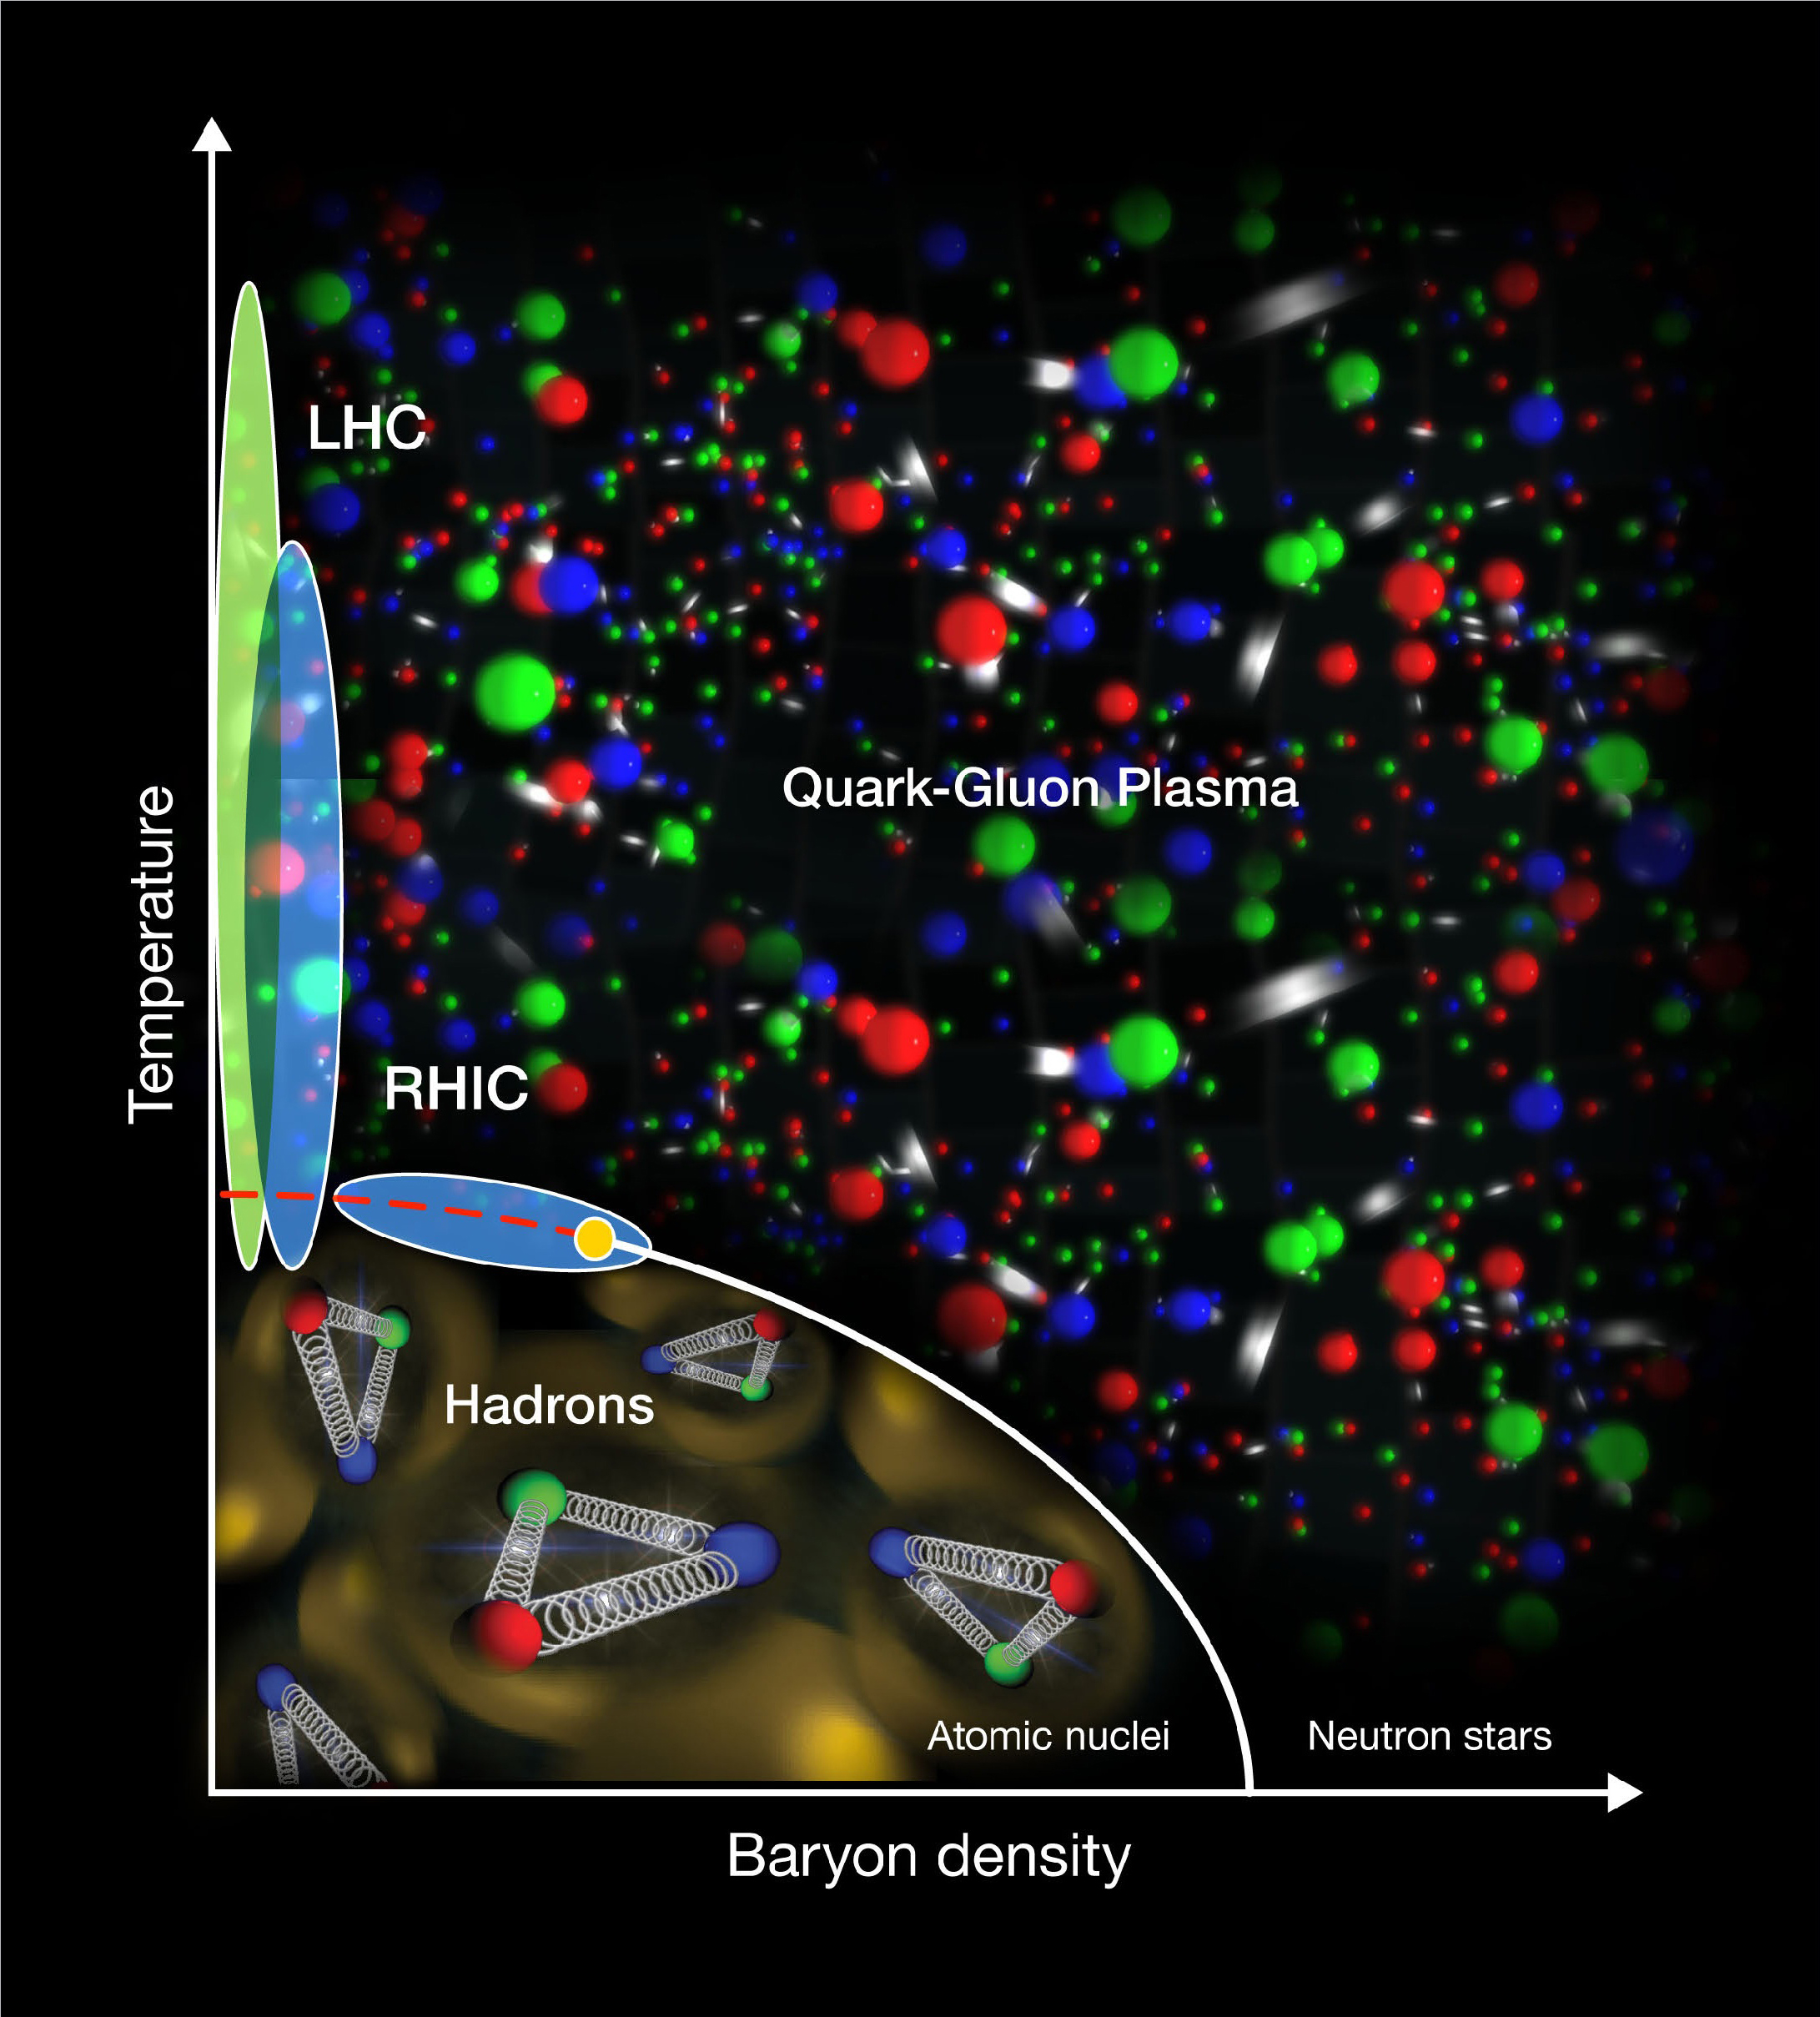
\includegraphics[width=10.0cm]{figures/RHIC_Graphics_Fig1-HR}}
\caption{A schematic phase diagram of QCD matter \cite{fig_phase_dia}}
\label{fig1}
\end{figure}



\section{Heavy ion collision}

As mentioned above, the universe started from a single point at approximately 14 billion years ago~(Big Bang), and expanded and cooled down. During this expansion, the transition from a QGP phase to a hadronic phase happened which allowed for the formation of hadrons.  To study this procedures, we collide heavy-ions at ultra-relativistic energies, where one creates QGP matter in the laboratory under controlled conditions. 

In the LHC experiment, the heavy ions are accelerated up to almost the speed of light and collide with each other. In this relativistic heavy ion collision, the initial energy density participating in the collision is expected to be well above the threshold for the QGP formation \cite{PhysRevD.27.140}.  In a canonical picture of the collision \cite{Kolb:2003dz} the system evolution can be divided into several stages, as shown in Fig.\ref{fig2}
  \begin{enumerate}
 	\item Initial state
 	\item thermalized QGP
 	\item hadronic gas
 	\item chemical freeze-out
 	\item kinetic freeze-out(free streaming)
 \end{enumerate}
 
 	At first, the two nuclei traveling at relativistic speeds become longitudinal Lorentz-contracted disks. A large number of the collisions between participants in target and projectile nuclei occur, and it is expected that the produced partons are strongly coupled with each other and thermalized into the QGP phase rapidly within a short time (less than a few fm/$c$). After $\sim 20$fm/$c$ the temperature of the expanding medium drops down below the critical temperature $T_c$ \cite{Rapp2011}. The quarks and gluons become confined into hadrons.  Afterward, the expansion (and the temperature fall) leads to a reduction of the inelastic processes among hadrons, until the relative abundance of hadron species is fixed (chemical freeze-out), and then to the stop of any interaction which fixes the kinetic spectra (kinetic freeze-out).
 	
 
\begin{figure}[h]
\centerline{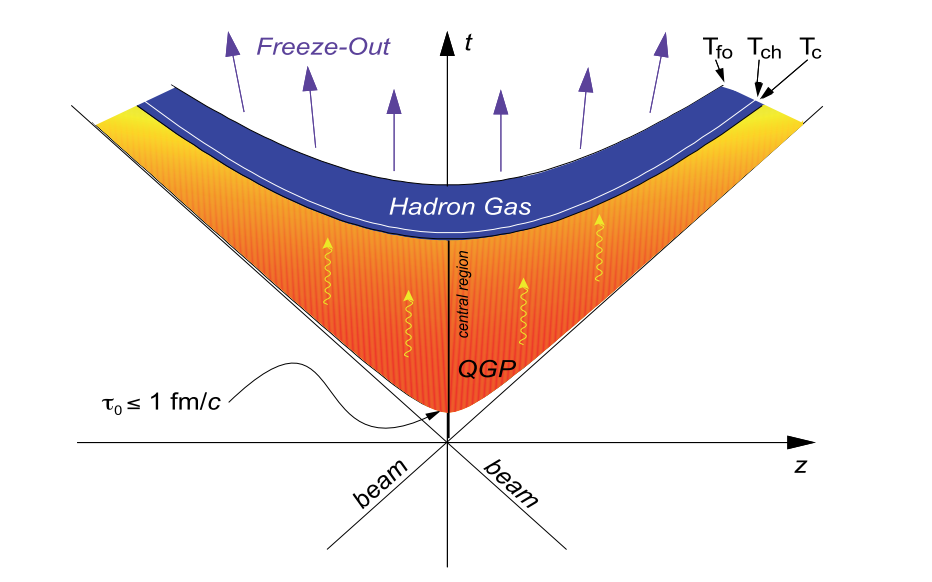
\includegraphics[width=13.0cm]{figures/system_evol}}
\caption{Schematic light cone diagram of the evolution of a high energy
heavy ion collision}
\label{fig2}
\end{figure}

	To verify the existence of the phase transition and the formation of QGP in heavy ion collisions, physics observables should be identified for each stage of dynamical evolution of the produced medium. Ordered in sequence of their formation in the course of the dynamics, the most relevant observables are characterized as follows:
	
	\begin{itemize}
		\item Suppression of heavy quarkonia production by Devye screening in the QGP
		\item Suppression of di-jets by losing their energy in the medium, so the undisturbed parton form a jet while the other one is absorbed in the medium and not detected (or distorted)
		\item High-$p_T$ particles produced in primordial $\hat{q}q, \hat{g}g, \hat{q}q$ reactions with high momentum transfer are attenuated by gluonic bremsstrahlung in QGP medium
		\item Hydrodanamics collective motion develops with the onset of thermal equilbrium
		\item Hadronic chemical freeze-out fixes the abundance ratios of the species
		\item Two particle Bose-Einstein-Correlations (the HBT effect of quantum optics) resulted from the kinetic freeze out stage
	\end{itemize}


 	Notably, the QGP matter collectively expand both in the longitudinal and the transverse direction. The transverse expansion leads the collectivity motion of system, which is often called the flow. The produced particles gain the momentum and energy from the radial flow of the QGP matter, and a final distribution of the transverse momentum is modified from the superposition of the independent nucleon-nucleon collisions \cite{Shen:2011eg}.
 	


\section{Flow}
\label{sec:flow}
\subsubsection{Introduction}
  In previous section, the phase transition is expected to occur at $T_c \sim 150$~MeV, corresponding to an energy density of $\epsilon_c \simeq 0.15 - 0.5$~GeV/$fm^3$ \cite{Bazavov:2014pvz}, which could be already be achieved at RHIC or LHC energies. Thus, experimental measurements in relativistic heavy ion collisions could shed light on the properties of the QGP. The main goal of studying relativistic heavy ion collisions is to discover and understand its properties of created matter. The system produced in relativistic heavy ion collisions dynamically evolves within a time duration of the order of fm/$c$. Therefore one has to describe the space-time evolution of thermodynamic variables to fill the large gap between the static aspects of QGP properties and the dynamical aspects of heavy ion collisions, and hydrodynamics plays an important role in connecting them. Hydrodynamics is thus applied to matter under local equilibrium in the intermediate stage.

Also by using hydrodynamics, we can remove QCD Lagrangian density

\begin{equation}
	\mathcal{L} = \bar{\psi_i}(i\gamma_\mu D^{\mu}_{ij} - m \delta_{ij})\psi_j - \frac{1}{4}F_{\mu v \alpha}F^{\mu v \alpha} 
\end{equation}
\smallskip

	where $\psi_i$ is a quark field, $\gamma$ are Dirac matrices, $D$ is a covariant derivative, $m$ is a quark mass, $\delta$ is the Kronecker delta symbol, and $F$ is the field strength of the gluons. In spite of simple looking of QCD Lagrangian form, it is very difficult to make any predictions directly from QCD due to its complexity which mainly arises from the non-linearity of the interactions of the gluons, the strong coupling, the dynamical many body system and confinement. In hydrodynamics, however, as a phenomenological theory, we can express the equation of state as follows: 
	
	\begin{equation}
		P = P(e, n)
	\end{equation}
	\smallskip 
	
	which expresses the pressure $P$ as a function of energy density $e$ and the baryon density $n$. Such an equation can be obtained by performing numerical simulations of QCD on the lattice. To calculate the above equation of the states, it is also necessary to use additional transport coefficients such as shear viscosity $\eta$, bulk viscosity $\zeta$, heat conductivity $\lambda$, etc. 
	
	%check it one more time
	Hydrodynamics can also produce outputs, such as local temperature or energy density, that could be useful in describing the dynamics for other observables. For instance, in the current formalism of jet quenching, one needs information regarding parton density or energy density along a trajectory of an energetic parton.
	
  Hydrodynamics also provides information regarding bulk matter. Therefore we can say that, in the context of relativistic heavy ion collisions, hydrodynamics is the heart of the dynamical modeling since it not only describes expansion and collective flow of matter, but also provides important information about the intermediate stage for other phenomena.
	
	\subsubsection{Formal definitions}
	The particle azimuthal distribution($r(\varphi$)) is a periodic quantity (over 0 to $2\pi$ in polar coordinate), and it can be expand with customary expressed in a Fourier series \cite{Voloshin:2008dg, Voloshin1996},
	
\begin{equation}
	r(\varphi)=\frac{x_0}{2\pi} + \frac{1}{\pi}\sum_{n=1}^{\infty}[x_n \cos(n\varphi) + y_n \sin(n\varphi)]
	\label{eq:flow}
\end{equation}
\smallskip
	
	
	where, Fourier coefficient $x_n, y_n$ is defined as
	
\begin{equation}
	x_n = \int_{0}^{2\pi} r(\varphi)\cos(n\varphi)d\varphi	
\end{equation}
\begin{equation}
	y_n = \int_{0}^{2\pi} r(\varphi)\sin(n\varphi)d\varphi	
\end{equation}
\smallskip

For our case, the multiplicity is finite, therefore $x_n$ and $y_n$ are changed into finite sum as like

\begin{equation}
x_n=\sum_{\nu}r_{\nu}\cos{n\phi_{\nu}}
\end{equation}
\begin{equation}
y_n=\sum_{\nu}r_{\nu}\sin{n\phi_{\nu}}
\label{eq:yndef}
\end{equation}
\smallskip

 $r_\nu$ is weight for particle, and usually it takes unity($r_v = 1$) for inclusive flow measurement. If there is no flow effect and fluctuation, the azimuthal distribution $r(\varphi)$ should be const. i.e. isotropic multiplicity for all angles, and all the coefficient of $\sin$ and $\cos$ terms will be vanished. On the other hand, if there are any anisotropic effect, coefficient $x_n$ and $y_n$ will survive. 
 
 If we define the $v_n$, and $\psi_n$ for each corresponding Fourier's harmonics in the following way:

\begin{equation}
	v_n \equiv \sqrt{x_n^2 + y_n^2}
\end{equation}
\begin{equation}
	0 \le \psi_n \le \frac{2\pi}{n} 
\end{equation}
\smallskip

we can now express azimuthal particle distribution with $v_n$ and $\psi_n$ instead of $x_n$ and $y_n$.

\begin{equation}
x_n=v_n \cos{n\psi_n}
\end{equation}
\begin{equation}
y_n=v_n \sin{n\psi_n}
\label{eq:xnyndef}
\end{equation}
\smallskip

If we put back $x_n$ and $y_n$ into original Eq.\ref{eq:flow}  then

\begin{equation}
\frac{dN}{d\phi}=\frac{x_0}{2\pi}+\frac{1}{\pi}\sum_{n=1}{(v_n\cos{n\psi_n}\cos{n\phi}+v_n\sin{n\psi_n}\sin{n\phi})}
\label{eq:flow_sinterm}
\end{equation}

\begin{equation}
=\frac{x_0}{2\pi}+\frac{1}{2\pi}\sum_{n=1}{(2v_n\cos{n(\phi-\psi_n)})}
\label{eq:flow_final}
\end{equation}
\smallskip


From Eq.\ref{eq:flow_sinterm} to \ref{eq:flow_final}, the sinus terms were vanished because of symmetry of the collision. As illustrated in Fig.\ref{fig3}, if the colliding nuclei are the same, the probability for a produced particles to be emitted in direction $\varphi$ and $-\varphi$ is equal. As defined in Eq.\ref{eq:yndef}, $y_n$ is average of $\langle \sin(n\varphi) \rangle$, and this average of sinus term will be canceled each other of any angle $\varphi$ with its symmetries
\begin{equation}
	\sin(n\varphi) + \sin(n(-\varphi)) = \sin(n\varphi) - \sin(n\varphi) =0
\end{equation}

From Eq.\ref{eq:flow_final}, harmonics $v_n$ can be related explicitly to the origin azimuthal distribution $r(\varphi)$ in the following way:

\begin{eqnarray}
	\langle \cos(n\varphi) \rangle &\equiv& \frac{\int_{0}^{2\pi}{\cos(n\varphi)r(\varphi)d\varphi}}{\int_0^{2\pi}{r(\varphi)d\varphi}} \\
	&=&\frac{\frac{1}{\pi} v_n \int_{0}^{2\pi}{\cos^2(n\varphi)d\varphi}}{v_0} \\ 
	&=& \frac{v_n}{v_0}
	\label{eq:vncal}
\end{eqnarray}

Using a normalized distribution $r( \varphi )$, for which $v_0 = \int_{0}^{2\pi}{r ( \varphi )} d\varphi = 1$, the above equation leads to:
	
\begin{equation}
	v_n = \langle \cos(n\varphi) \rangle 	
\end{equation}
\smallskip


	The harmonic $v_1$ is often called ``directed flow", and $v_2$ called ``elliptic flow", and $v_3$ is ``triangular flow". When we consider the polar coordinate with $(r, \varphi)$, then the distribution for eillipse-like is determined by the following equation. 
	

\begin{equation}
	r(\varphi) = \frac{a(1-\varepsilon^2)}{1+\varepsilon \cos \varphi}
\end{equation}
\smallskip

	where $\varepsilon$ is the eccentricity defined as 
\begin{equation}
	\varepsilon^2 \equiv 1 - \frac{b^2}{a^2}
\end{equation}

	with definition of a is major, and b is minor axis. With this parameterization, $v_n$ can be calculated analytically in a closed form, as like
\begin{equation}
	v_n = 2\pi b(-1)^{n}(\frac{a-b}{a+b})^{\frac{n}{2}}
\end{equation}

	The methods that attempt to explain the azimuthal distribution of particles produced with customized Fourier's expansion have been succeeded in relativistic heavy ion collision, especially in RHIC and LHC, by studying about strong collective and anisotropic flow in the transverse plane driven by the pressure gradients with more particles emitted in the direction of the largest gradients. The large elliptic flow discovered at RHIC energies \cite{Ackermann:2000tr} continuous to increase also in LHC energies \cite{Aamodt:2010pa,Adam:2016izf}. This has been predicted by calculations utilizing viscous hydrodynamics \cite{Romatschke:2007mq,Shen:2011eg,Schenke:2011zz,Bozek:2012qs,Gale:2012rq,Hirano:2010je}.

These calculations also demonstrated that the shear viscosity to the entropy density ratio ($\eta/s$) of strongly interacting matter is close to a universal lower bound $1/4\pi$ \cite{Kovtun:2004de} in heavy ion collisions at RHIC and LHC energies.

%The magnitude of the anisotropic flow has been to found to be sensitive to the transport properties, as well as the space-momentum profile in the initial state~\cite{}. 
The temperature dependence of the $\eta/s$ has some generic features that most of the known fluids obey. One such general behavior is that the ratio typically reaches its minimum value close to the phase transition region \cite{Lacey:2006bc}. 
It was shown, using kinetic theory and quantum mechanical considerations \cite{PhysRevD.31.53} that $\eta/s>1/15$ would be an order of magnitude for the lowest possible shear viscosity to entropy ratio in nature. Later it was found that one can calculate an exact lower bound $(\eta/s)_{\rm min}=1/4\pi\approx0.08$ using the AdS/CFT correspondence \cite{Kovtun:2004de}. Hydrodynamical simulations supports as well the view that the QGP matter indeed is close to that limit \cite{Gale:2012rq}. 	
	
	 In relativistic collision, each collision is characterized by the impact parameter, defined as the distance between the center of two nuclei points. Collisions with the short impact parameter are called central collisions and collisions with the long impact parameter are called peripheral collisions.  This geometry of the collision moments with non-central collision has ellipticity in the transverse plane and is shown in Fig.\ref{fig3}
	
\begin{figure}[t]
\centerline{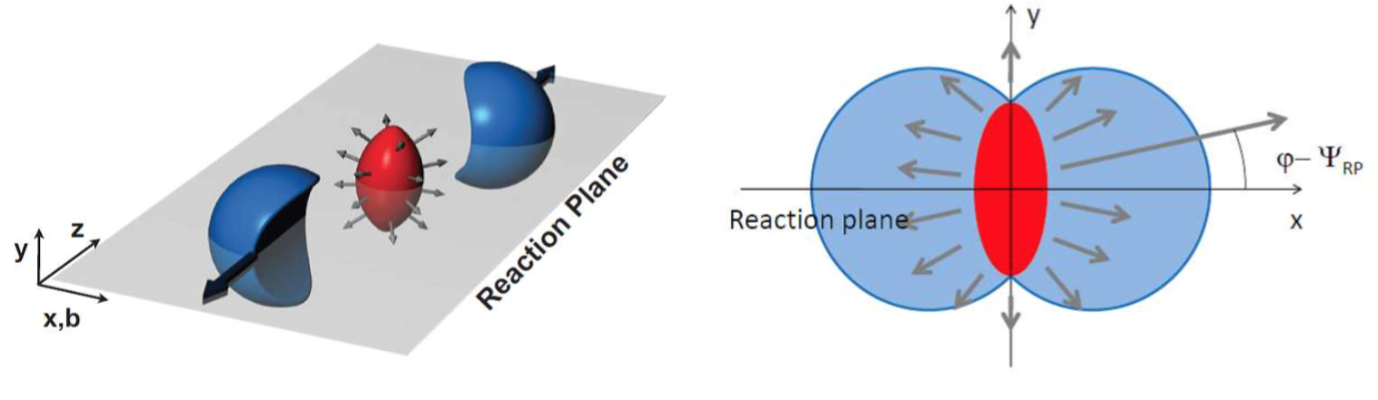
\includegraphics[width=13.0cm]{figures/flow_clasic}}
\caption{Schematic sketch of transverse projectile view of the non-central collision \cite{Snellings:2011sz}. The matter created in the collision (red) is called the participant region. The nucleons in the blue region are called spectators. The grey plane in the left figure is called the reaction plane.}
\label{fig3}
\end{figure}

	The initial spatial anisotropy in the azimuthal direction is transformed to the anisotropy of the final particle momentum distributions due to the collective expansion of the produced system. During evolution of the almond-shaped interaction volume, the anisotropy in coordinate space is transformed to anisotropy in momentum space (shown in Fig.\ref{fig4}). Therefore, these momentum anisotropies of the hydrodynamic matter lead to the anisotropic azimuthal distribution of the produced particles. 
	
	However, the transverse expansion of system volume is insufficient to explain the anisotropy of azimuthal particle distribution. As shown in Fig.\ref{fig5}, if there is no interaction between particles (or the mean free path among the produced particles is much longer than the typical size of the system), the azimuthal distribution of the particles does not depend on azimuthal angle on average due to symmetry of the production process. On the other hand, when the mean free path is very small compared to the typical system size, hydrodynamics can be applied to describe the space-time evolution of the system. Furthermore, the pressure gradient along the horizontal axis is much longer than the vertical axis due to the geometry.
 

 	
\begin{figure}[t]
\centerline{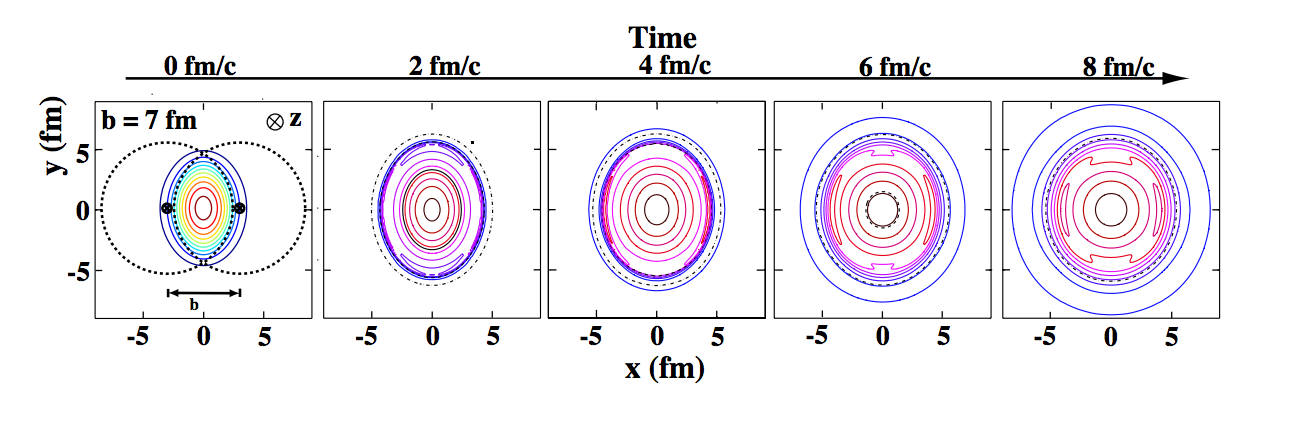
\includegraphics[width=12.0cm]{figures/system_time_flow}}
\centerline{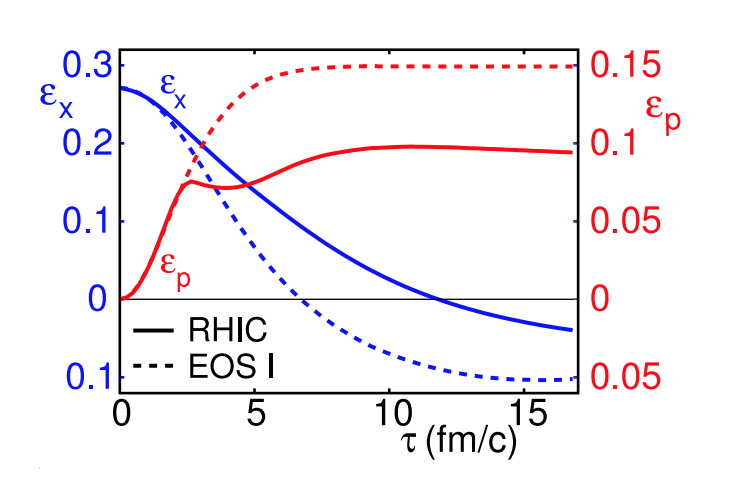
\includegraphics[width=9.0cm]{figures/time_ecenx_ecenp}}
\caption{The created initial transverse energy density profile and its time
dependence in coordinate space for a non-central heavy-ion collision \cite{Kolb:2003dz} As shown in the bottom figure, the anisotropy of space($\epsilon_x$) coordinate becomes smaller over time, while the momentum anisotropy of momentum space ($\epsilon_p$) increases as system expand as time goes. }
\label{fig4}
\end{figure}


	The origin of large $v_2$ cannot explain other harmonics especially odd number harmonics like $v_3$, $v_5$, etc. The impact parameter vector b (the vector connecting the centers of two colliding nucler) changes event-by-event, which in turn yields a random reaction plane angle $\psi_R$ (the plane spanned by the impact parameter and the beam axis). Due to these random fluctuations, it is not trivial to set up for each event the coordinate system. Because of the random geometry of participant nucleon in colliding nuclei, the overlap region shape is not a perfect almond shape, but rather a complex shape as shown in Fig.\ref{fig:complexshape}. As a result of this random fluctuation and the complex shape of the energy density profile of the system, the flow harmonics $v_n$ are defined with their own event plane $\psi_n$, not with respect to reaction plane $\psi_R$. Although the 2nd harmonics symmetry plane($\psi_2$) roughly corresponds to the reaction plane($\psi_2 \sim \psi_R)$, their azimuthal angles are slightly inclined event-by-event. In the following section, methods to calculate flow will be discussed.
		

\begin{figure}[h]
\centerline{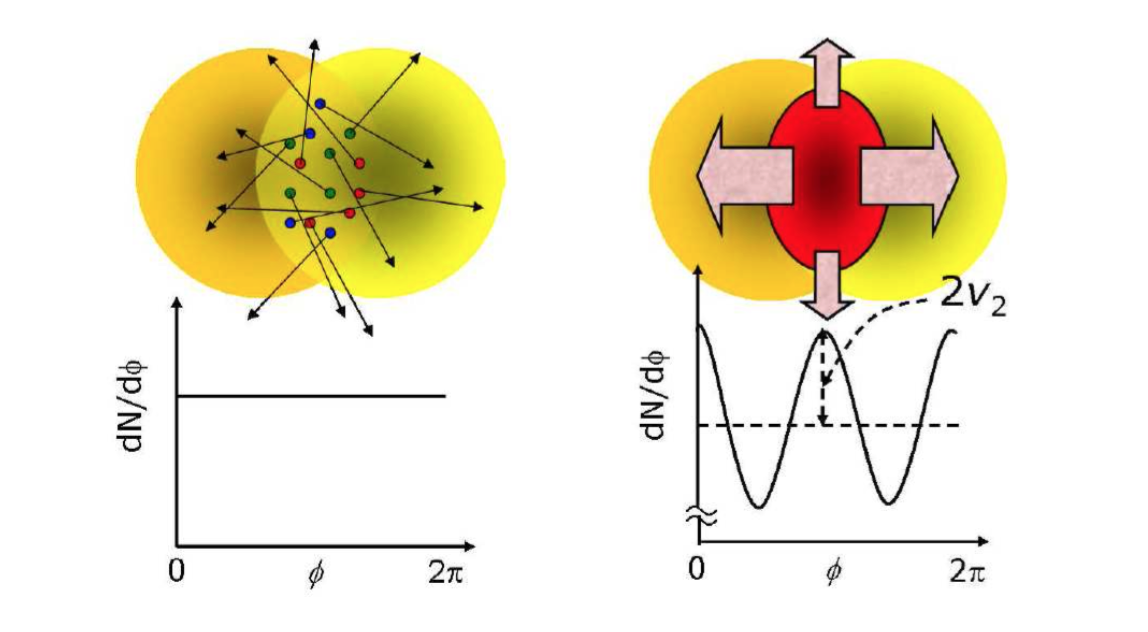
\includegraphics[width=13.0cm]{figures/v2explin}}
\caption{The illustration of the elliptic flow development in the two extreme cases: a large and small mean free path among the produced particles in the left and right images, respectively \cite{Voloshin:2008dg}.}
\label{fig5}
\end{figure}

\begin{figure}[h]
\centerline{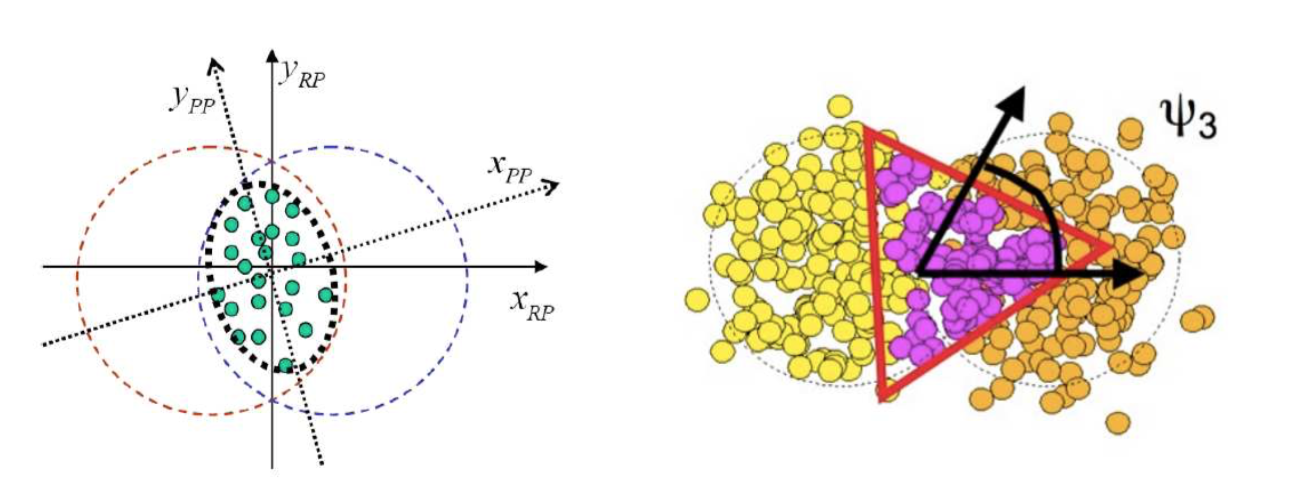
\includegraphics[width=13.0cm]{figures/fig_complxshape}}
\caption{The transverse profile in a single event simulated using the Monte Carlo Glauber model \cite{Miller:2007ri, Bzdak:2006qk}. (left) Green circles are the positions of the nucleon-nucleon collisions. The 2nd harmonic event plane is slightly inclined around the reaction plane. (right) It also has a non-zero triangle anisotropy. The azimuthal angle of the triangle anisotropy, i.e., the 3rd event plane angle $\Psi_3$ is not correlated to the reaction plane}
\label{fig:complexshape}
\end{figure}



\subsection{Event Plane method}

The event plane method (EP) is the most commonly used method to measure anisotropic flow. Using this method, the event plane is estimated and all particles' azimuthal angles are correlated to this estimated plane in order to obtain the flow harmonics $v_n$. From the Eq.\ref{eq:xnyndef} we can easily calculate event plane angles with the following way:


\begin{equation}
\frac{y_n}{x_n}=\frac{v_n\sin{n\psi_n}}{v_n\cos{n\psi_n}}=\tan{n\psi_n}
\end{equation}
\begin{equation}
\psi_n=(\arctan{\frac{y_n}{x_n}})/n
\end{equation}


and by using Fourier's coefficient relation:

\begin{equation}
v_n=\langle\cos{n(\phi_\nu - \psi_n)}\rangle 
\label{vndef}
\end{equation}
\smallskip


However, in practice, since each event has a finite number of created particles, the results for the event plane angle will be affected by a limited resolution. This can be corrected for by estimating the event plane resolution:

\begin{equation}
v_n^{measured}=\langle\cos{n({\phi-\psi_n^{measured})}}\rangle
\end{equation}
\smallskip

where, $\psi_n^{measured} = \psi_n + \psi_n^{err}$

\begin{eqnarray}
v_n^{measured}&=&\langle\cos{n(\phi-\psi_n-\psi_n^{err})}\rangle \\
&=&\langle\cos{n(\phi-\psi_n)}\cos{n(\psi_n^{err}})+\sin{n(\phi-\psi_n)}\sin{n(\psi_n^{err})}\rangle \\
&=&\langle\cos{n(\phi-\psi_n)}\cos{n(\psi_n^{err}})\rangle+\langle\sin{n(\phi-\psi_n)}\sin{n(\psi_n^{err})}\rangle \\
&=&\langle\cos{n(\phi-\psi_n)}\rangle\langle\cos{n(\psi_n^{err}})\rangle \\
&=&v_n\langle\cos{n(\psi_n^{err})}\rangle
\end{eqnarray}

Finally, we get 

\begin {equation}
v_n = v_n^{measured}/\langle\cos{n(\psi_n^{err})}\rangle
\end {equation}
\smallskip


We assume that event angle error($\psi_n^{err}$) is independent of $\phi-\psi_n$, and the expectation value of $\sin{n(\psi_n^{err})}$ is zero. The estimated event plane resolution can be obtained by two or more independent subevents \cite{PhysRevC.58.1671}. The advantage of the event plane method is that it is less sensitive to the number of particles for analysis, and can therefore be used to measure flow of rare particles. Furthermore, this method can be used to estimate an event plane, especially the 2nd order event plane which is expected to be similar to the reaction plane $\psi_2 \sim \psi_R$. This 2nd event plane also can be used for jet or other analysis. The main disadvantage of this method occurs when the event plane resolution is affected by correlations which do not stem from a genuine correlation of all particles with the true event plane. While event plane resolution can fix errors from multiplicity, it cannot fix errors originating from non-flow (e.g., jet, detector smearing, etc.). 

\subsection{Scalar product method}

	The original idea behind the event plane method is that the direction of $\Psi_n$ of the flow vector in a reference frame provides an estimation of the corresponding angle $\Phi_n$ in the underlying probability distribution. Because a finite sample of particles is used, statistical fluctuation causes $\Psi_n$ to differ from $\Phi_n$. This dispersion is characterized by the ``resolution", defined as
	
	\begin{eqnarray}
		R &\equiv & \langle e^{in(\Psi_n - \Phi_n} \rangle  \\
			&=& \left\langle \frac{Q_n}{|Q_n|} e^{-in\Phi_n} \right\rangle 
	\end{eqnarray}

	For the fixed $v_n$, the above equation can be written in the form of
	
	\begin{eqnarray}
		R(v_n) &\equiv &  \left\langle e^{in(\Psi_n - \Phi_n)} \right\rangle _{|vn} \\ 
		&=& \left\langle \frac{Q_n}{|Q_n|} e^{-in\Phi_n} \right\rangle _{|vn} \label{eq:res_def}
	\end{eqnarray}
	
	where $\langle ... \rangle _{|vn}$ indicates an average over a large number of event with the same underlying $v_n$. From the Eq.\ref{vndef}, we can see underlying probability distribution (Eq.\ref{eq:flow}) depends on the relative magnitude of the anisotropy $v_n$ to the statistical dispersion $1/\sqrt{N}$. In the limit $v_n \gg 1/\sqrt{N}$ (large number of multiplicity), easily reconstruct the underlying event plane so that $\Phi_n = \Psi_n$,(i.e. $R(v_n) \sim 1$, and conversely, when the $v_n \sqrt{N} \ll 1$ (low multiplicity) the Resolution $R(v_n) \sim kv_n$, where k is independent of $v_n$ and scale as $k \sim \sqrt{N}$. 
	
	%%% change this
	Generally, the value falls somewhere between these limits \cite{Luzum:2013yya}, and this nonlinear dependence of the resolution on the underlying flow is the origin of the difficulties of the event plane method.
	
	When we obtain the event plane resolution from subevents A and B, the resolution $R(v_n)$ is a factorization like the below  definition:
	
	\begin{eqnarray}
		\left \langle \frac{Q_{nA}}{|Q_{nA}|}  \frac{Q_{nB}}{|Q_{nB}|} \right \rangle &=&  \left \langle \frac{Q_{nA}}{|Q_{nA}|} e^{-in\Phi_n} \right \rangle \left \langle \frac{Q_{nB}}{|Q_{nB}|} e^{-in\Phi_n} \right \rangle^{*} \\
		&=& \left |   \left \langle   \frac{Q_{nA}}{|Q_{nA}|} e^{-in\Phi_n}  \right \rangle _{|v_n} \right | ^{2} \\ 
		&=&  R(v_{nA})^2
	\end{eqnarray}
	The Eq.\ref{eq:res_def} is used for the second line to third line of the above equation. The event-plane methods is thus defined as:
	
	\begin{equation}
		v_n\{EP\} \equiv \frac{\left \langle Q_n \frac{Q_{nA}^*}{|Q_{nA}|} \right \rangle }{\sqrt{\left \langle  \frac{Q_{nA}}{|Q_{nA}|}  \frac{Q_{nB}}{|Q_{nB}|} \right \rangle }}
		\label{eq:EP}
	\end{equation}
	\smallskip
	
	Since the measurement has been taken with the average of all events in a given centrality class, Eq.\ref{eq:EP} changes as term of $v_n$ as like
	
	\begin{equation}
		v_n\{EP\} = \frac{\langle v_n R(v_{nA})\rangle _{v_n}}{\sqrt{\langle R(v_{nA})^2 \rangle _{v_n} }}
	\end{equation}
	\smallskip 
	
	Note that $\langle R(v_{nA})^2 \rangle \neq \langle R(v_{nA})\rangle ^2$. Resolution correction is no longer a simple projection of the measured event plane $\Psi_n$ onto the ``true" event plane $\Phi_n$.
	
	In the limit of infinite multiplicity (i.e. $R(v_n) \sim 1$), $v_n\{EP\}$ does indeed measure the event averaged mean $v_n$ from Eq.\ref{eq:flow}. But in reality, the resolution is not perfect and the result is usually even closer to the low resolution limit \cite{Alver:2008zza}, and in this case, the event-plane measurement thus yields a root-mean-square value. In other words, what we measure with the event plane method is some values between root-mean-square and mean of $v_n$ depends on the resolution (i.e. Event multiplicity or the performance and acceptance of detector)
	
	\begin{equation}
		v_n\{EP\} \simeq \langle v_n \rangle \quad \text{(high resolution limit)}
	\end{equation}

	\begin{equation}
		v_n\{EP\} \simeq \sqrt{\langle v_n^2 \rangle}  \quad \text{(low resolution limit)}
	\end{equation}
	\smallskip
	
	However, in the scalar product method, which is a slight variant of the event plane method, consists of removing the factor of $|Q_n|$ before taking the average in the numerator and denominator of Eq.\ref{eq:EP}
	
	
	\begin{equation}
		v_n\{SP\} \equiv \frac{\langle Q_n Q_{nA}^*\rangle}{\sqrt{\langle Q_n Q_{nA}^*\rangle}}
	\end{equation}
	\smallskip 
	
		Then, by calculating the scalar product in numerator, the fluctuation term (Resolution related terms) are removed. 
		
	\begin{equation}
		v_n\{SP\} = \frac{\langle v_n v_{nA} \rangle _{v_n} }{\sqrt{\langle v_n v_{nA} \rangle _{v_n}}} = \sqrt{\langle v_n^2 \rangle }
	\end{equation}	
	\smallskip
	
	As a result, the scalar product method always yields the root-mean-square $v_n$, regardless of the details of the analysis and makes for a superior measurement. 
	
\subsection{Cumulants method}

\subsubsection{Multi particle correlations}

Because of the disadvantage of the event plane method (or the scalar product method) in estimating the event plane, the cumulants method (often called the multi-particle correlation method) was proposed in order to reduce this bias. This method does not require the event plane estimation event-by-event. Instead, these multi-particle correlations can be calculated by looping over all possible multiplets. If we assume that all the particles have azimuthal correlations which originated from flow harmonics only, then 2- and 4- particle azimuthal correlations can be expressed in the following way:
	
\begin{equation}
	\langle 2 \rangle \equiv  \langle e^{in(\phi_1 - \phi_2)} \rangle \equiv \frac{1}{{M \choose 2}2!}\sum_{i,j=1, i\neq j}^{M}{e^{in(\phi_i - \phi_j)}}
\end{equation}
\begin{equation}
	\langle 4 \rangle \equiv \langle e^{in(\phi_1 + \phi_2 - \phi_3 - \phi_4} \rangle \equiv \frac{1}{{M \choose 4}4!}\sum^{M}_{i\neq j\neq k \neq l}e^{in(\phi_i + \phi_j - \phi_k - \phi_l)}
\end{equation}
\smallskip

where the brackets denote the particle average in a single event. The $i, j, k, l$ denote identical particles, and $\phi_i$ is the azimuthal angle of the $i$-th particle measured in laboratory frame. To prevent contribution of self(auto) correlation, the constraints $i \neq j$ and $i \neq j \neq k \neq l$ have been enforced. When we extend the above equation for event average, then 2- and 4- particle azimuthal correlations are as follows :

\begin{equation}
	\langle \langle 2 \rangle \rangle \equiv \langle \langle e^{in(\phi_1 - \phi2)} \rangle \rangle \equiv \frac{\sum_{i=1}^{N}{(W_{\langle 2 \rangle})_i}\langle 2 \rangle_2 }{\sum_{i=1}^{N}{(W_{\langle 2 \rangle})_i}}
\end{equation}
\begin{equation}
	\langle \langle 4 \rangle \rangle \equiv \langle \langle e^{in(\phi_1 + \phi_2 - \phi_3 - \phi_4)} \rangle \equiv \frac{\sum_{i=1}^{N}{(W_{\langle 4 \rangle })_i}\langle 4 \rangle_i }{\sum_{i=1}^{N}{(W_{\langle 4 \rangle})_i}}
\end{equation}
\smallskip

where, N is the number of events, and $W_{\langle 2 \rangle}$ and $W_{\langle 4 \rangle}$ are the event weights. The selecting event weight is explained in Appendix B. The benefit of using multi-particle azimuthal correlation is to measure flow harmonics $v_n$ without requiring the event plane $\psi_n$, 

\begin{eqnarray}
	\langle \langle 2 \rangle \rangle \equiv \langle \langle e^{in(\phi_1 - \phi_2)} \rangle  \rangle &=& \langle \langle e^{in(\phi_1 - \psi_n - \phi_2 + \psi_n)} \rangle \rangle  \\
		&=& \langle \langle e^{in(\phi_1 - \psi_n)} \rangle \langle e^{-in(\phi_2-\psi_n)} \rangle \rangle = \langle v_n^2 \rangle
		\label{eq:vn2}
\end{eqnarray}

In cases when only flow correlations exist in the system, the correlation among any two particles is induced through the correlation of each particle with the same event plane $\psi_n$ \cite{Wang:1991qh, Tsang:1991zza}.
Each of these single particle azimuthal distributions is related to the flow harmonics via Eq.\ref{eq:flow_final}. Therefore we can show that :

\begin{equation}
	\langle \langle 4 \rangle \rangle = \langle v_n^4 \rangle 
\label{eq:vn4}
\end{equation}
\begin{equation}
	\langle \langle 6 \rangle \rangle = \langle v_n^6 \rangle 
\label{eq:vn6}
\end{equation}
\begin{equation}
	\langle \langle 8 \rangle \rangle = \langle v_n^8 \rangle
\label{eq:vn8}
\end{equation}


and so on, in a similar manner. Crucially, even in an ideal case when there is an absence of non-flow effects, the cumulants method will be systematically biased due to flow fluctuation. 

\begin{equation}
	\langle v_n \rangle^k \neq \langle v_n^k \rangle
\end{equation}
\smallskip

\subsubsection{Flow fluctuation}	

	%check it again
The measuring of flow harmonics is paramount to the measuring of the power of average values of flow harmonics with multi-particle correlation. However, these two values are not exactly equivalent even in the ideal case, i.e., when there is no non-flow effect scenario due to unavoidable flow fluctuations. In the following section methods for quantifying various powers of flow harmonics will be discussed. For better convention, $v_n$ will be denoted as simply $v$.

First, let's consider the Taylor expansion for arbitrary functions around mean $\mu_x $ up to second order

\begin{equation}
	h(x) = h(\mu_x) + (x-\mu_x)h'(\mu_x)+\frac{(x-\mu_x)^2}{2!}h''(\mu_x)
\end{equation}
\smallskip

If we take the average of given function $h(x)$ then the Taylor expansion can be expressed as:

\begin{eqnarray}
	\langle h(x) \rangle &=& h(\mu_x) + ( \langle x \rangle - \mu_x )h'(\mu_x) + \frac{\sigma_x^2}{2}h''(\mu_x)  \\
	&=&  h(\mu_x) + ( \mu_x- \mu_x) h'(\mu_x) + \frac{\sigma_x^2}{2}h''(\mu_x) \\ 
	&=& h(\mu_x) +\frac{\sigma_x^2}{2}h''(\mu_x) 	\label{eqn:taylor}
\end{eqnarray} 
	
	where,
	
	$$ \sigma_x^2 = \int_{-\infty}^{\infty} (x-\mu_x)f(x)dx $$
	\smallskip
	
As seen in this equation, the expectation value of linear term(first order) in Taylor's expansion of $h(x)$ around mean $\mu_x$ always vanishes. Then we can now estimate the average of various powers of $v$ from Eq.\ref{eq:taylor}. For example, in the case $h(v)=v^2$, it follows that :

\begin{equation}
	\langle v^2 \rangle = \langle v \rangle^2 + \sigma_v^2 
\end{equation}

By using the definition of multi- particle correlation (Eq.\ref{eq:vn2} to \ref{eq:vn8}), we have 

\begin{equation}
	v\{2\} = \langle v^2 \rangle ^{1/2}
\end{equation}

Furthermore, by applying the Taylor expansion above (Eq.\ref{eqn:taylor}) for the case $h(v) \equiv v^2$, it follows that:

\begin{eqnarray}
		\langle v^2 \rangle &=& (\langle v \rangle^2 + \sigma_v^2)^{1/2} \\
		&=& \langle v \rangle \left( 1+\frac{\sigma_v^2}{\langle v \rangle^2} \right)^{1/2} \\ 
		&\simeq & \langle v \rangle \left( 1+\frac{1}{2} \frac{\sigma_v^2}{\langle v \rangle^2} \right) 
\end{eqnarray}

For the constraint with:
\begin{equation}
	\sigma_v \ll \langle v \rangle
\end{equation}

Then we have general results:

\begin{equation}
	(1+x)^n \simeq 1 + nx,
\end{equation}
valid for $x \simeq 0$, and the final equation can be expressed as like

\begin{equation}
	v\{2\} \simeq \langle v \rangle + \frac{1}{2} \frac{\sigma_v^2}{\langle v \rangle}
	\label{eq:2p-cumulant}
\end{equation}

From this result, we can conclude that the flow estimation with the 2nd order cumulant will be always systematically biased with positive signature due to flow fluctuations.

In addition, the four-particle cumulant can be defined similarly. From the definitions

\begin{equation}
	v\{4\} = ( -\langle v^4 \rangle + 2\langle v^2 \rangle ^2 )^{1/4}
\end{equation}

with Talyer expansion (Eq.\ref{eqn:taylor}) for the case $h(v) \equiv v^4$ we have up to second order in $\sigma_v$ as

\begin{equation}
	\langle v^4 \rangle = \langle v \rangle^4 + 6\sigma_v^2\langle v \rangle ^2 
\end{equation}

as same as 2-particle cumulants, it follows that:

\begin{eqnarray}
	v\{4\} &=& \left[ -\left\langle v \right\rangle^4 - 6 \sigma_v^2 \langle v \rangle^2 + 2\left( \langle v \rangle^2 + \sigma_v^2 \right)^2 \right]^{1/4} \\
	&=& \left[ \langle v \rangle^4 - 2 \sigma_v^2 \langle v \rangle ^2 + \mathcal{O}(\sigma_v^4) \right]^{1/4} \\
	&=& \langle v \rangle \left(1 - 2 \frac{\sigma_v^2}{\langle v \rangle^2} \right) ^{1/4} \\
	&\simeq & \langle v \rangle \left( 1 - \frac{1}{2} \frac{\sigma_v^2}{\langle v \rangle^2} \right)	\\
\end{eqnarray}

so, as like $v\{2\}$, the final form is

\begin{equation}
	v\{4\} \simeq \langle v \rangle - \frac{1}{2} \frac{\sigma_v^2}{\langle v \rangle} 
\end{equation}
\smallskip

with this final form, we can conclude that the 4- particle cumulant flow results will be always systematically biased with negative signature due to statistical flow fluctuations. This is an opposite trend when compared with 2- particle cumulant results (Eq.\ref{eq:2p-cumulant}). Due to this reason, the $v_n\{2\} < v_n\{EP\} < v_n\{4\}$ and explain the difference between different flow measurement methods as shown in Fig.\ref{fig:alice_flow_result}.



\begin{figure}[!h]
\centerline{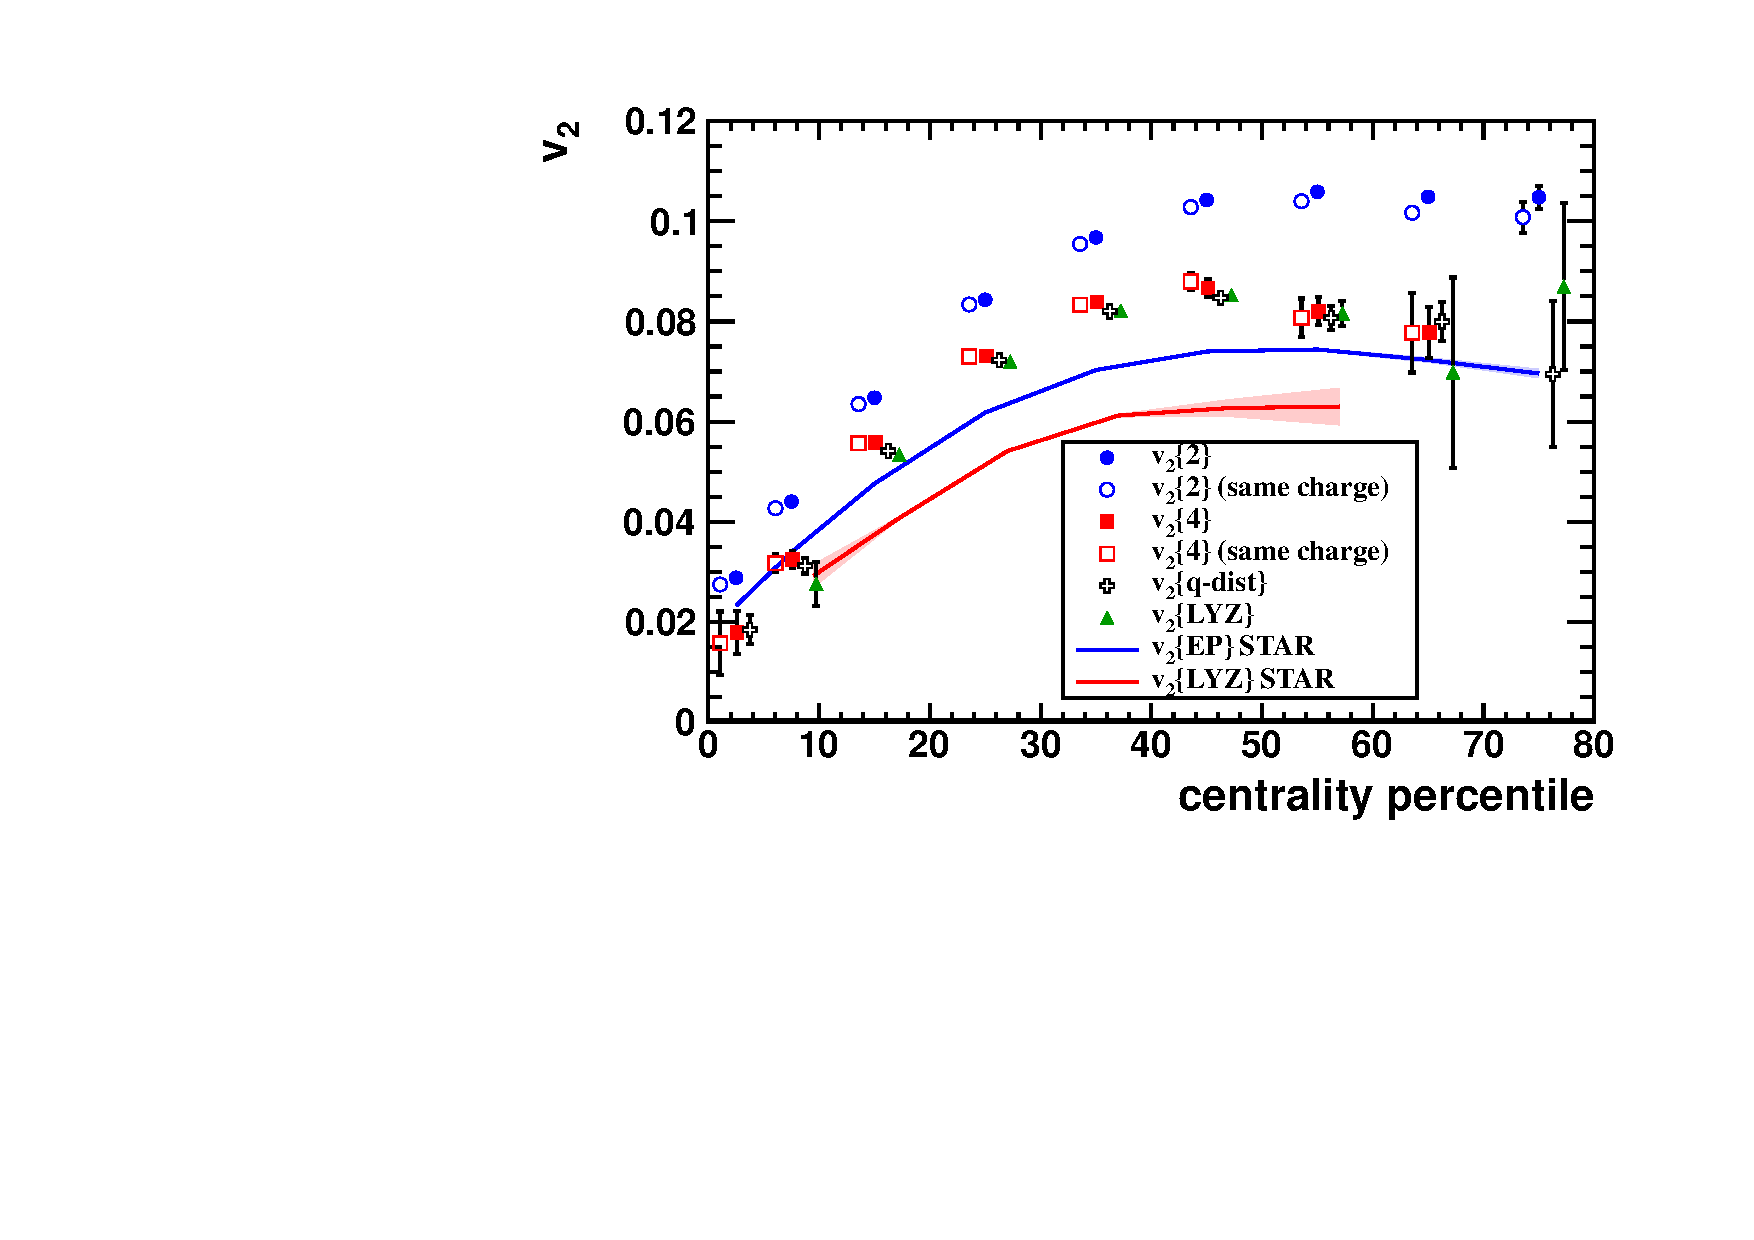
\includegraphics[width=12.0cm]{figures/alice_flow_result}}
\caption{ The published results of flow with ALICE Pb + Pb $\sqrt{S_{NN}}=2.76$~TeV with various methods \cite{Aamodt:2010pa}.} 
\label{fig:alice_flow_result}
\end{figure}


The higher-order cumulants like 6-particle or 8-particle correlation can be calculated in the same way.

\section{Jet quenching}


In $p$-$p$ collisions, hard scattered partons fragment into hadrons with high transverse momentum, also called as jets. However in heavy-ion collisions, the hard scattering occurs before the formation of QGP, and the scattered partons will experience the entire evolution of the system created in these collisions \cite{Enterria:2009am}.
These partons will interact strongly with the created medium and loss their energy, and these features are known as ``jet quenching''  \cite{PhysRevLett.68.1480}. This ``jet quenching" is the another strong evidence of the existence of the QGP, because energy loss in a deconfined matter is believed to be much stronger than in hadronic matter \cite{PhysRevLett.68.1480}. ``Jet quenching" is usually observed with the suppression of high $p_T$ particles yields though the nuclear modification factor $R_{AA}$, defined as like 
 
 \begin{equation}
	R_{AA}(p_{\rm{T}}) = \frac{dN_{ch}^{AA}(p_{\rm{T}})/dp_{\rm{T}}}{\langle N_{coll} \rangle dN_{ch}^{pp}(p_T)/dp_T}
\end{equation}

where AA denotes heavy-ion collisions and $pp$ for the $p$-$p$ collisions. the $dN_{ch}(dp_{\rm{T}})$ refer the number of charged particle produced in each collisions as a function of transverse momentum. The number of binary collisions $N_{coll}$ has been used to compare the yield of charged particle produced in AA and $p$-$p$ collisions as scaling factor. This $N_{coll}$ were calculated by Glauber model, which provide a proper normalization for a given AA centrality. 
  If there are not any medium effects on AA collisions, the heavy-ion collision can be regarded as a just simple superposition of nucleon-nucleon collisions (as like $p$-$p$) and nuclear modification factor $R_{AA}$ will be unity. Otherwise, any deviation from unity of $R_{AA}$  will indicate a certain medium effect of heavy ion collisions. 
  

\begin{figure}[!t]
\centerline{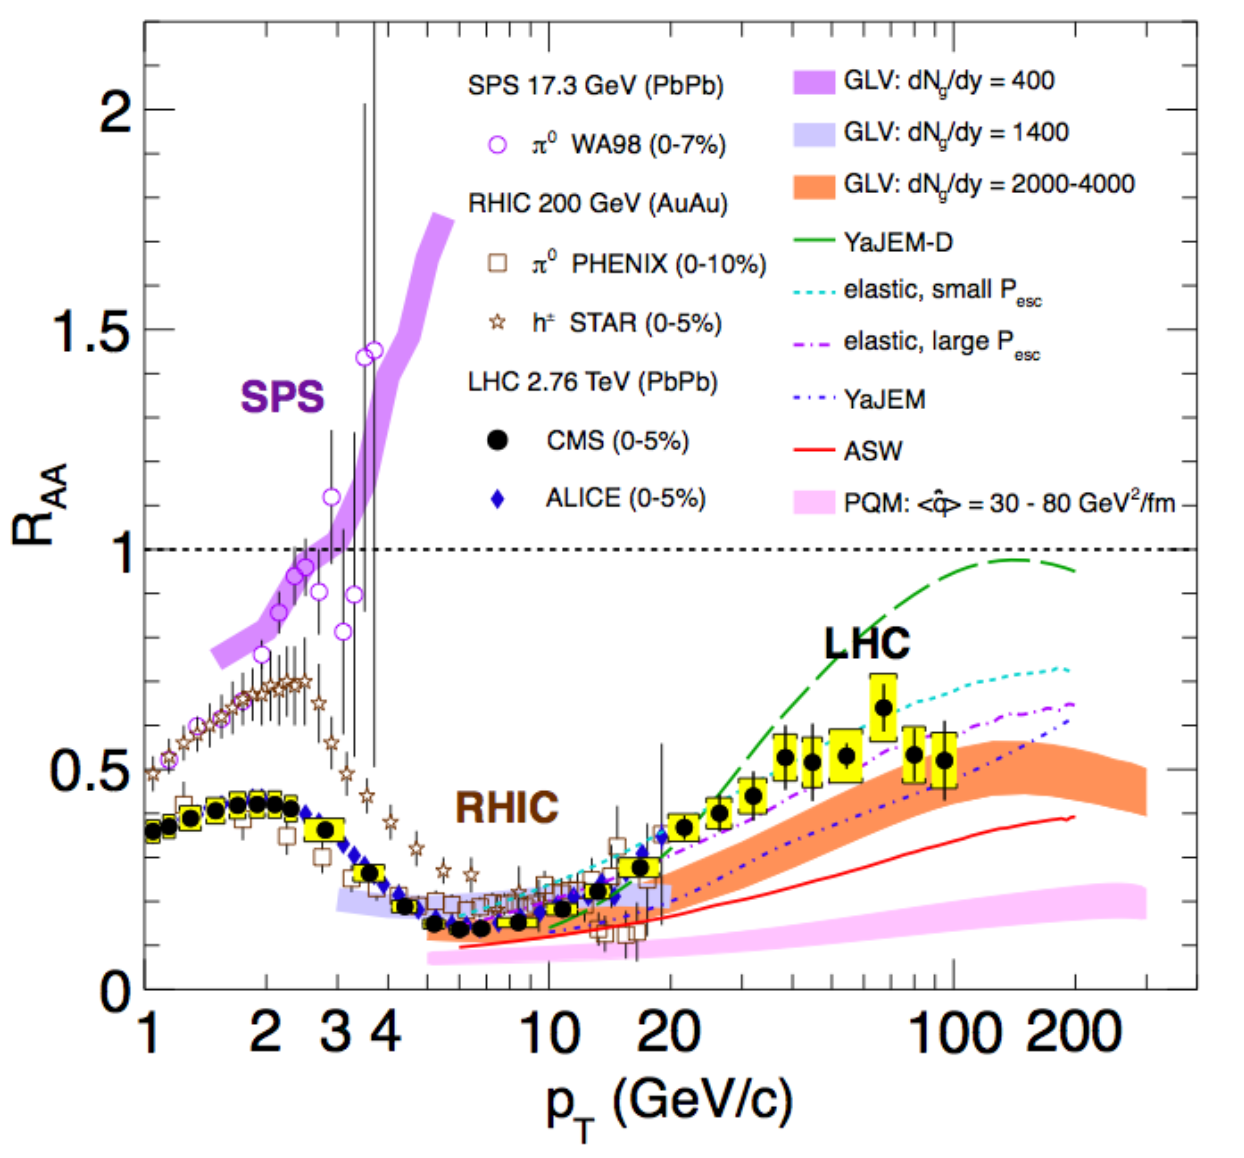
\includegraphics[width=12.0cm]{figures/raa}}
\caption{ Transverse momentum dependence of nuclear modification factor $R_{AA}$ for charged particles produced in heavy ion collisions at SPS, RHIC, and LHC \cite{Roland201470}.} 
\label{fig:RAA}
\end{figure}

    At the energy of SPS, the $R_{AA}$ was slightly lower than unity for $2 < p_T < 3$~GeV/$c$ and almost unity for above $p_T$ \cite{Aggarwaletal.2002}.   However, at RHIC energy, $R_{AA}$ increase monotonically up to $p_T \sim 3$~GeV/$c$ and then start to decrease. Hadron production for $6 < p_T < 8$~GeV/$c$ is suppressed by a factor of 5 in central Au-Au collision when compare to p-p collisions \cite{PhysRevLett.101.232301, PhysRevLett.91.172302}.
    
   Also, at ALICE energy, $R_{AA}$ published in 2010 with the $p_T$ spectra up to 20 GeV/$c$ shows a slightly stronger suppression (about a factor of 7 observed for the $p_T$ range around 6$\sim$8~GeV/$c$) than previous results was reported.  This observation was confirmed by CMS Collaborations, which extended to $p_T$ range up to 100~GeV/$c$. The $R_{AA}$ measurements exhibit a clear increasing trend up to $p_T \sim 40$~GeV/$c$ and then seems to saturate with a value of about 0.5. 
   
   
    In addition, the parton energy loss in created medium is increase as the path-length. The path-length which hard scattered parton travels are related to local geometry of create medium. Since in non-central collision the shape of collision regions are formed as like ellipse, the path-length will depend on the azimuthal angles respect to reaction plane angle. For instance, the parton travels along the minor-axis direction (in plane direction) have shorter path-length than the parton emit to the direction of major-axis (out of plane direction). As the results, at high $p_T$, $v_2$ is expected to be due to ``jet quenching'' reflecting the azimuthal asymmetry of the path-length \cite{Christiansen:2016uaq}.
    
    The study of jet energy loss in created medium as function of path-length are performed by utilizing $R_{AA}(p_{\rm{T}})$ and $v_2(p_{\rm{T}})$.  The path-length as the function of centrality and azimuthal angle respected to 2nd event plane ($\sim$ reaction plane) were estimated from Glauber simulation and details can be found in Appendix C.    
    
    
\clearpage
\section{Correlation between flow harmonics}

 Since the early 1990s the second order flow$(v_2)$ was studied as one of the most interesting results at RHIC, with Au+Au $\sqrt{S_{NN}}=200$ GeV collisions. This large signal of  the second order ``elliptic flow" are explained by the almond shape of the collision overlap region in initial state, and it indicated that a perfect liquid had been made in the early stage of collision. Also detailed studies about flow study report that the fluctuation over event-by-event leads odd number harmonics flow. 
 
 The anisotropic flow is understood as hydrodynamic response to spatial deformation of the initial density profile.
This profile fluctuates event to event due to quantum fluctuations of the positions of the constituents inside the colliding nuclei, which implies that the flow also fluctuates~\cite{Miller:2003kd,Alver:2006wh}.
The recognition of the importance of flow fluctuation has led to triangular flow and higher harmonics~\cite{Alver:2010gr,ALICE:2011ab} as well as the correlations between different Fourier harmonics~\cite{Aad:2014fla}.
 As the result from ATLAS experiments, it shows that higher order harmonics are sensitive to the $\eta/s$~\cite{Luzum:2012wu}.
And the $v_{n}$ distributions carry detailed information about the initial density profile~\cite{Renk:2014jja,Yan:2014nsa}.

However, difficulties on extracting the shear viscosity in heavy ion has been realized since it strongly depends on the specific choice of the initial conditions~\cite{Romatschke:2007mq,Luzum:2012wu,Shen:2011zc}.
The viscous effects reduce the magnitude of the elliptic flow. Furthermore, the magnitude of $\eta/s$ used in these calculations should be considered as an average over the temperature history of the expanding fireball while as it is known that $\eta/s$ of other fluids depends on temperature. 
In addition, part of the elliptic flow also can originate from the hadronic phase~\cite{Bozek:2011ua,Rose:2014fba,Ryu:2015vwa}. Therefore,
knowledge of both the temperature dependence and the relative contributions from the partonic and hadronic phases should be understood better to quantify $\eta/s$ of the partonic fluid.

The higher harmonics ($n>3$) are understood as superpositions of linear and nonlinear responses, through which they are correlated with lower-order harmonics ~\cite{Teaney:2012ke,Bravina:2013ora}. When the harmonic order is large, the nonlinear response contribution in viscous hydrodynamics is dominant~\cite{Teaney:2012ke,Bravina:2013ora}.
The magnitude of the viscous corrections as a function of $p_T$ for $v_4$ and $v_5$ are sensitive to ansatz used for the viscous distribution function, $\delta f$, a small correction for the equilibrium distribution at hadronic freeze-out when QGP phase has become cool and dilute~\cite{Luzum:2010ad}.
Hence the studies of the higher order ($n>3$) to lower order ($v_2$ or $v_3$) harmonic correlations and their $p_T$ dependence can help to understand the viscous correction to the momentum distribution at hadronic freeze-out which is probably the least understood part of hydrodynamic calculations~\cite{Teaney:2012ke,Niemi:2015qia}.


 Although there have been detailed studies of single flow harmonics in recent decades, only a few studies discussed correlation between two different flow harmonics. The difficult part of studying flow correlation is that there are two kinds of correlation between flows: the correlation between two flow magnitudes $(v_n - v_m)$, and the correlation between two flow directions. i.e., event plane angles correlation for two different flow harmonics ($\psi_n - \psi_m$).
 
 ATLAS Collaboration measured the correlation between different order event plane angles with two plane or three correlators by using two (three) subevents symmetric around $\eta = 0$ with a gap in between. With this method, we can expect the same resolution for each subevent groups and it provides its own estimate of the event plane (Fig.\ref{fig:atlas}). As a result they found a positive correlation between event plane angles as a function of centrality.
 
 CMS Collaboration also reported the correlation between different order event plane angles by using event plane methods \cite{Chatrchyan:2013kba}, which measure higher-order flow (like $v4, v5, v6$) with its own event plane angle, and also with the event plane angle which are measured from lower harmonics. For example, Fig.\ref{fig:cmsevtp} compares the $v_4$ with its own event plane angle $\Psi_4$ (i.e. $v_4\{\Psi_4\}$) and $v_4$ with 2nd order flow event plane angle $\Psi_2$ (i.e. $v_4\{ \Psi_2 \}$). 

\begin{figure}[h]
\centerline{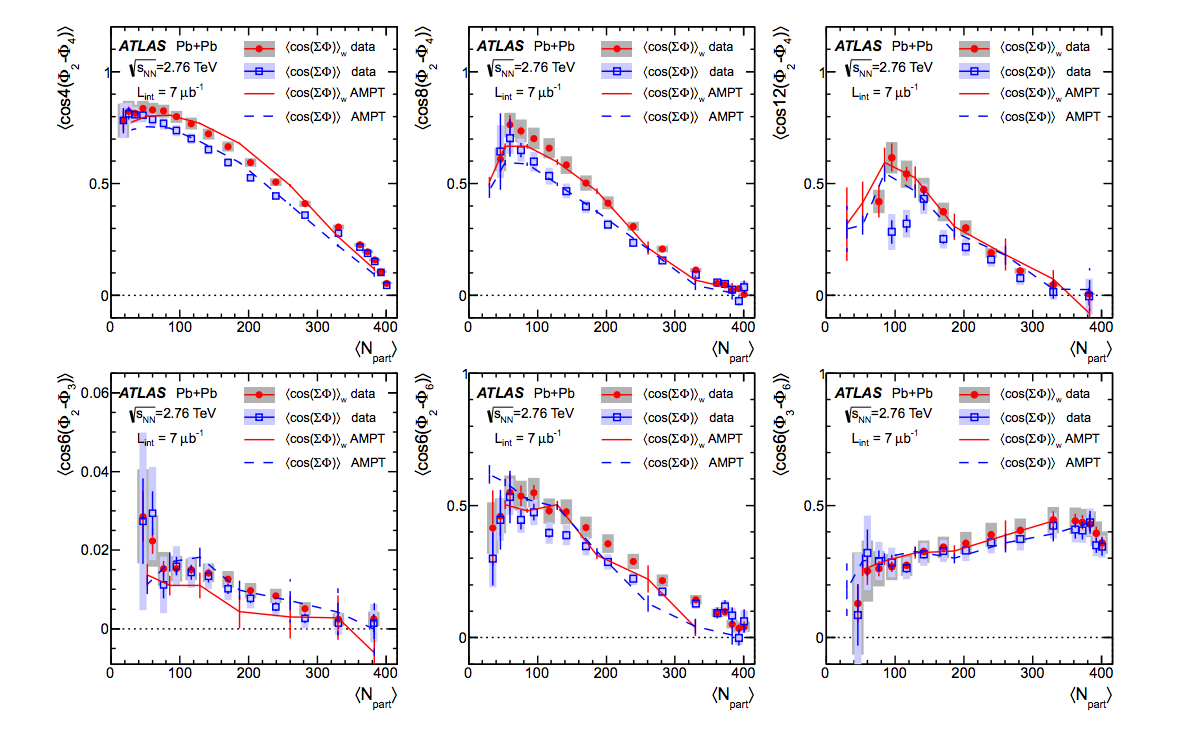
\includegraphics[width=12.0cm]{figures/atlas_eventcorr}}
\caption{ The two event plane correlators by using two subevent groups by ATLAS collaboration. $\langle \sum \Phi \rangle \equiv \langle jk(\Phi_n - \Phi_m) \rangle$.  Results from the AMPT model calculation via the SP method(solid line) and the EP method(dashed line) for represent for comparison \cite{Aad:2014fla}.} 
\label{fig:atlas}
\end{figure}


\begin{figure}[h]
\centerline{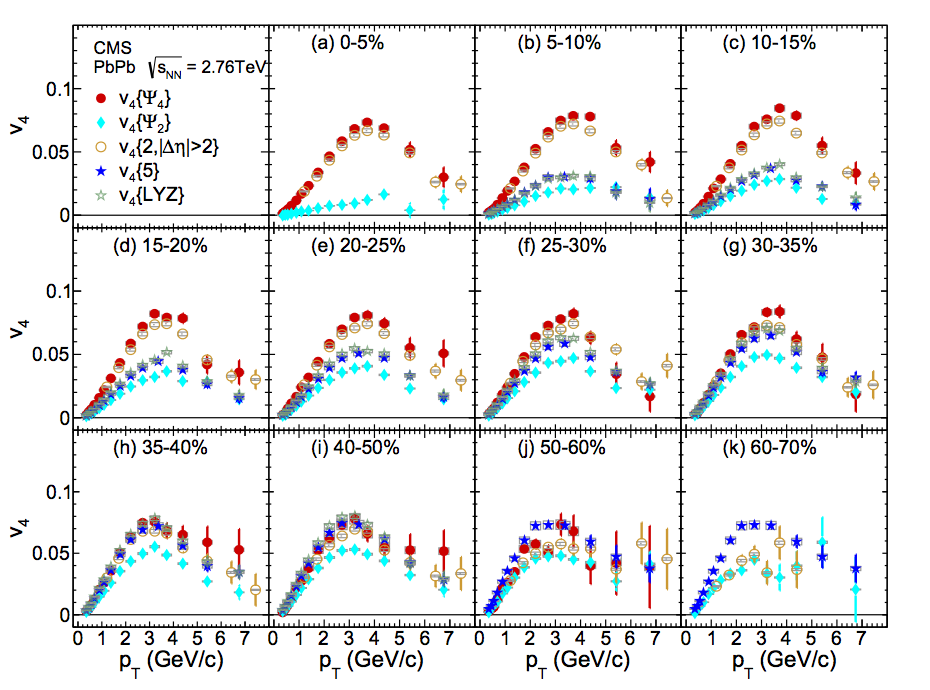
\includegraphics[width=12.0cm]{figures/cms_vn_evt}}
\caption{ Measurement of $v_4$ with different methods as a function of $p_T$ for the indicated centrality bins. The event plane method with its own event plane(red circle) and the event plane method with 2nd order event plane (blue diamonds) are drawn together.\cite{Chatrchyan:2013kba} } 
\label{fig:cmsevtp}
\end{figure}

Despite several approaches in studying flow correlations, it is still a challenge to measure only ``direction" and ``magnitudes" correlations independently. One observable proposed by H. Niemi et al. \cite{PhysRevC.87.054901} can be used to study the event-by-event fluctuations and also can measure the correlations between different $v_n$ which directly related to $\epsilon_n$. They define the linear correlation coefficients $c(a, b)$ as : 

\begin{equation}
	c(a,b) = \left\langle \frac{(a-\langle a \rangle_{ev})(b-\langle b \rangle_{ev})}{\sigma_a \sigma_b} \right \rangle_{ev}
\end{equation}
\smallskip


where $\sigma_a$ is the standard deviation of the quantity $a$. This correlation function is 1 (or -1) if $a$ and $b$ are linearly (anti-linearly) correlated and zero in the absence of correlation. From this calculation with hydrodynamic models, correlation between flow harmonics was found. The result indicates that the correlation not only depends on $\eta/s$, but is also strongly sensitive to the other properties of the QGP, such as decoupling temperature. Otherwise, the correlation $v_2$ and $v_3$ seems sensitive to the initial conditions but insensitive to $\eta/s$. Also clear $p_T$ dependence on correlation $c(v_2, v_3)$ was expected.  

Recently we measured for the first time the new multiparticle observables, the Symmetric 2-harmonic 4-particle Cumulants (SC), which quantify the relationship between event-by-event fluctuations of two different flow harmonics \cite{PhysRevC.89.064904}. The new observables are particularly robust against few-particle non-flow correlations and they provide orthogonal information to recently analysed symmetry plane correlators~\cite{ALICE:2016kpq}. 
It was demonstrated that they are sensitive to the $\eta/s$ of the expending medium and simultaneous descriptions of different order harmonic correlations would constrain 
both the initial conditions and the medium properties.
In this article, we have extended the analysis to higher order Fourier harmonic (up to 5th order) correlations as well as $p_T$ dependence of correlations for the lower order harmonic ($v_3$-$v_2$ and $v_4$-$v_2$).  We also include a systematic comparison to hydrodynamic and AMPT models.
 
   From these studies, we can understand that the flow harmonics fluctuate event-by-event due to the fluctuations in the initial matter distribution, including contributions from fluctuations in the positions of the participating nucleons in the nuclei, the participant plane, determined by the participating nucleons. In addition, such event-by-event fluctuations of the spatial asymmetry generate additional harmonics, which are more sensitive to $\eta /s$, because the effect of share viscosity reduces all anisotropic flow coefficients, with a larger decrease for higher order coefficients.  
 
\clearpage
% !TEX root = main_org.tex


\chapter{Experimental setup}
\section{Large Hardon Collider}

The Large Hadron Collider is the biggest accelerator in the world which wasbuilt between 2002 and 2009 at CERN. This powerful  particle accelerator was installed in the 27km long circular underground tunnel across the border between France and Swiss. It has 16 RF(radio frequency) accelerating cavities and over 1600 superconducting magnets. With this accelerator, we can collide protons with a centre-of mass energy up to 14 TeV and Pb ions with a centre-of mass energy per nucleon up to 5.5 TeV \cite{lhc}.

The protons are first accelerated in linear accelerator LINAC and injected into the BOOSTER at an energy of 50 MeV. The BOOSTER accelerates them to 1.4 GeV before they are sent to the Proton Synchrotron (PS), which further accelerates the protons to 25 GeV.  From the PS they are sent to the Super Proton Syncrotron (SPS), where they yet again are accelerated, this time to 450 GeV. Finally they are transferred to the LHC ring. At Maximum the 2808 bunches of the protons traevel the ring either clockwise or counter- clockwise.

Procedures for operating the LHC with lead ions are similar, though with some differences. The lead ions are produced by heating a highly purified lead sample up to around 550$^\circ$. This creates a number of charge states, with Pb$^{27+}$ being the dominant one. The ions are accelerated in LINAC 3 to 4.2 MeV per nucleon. Afterwards they are sent through a carbon foil, which strips them to Pb$^{54+}$.  The Pb$^{54+}$ beam is leaded to the Low Energy Ion Ring (LEIR), where it is accelerated to 72 meV per nucleon, before being transferred to the PS. At the PS, the ions are accelerated up to 5.9 GeV per nucleon. The ions once again are sent through the foil, stripping them to Pb$^{82+}$, which is the final ionization used for collisions. After the PS the now fully stripped ions arrive at the SPS, where they are accelerated to 177 GeV per nucleon, before being sent into the LHC ring for acceleration to their collision energy($0.999999991c$ at $\sqrt{s_{NN}}=7$TeV). As in the proton case, the ion bunches are sent either clockwise or counter-clockwise around the ring. The collision of lead ions only occur at 3 of the experiment sites, namely ALICE \cite{alice}, ATLAS \cite{atlas}, and CMS \cite{cms}. The ATLAS and CMS experiments are general purpose detectors used to look for signs of new physics, including the origins of the mass of elementary particles and extra dimensions. The ALICE detector is designed to study the properties of the so called quark gluon plasma (QGP) which is believed to have been created in the first microseconds after the Big Bang. Details will be discussed in the following chapter.


     \begin{figure}[!h]
		\begin{center}
        	\resizebox{0.85\columnwidth}{!}{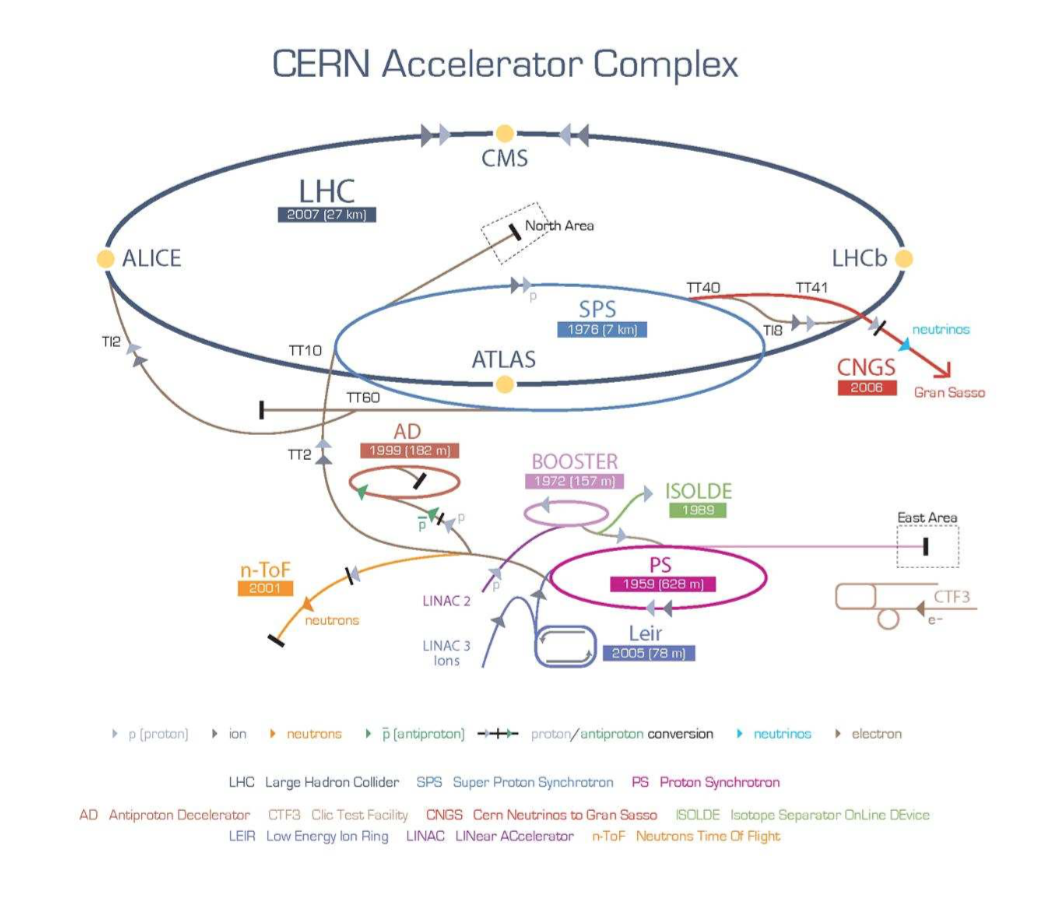
\includegraphics{figures/lhc}}
        	\caption{Schematic view of Large Hadron Collider}
        	\label{lhc}
        \end{center}
    \end{figure}


\section{The ALICE experiment}

ALICE (A Large Ion Collider Experiment) is one of the experiments placed in LHC. The collaboration involves more than a thousand scientists and engineers from 116 institutes and 33 countries. It was designed to study the properties of QCD and to characterize the Quark-Gluon Plasma (QGP). It is the only experiment at LHC which was optimized for the heavy ions collisions.


     \begin{figure}[!h]
		\begin{center}
        	\resizebox{0.85\columnwidth}{!}{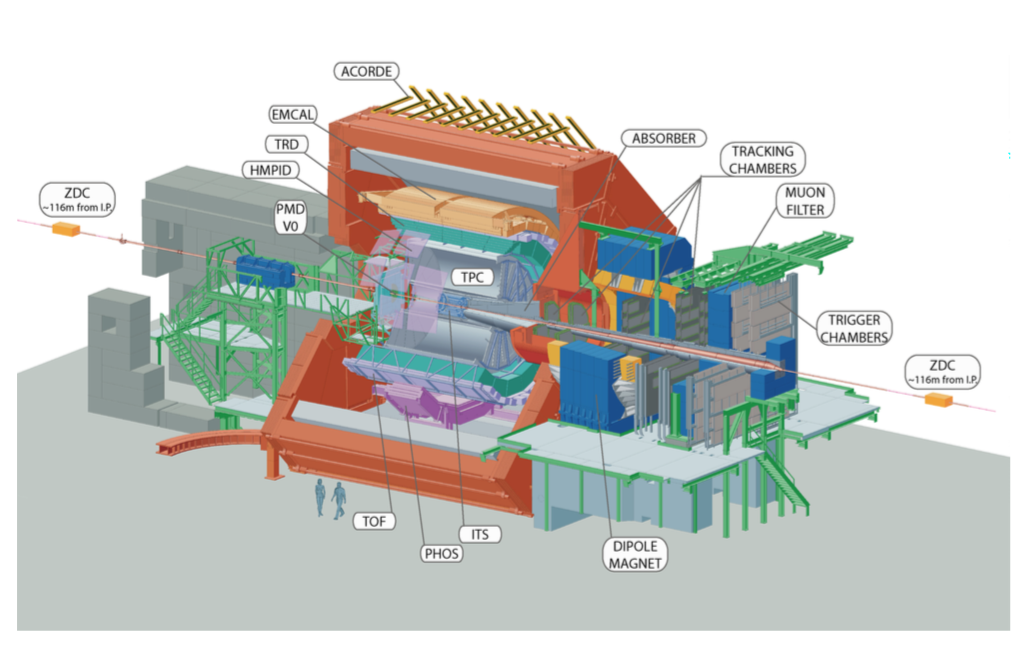
\includegraphics{figures/alice}}
        	\caption{Schematic view of ALICE detector \cite{cds}}
        	\label{alice}
        \end{center}
    \end{figure}

The detector is placed in the solenoid magnet from the L3 experiment. This provides a relatively low magnetic field of 0.5 T, which allows to measure low momentum particles corresponding to the so-called soft QCD, as well a s more energetic particles from hard processes. Because of the extremely high multiplicity expected in nucleus-nucleus collisions at LHC energies, the design of ALICE was optimized for a multiplicity $dN_{ch}/dy = 8000$. ALICE has an efficient and robust tracking system over a large momentum range, from tens of MeV/$c$ (soft physics) to over 100 GeV/$c$ (jet physics). As some of the tracking detectors are based on drift technologies, they are slower then the detectors operated by the other LHC experiments but can work at the nominal LHC ion beam rate of 10 kHz. A specificity of the ALICE detector over the other LHC experiments is its emphasis on hadron and lepton identification (PID). It is achieved over much of the momentum range using most known PID techniques, such as $dE/dx$ energy loss, time-of-flight, transition and Cherenkov radiation, electromagnetic calorimetry, muon filters, and topological decay reconstruction.

The detectors in the ALICE experiment are arranged in a classical layered structure around the interaction point as Shown in Figure.\ref{alice}. Here is a short description of the main detectors which used in this analysis. Most of description here are taken from the ALICE Technical Design Report (ALICE TDR) \cite{Cortese:879894}, and more detail information can be found in CERN document system (CDS) \cite{cds}.



\subsection{ITS}

The Inner Tracking System (ITS) consists of six layers of silicon detectors with radii few cm as shown Figure.\ref{its}

     \begin{figure}[!h]
		\begin{center}
        	\resizebox{0.85\columnwidth}{!}{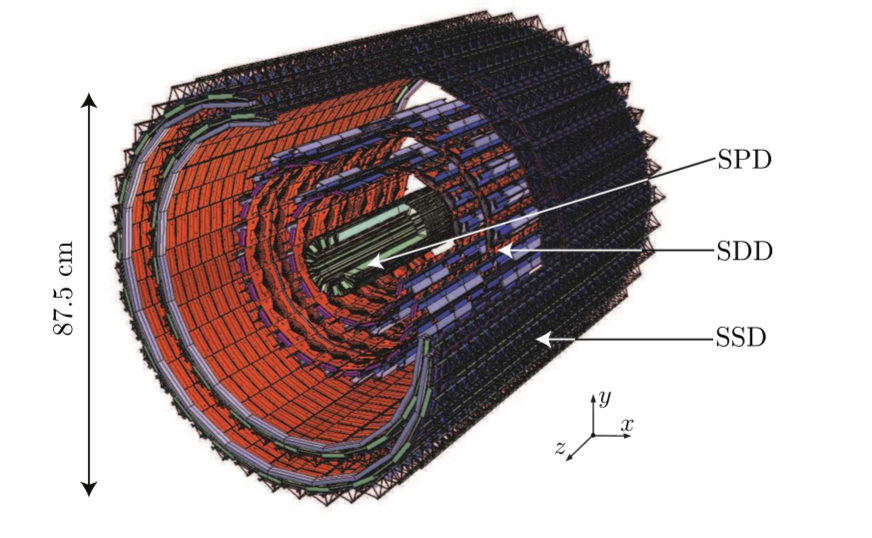
\includegraphics{figures/its}}
        	\caption{ALICE Inner Tracking System(ITS), includes Silicon Pixel Detector(SPD) and Silicon Drift Detector(SDD) and Silicon Strip Detector(SSD)}
        	\label{fig:its}
        \end{center}
    \end{figure}


The main purpose of the ITS is the reconstruction of the primary vertex of the collision as well as the reconstruction of secondary vertexes with a resolution better than 100 $\mu$m in transverse direction. The ITS stand-alone tracking can provide the tracking information for low-momentum particles that do not reach the TPC. The $p_T$ cut-off at nominal field for the two innermost layers is about 35 MeV/c.

The two innermost layers, Silicon Pixel Detector (SPD) \cite{Meddi200140}, are based on hybrid silicon pixels which consist of silicon detector diodes with a thickness of 200 $\mu$m. The first layer and the second layer are placed at 3.9 cm and 7.6 cm with an acceptance of $|\eta| < 2.0$ and $|\eta| < 1.4$, respectively. The SPD has approximately 10 million channels. The pixel readout chip (ALICE1LHCb) is a mixed- signal ASIC for the readout of 8192 pixels. Each pixel cell contains a preamplifier-shaper with leakage current compensation, followed by a discriminator. A signal above threshold results in a logical 1 which is propagated through a delay line during the 6 $\mu$s latency time until the arrival of the L1 trigger signal. Upon arrival of the L1 trigger, the logical level present at the end of the delay line is stored in the first available buffer location. The outputs of the discriminators in the pixel cells of the ALICE1LHCb chip provide a fast-OR digital pulse when one or more pixels are hit on the chip. 

The third and forth layer, Silicon Drift Detector (SDD) \cite{Alessandro:2010rq}, consist of a 300 $\mu$m thick layer of homogeneous high-resistivity silicon. The readout of the SDD is analog, therefore particle identification can be conducted using the information of energy-loss. The SDD has 133,000 channels.

The two outermost layers, Silicon Strip Detector (SSD) \cite{Contin:2011rs}, consist of sensors equipped on both sides with silicon micro-strips. These are arranged under a stereo angle of 35 mrad allowing for a two-dimensional measurement of the track position together with an energy-loss measurement for particle identification. The SSD has approximately 2.6 million channels \cite{Contin:2009lza}.



\subsection{TPC}

The Time Projection Chamber (TPC) \cite{CERN-LHCC-2013-020} is the main tracking device of the ALICE experiment. It is a large cylinderical gas chamber detector with $\sim 88$m$^3$ volume in 0.5 T solenoidal magnetic filed parallel to the E field. 

This detector is designed to have $dE/dx$ resolution better than 5\% and a relative $p_T$ resolution better than 1\% for momenta of $\sim 1$GeV/$c$ and better than 2.5\% for momenta of 4GeV/$c$, and two track resolution capable of separating tracks with a relative momentum difference of $< 5$MeV.

The TPC is separated by two volumes with the Central Electrode (CE) made of single stretched Mylar foil, and secondary electrons drift toward the end-caps. 

\begin{figure}[!p]
\centerline{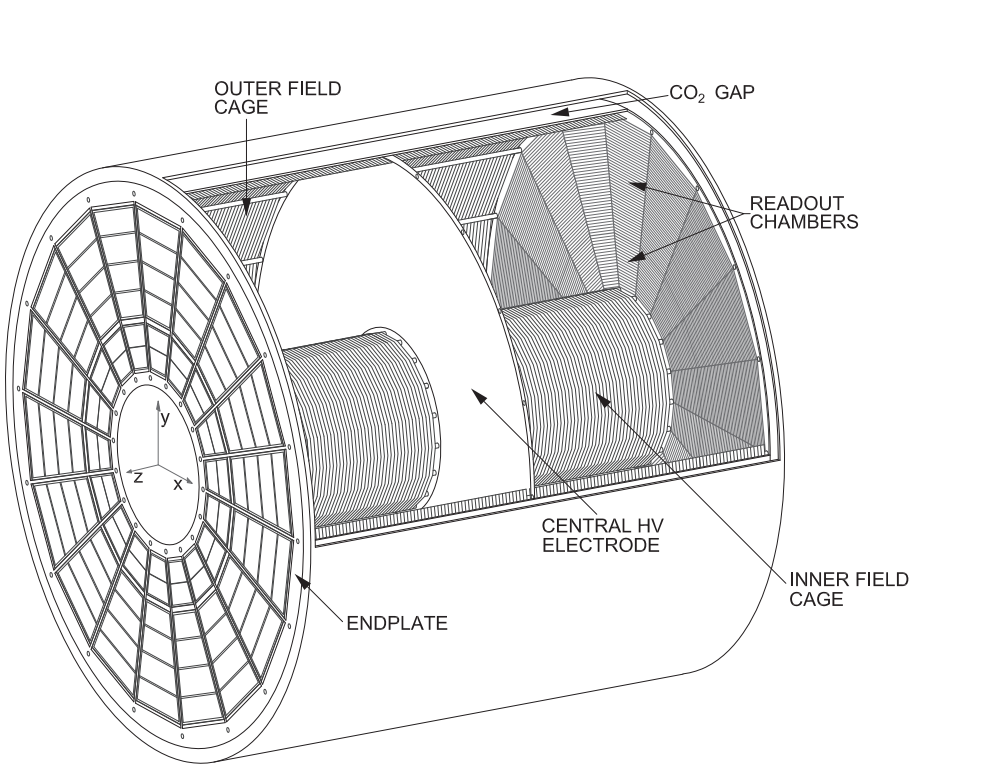
\includegraphics[width=10.0cm]{figures/tpc1}}
\centerline{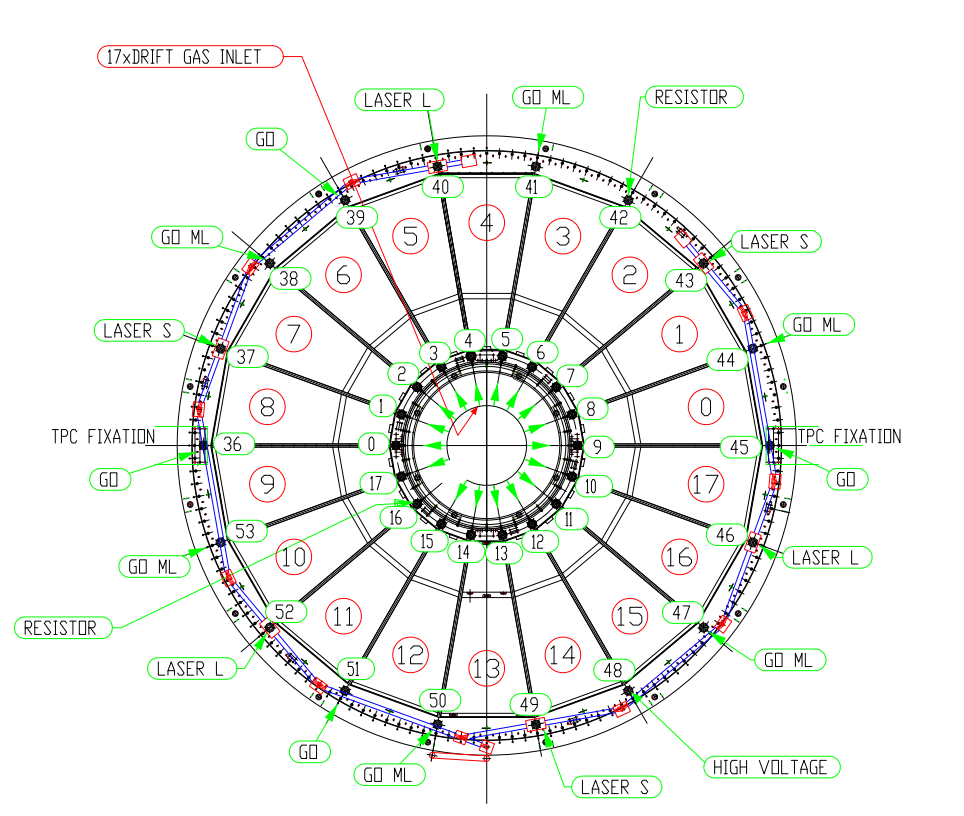
\includegraphics[width=10.0cm]{figures/tpc2}}
\caption{ ALICE Time Projection Chamber } 
\label{fig:cmsevt}
\end{figure}


Volumes are filed with Ne-CO$_2$-N$_2$ (90\%-10\%-5\%) gas which is optimized for drift speed, ion mobility, and low diffusion of electrons. Since, Ne-CO$_2$-N$_2$ gas have dependence of drift velocity on temperature, TPC is aiming for a thermal stability with $\Delta T < 0.1$K in the drift volume over the running period. 

As the gas detector, the TPC field cage has to be operated at very high voltage gradients, of about 400V/cm, with a high voltage of 100kV at the central electrode which results in a maximum drift time of about 90$\mu$s.

The TPC covers a pseudo-rapidity range of $|\eta| < 0.9$ for full track length within the TPC volume. Also it provides 0 to $2\pi$ azimuthal coverage except for the dead zones in the TPC, and it makes the TPC an ideal detector for anisotropic flow analysis, since these inefficiencies in the  azimuthal acceptance would result in non-negligible systematic biases for the azimuthal angle correlations analysis.



\subsection{VZERO}

The VZERO detectors(also often called V0) \cite{collaboration2013performance} are designed with a much larger acceptance, in order to perform as a minimum bias trigger in both proton-proton and Pb–Pb collisions. Furthermore, it is also used, together with the timing information of the collision, for the rejection of beam-gas interactions. The VZERO is also used to determine the event centrality and many of ALICE analyses use centrality determination from VZERO.

\begin{figure}[!h]
		\begin{center}
        	\resizebox{0.85\columnwidth}{!}{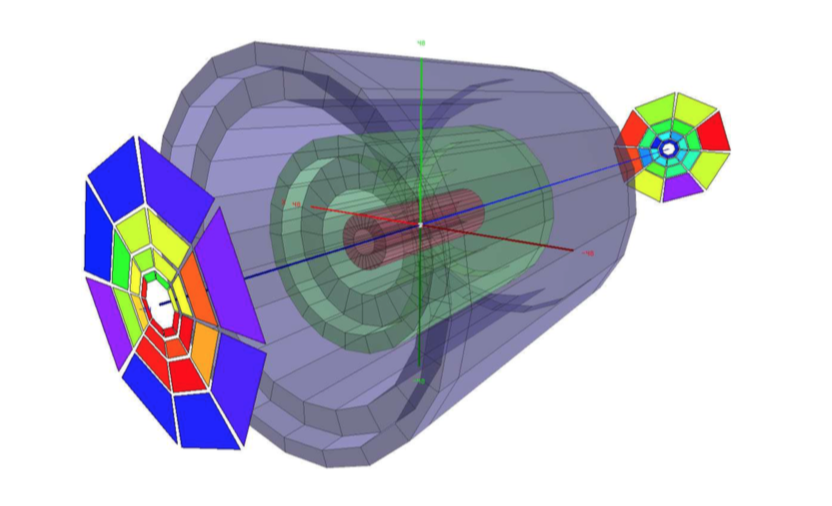
\includegraphics{figures/v0}}
        	\caption{ALICE VZERO detectors on both side of TPC}
        	\label{its}
        \end{center}
    \end{figure}


This consists of two separate arrays of scintillator counters and V0A and V0C, placed on different sides of the central barrel detectors along the beam line. V0A/C are placed asymmetrically with respect to the interaction point. V0A is located 340 cm from the interaction point on the side opposite to the muon arm, while V0C is placed 90 cm from the interaction point on the opposite side from V0A. Because of this asymmetry, V0A and V0C have different pseudo-rapidity coverage. The V0A covers pseudo-rapidity range $2.8 < \eta < 5.1$, while V0C covers $-3.7 < \eta < -1.7$.

The V0A/V0C are segmented into 32 elementary counters distributed in four rings. Each ring covers 0.4-0.6 unit of pseudo-rapidity. The rings are divided into eight sectors of 45$^{\circ}$. The elementary counter consists of scintillator material with embedded WaveLength Shifting (WLS) fibers. The light from the WLS is collected by clear fibers and transported to PhotoMultiplier (PM) installed at 3-5 m from the detectors, inside the L3 magnet. The time resolution of each individual counter will be better than 1 ns.

Signals from each PMT are sent to an electronics circuit, which delivers two signals. The first one is sent to a threshold discriminator for the generation of the V0 event triggers. It is amplified by a factor of about 10. If at least one discriminator is fired during the time window around the timing of the beam crossing (after 3 ns for V0A, 11 ns for V0C), the V0 event trigger is issued.

\subsection{Other detectors}

\subsubsection{TRD}
Transition Radiation Detector (TRD) \cite{Cortese:519145} is placed from 2.9 to 3.8 m from the interaction point. It discriminates electrons from pions with high efficiency for momenta about 1 GeV/$c$ by the identification of the transition radiation photons from electrons. Also this detector can provide the trigger signals for electron 

\subsubsection{TOF}
Time Of Flight (TOF) \cite{alici2013mrpc} is made of Multigap Resistive Plate Chamber strips (MRPC), which are made by a ten layer double-stack detector with a time resolution of about 40 ps. By measuring the time particles take to reach it, and combined with the tracking information of the TPC, it allows for the identification of pions, kaons and protons

\subsubsection{HMPID}
High Momentum Particle Identification Detector (HMPID) \cite{Molnar:2008pr} consists of an array of proximity-focusing Ring Imaging CHerenkov counters (RICH) and covers a pseudo-rapidity range of $|\eta| < 0.6$ and 58$^{\circ}$ of azimuthal angle. The HMPID discriminates pions and kaons in the range $1<p_T<3$GeV/$c$ and protons and kaons in the range $2<p_T<5$GeV/$c$ by means of their Cherenkov rings.

\subsubsection{PHOS}
PHOton Spectrometer (PHOS) \cite{1742-6596-160-1-012045}  is placed partially opposite to the EMCAL and made of highly segmented electromagnetic calorimeter of lead-tungstenate (PbWO4 , PbWO) crystals with a radiation length of 20X$_0$. It is used for neutral mesons and direct photon measurements.

\subsubsection{EMCAL}
ElectroMagnetic Calorimeter (EMCAL) \cite{rene2010alice} is a lead scintillator sampling calorimeter that covers an azimuthal angle range of 107$^{\circ}$ in the rapidity interval $|\eta|<0.7$ at a radial distance of about 4.5 m from the vacuum tube. The EMCAL is designed for the study of jet-physics and can provide trigger signals for hard jets, photons and electrons.

\subsubsection{Muon Spectrometer}

Muon Sepctrometer is situated in the forward($-4 < \eta < -2.5)$) region on one side of the experiment. It track muons with momentum $p > 4$GeV/$c$. And used for the analaysis of quarkonia decaying to the $\mu\mu$.

\subsubsection{TZERO}

TZERO (T0) \cite{cortese2004alice} detector is designed to determine the collision time. T0 consists of two units, one on each side of the interaction point. Each T0 unit is comprised of quartz Cherenkov radiators glued to photo multiplier tubes. A coincidence between signals in both sides is used for both vertex and time determination


\subsubsection{Zero Degree Calorimeter}

The Zero Degree Calorimeters (ZDC) \cite{oppedisano2009physics} are positioned at extremely forward angles. Their role is to measure the spectator nucleons from heavy ion collisions, in order to estimate the number of participants, and hence the centrality. Furthermore they are also used to determine the event plane. 

\subsection{Analysis Framework}

 The ROOT system is an object-oriented framework (written in C++) developed at CERN in the 90’s and used by various collaborations worldwide as a starting framework on top of which the specific framework needed for particular collaboration is being built. It provides a full set of features needed for event generation, detector simulation, event reconstruction, data acquisition and data analysis. All features are encoded in a set of about 650 classes grouped in about 40 libraries. A vast majority of ROOT classes inherit from the common base class called TObject, which provides default behavior and protocol (e.g. protocol for the object I/O, error handling, sorting, inspection, printing, drawing, etc.) for all objects in the ROOT system, but the standalone classes which can be used as built-in types are also implemented. 

The AliRoot is the specific version of framework which built on the ROOT system. It's optimized for ALICE simulation, alignment, calibration, reconstruction, visualization, quality assurance, and analysis. Most of codes are written in C++ and some parts are written in Fortran.


\begin{figure}[t]
\centerline{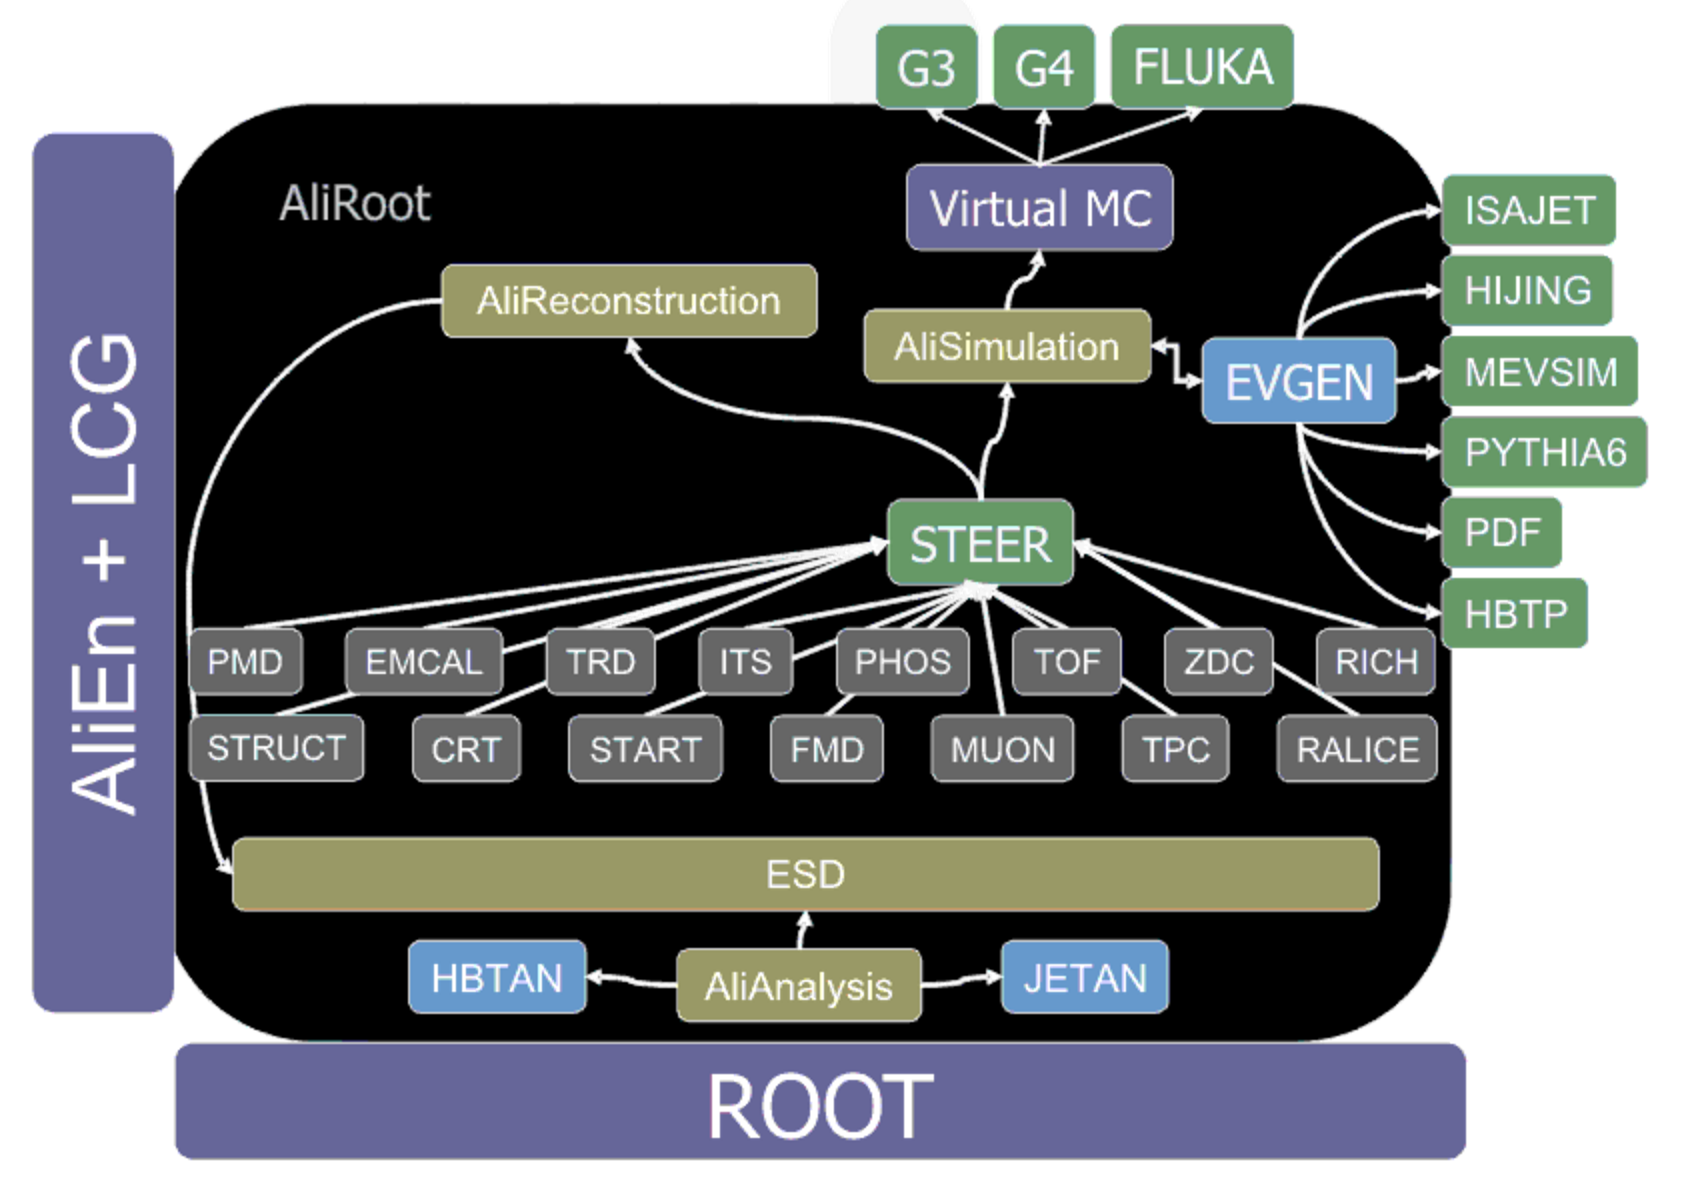
\includegraphics[width=12.0cm]{figures/aliroot}}
\caption{Picture of general schema of the AliRoot architecture \cite{aliroot}} 
\label{fig:cmsevt}
\end{figure}



Also for the large consumption of CPU power, the ALICE analysis framework provides several distributed computing systems, including the parallel computing (PROOF) or, Grid.  Because of the huge amount of data produced by the ALICE detector ($\sim$ 2PB per year) \cite{1742-6596-219-7-072023}, the reconstructed events are saved into a worldwide computing center. The computing center has a distributed hierarchy with Tier 0 to Tier 3, and the ALICE Virtual Organization (ALICE VO) is made of more than 80 sites. Each site provides large computing power with physical machines where the software programs can be run. By using JDL(Job Description Language) and XML(eXecutable Machine Language), users can use codes with AliRoot over 1500 CPUs at the same time.
\clearpage
% !TEX encoding = UTF-8 Unicode
% !TEX root = main_org.tex
\chapter{Data analysis}
\section{Data selection}

In this chapter, we outline the selection criteria applied for this analysis. Basically, we used LHC10 data with pass 2 reconstruction which marked as ``good run". The period of data taking is LHC10h and it is only data sets from heavy ion collisions from 2010. 



\subsection{Default cuts and settings}
 
 The data sample recorded by ALICE during the 2010 heavy-ion run at the
LHC is used for this analysis. Detailed procedure of the ALICE
data taking can be found
in~\cite{Aamodt:2008zz,Carminati:2004fp,Alessandro:2006yt}. The Time
Projection Chamber (TPC) was used to reconstruct charged particle
tracks and measure their momenta with full azimuthal coverage in the
pseudo-rapidity range $|\eta|<0.8$. Two scintillator
arrays (V0) which cover the pseudo-rapidity ranges $-3.7<\eta<-1.7$
and $2.8<\eta<5.1$ were used for triggering, and the determination of
centrality~\cite{Aamodt:2010cz}. The trigger
conditions and the event selection criteria are identical to those
described in~\cite{Aamodt:2010pa, Aamodt:2010cz}.
Approximately $10^7$ minimum-bias Pb-Pb events with
a reconstructed primary vertex within $\pm 10$ cm from the nominal
interaction point in the beam direction are used for this
analysis. Charged particles reconstructed in the TPC in $|\eta|<0.8$
and $0.2<p_T<5$ GeV/$c$ were selected. The charged track quality cuts
described in~\cite{Aamodt:2010pa} were applied to minimize
contamination from secondary charged particles and fake tracks. The
charged particle track reconstruction efficiency and contamination
were estimated from {\sc HIJING} Monte Carlo
simulations~\cite{Wang:1991hta} combined with a {\sc
GEANT3}~\cite{Brun:1994aa} detector model, and found to be independent of
the collision centrality. The reconstruction efficiency increases from
70\% to 80\% for particles with $0.2<p_T<1$~GeV/$c$ and remains
constant at $80 \pm 5$\% for $p_T>1$~GeV/$c$. The estimated
contamination by secondary charged particles from weak decays and
photon conversions is less than 6\% at $p_T=0.2$~GeV/$c$ and falls
below 1\% for $p_T>1$~GeV/$c$.
With this choice of low $p_T$ cut-off ($p_T > 0.2$ GeV/$c$) we are reducing event-by-event biases from smaller reconstruction efficiency 
at lower $p_T$, while the high $p_T$ cut-off ($p_T < 5.0$ GeV/$c$) was introduced to reduce the contribution to the anisotropies from jet particles. 


The default estimator for centrality determination in ALICE is obtained from the measurement multiplicity in the VZERO detectors. 

\begin{center} \tiny{
\begin{tabular}{ |c|c c c c c c c c| } 
 \hline
Centrality(\%)&0-5      &5-10     &10-20    &20-30    &30-40     &40-50      &50-60      &60-70\\ 
\hline
b(fm) AMPT    &0.00-3.72&3.72-5.23&5.23-7.31&7.31-8.88&8.88-10.20&10.20-11.38&11.38-12.47&12.47-13.50\\ 
b(fm) HIJING  &0.00-3.60&3.60-5.09&5.09-7.20&7.20-8.83&8.83-10.20&10.20-11.40&11.40-12.49&12.49-13.49\\ 
b(fm) ALICE   &0.00-3.50&3.50-4.94&4.94-6.98&6.98-    &    -9.88 &9.81-      &     -12.09&12.09-\\
 \hline
\end{tabular}
\url{https://twiki.cern.ch/twiki/bin/viewauth/ALICE/CentStudies}
\label{table:impact} }
\end{center}



Also, even though the Inner tracking System (ITS) and the Time Projection Chanmber (TPC) were used as the main tracking devices for ALICE experiment, ITS does not have uniform acceptance. On the other hand, corrections for TPC are negligible due to its uniform acceptance. Because of this, we are going to use TPC only cuts in this analysis, in which the tracks are required to have at least 70 reconstructed space point out of the maximum 159 in the TPC and a $\langle \chi^2 \rangle$ per TPC cluster $\le 4$ (with 2 degrees of freedom per cluster)

Only tracks with a transverse distance of closest approach (DCA) to the primary vertex less than 3 mm
, both in longitudinal and transverse direction, are accepted to reduce the contamination from secondary tracks (for instance the charged particles produced 
in the detector material, particles from weak decays, etc.). 
Tracks with kinks (the tracks that appear to change direction due to multiple scattering, $K^{\pm}$ decays) were rejected.
 

\vskip20mm
\subsection{Data QA}

\subsubsection{ $\eta$ distribution QA} 

 In principle, the multiplicity in each $\eta$ region should be similar (i.e. $N_{Aside} \sim N_{Cside}$). To confirm this similarity of multiplicity in each $\eta$ set, we check $\eta$ distribution for each centrality bins. Also the multiplicity in $\eta < 0$ region  and $\eta > 0$ is compared as ratio. The ratio between number of multiplicity in $\eta>0 $ subgroup and $\eta<0$ subgroups,
was fitted with 0th order polynomial function with unity parameter(i.e $y=1$) run by run. After fitting, $\chi^2 / NDF$ was calculated to check for the same multiplicity in both subset groups for each run, each centralities.  Fig.\ref{dNdetaQA} are the $\eta$ distribution for run number 137135 and the $\chi^2/NDF$ test results over all run. The Run number corresponding Run ID information can be found in Appendix \ref{DataInfo}


	\begin{figure}[!hp]
		\begin{center}
        	\resizebox{0.45\columnwidth}{!}{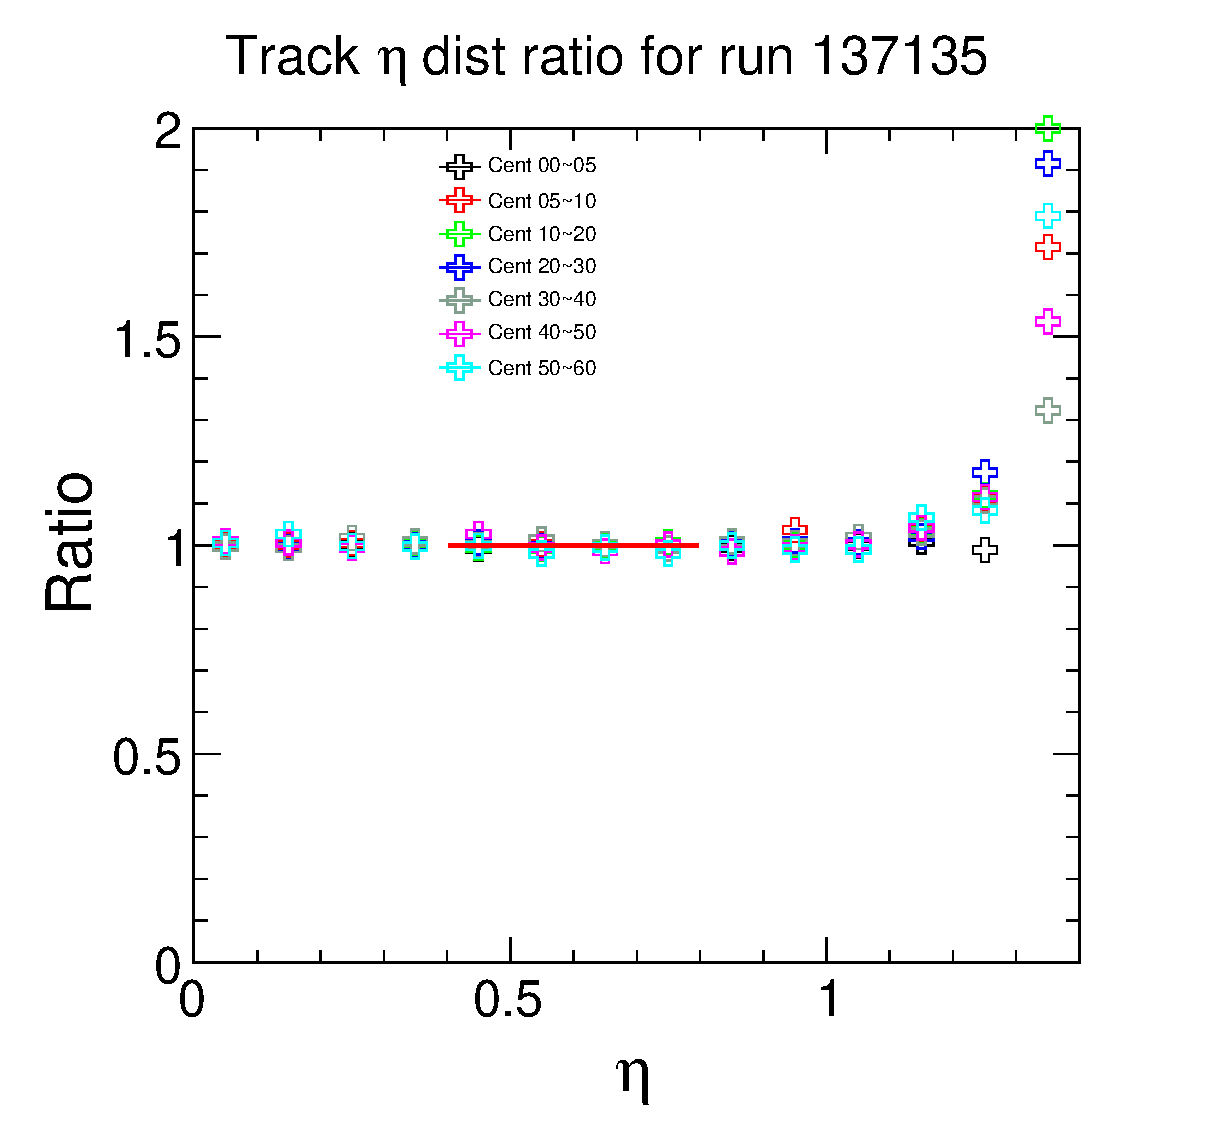
\includegraphics{figures/figs_QA/eta_ratio_run137135_eta_04_08.eps}}
	\resizebox{0.45\columnwidth}{!}{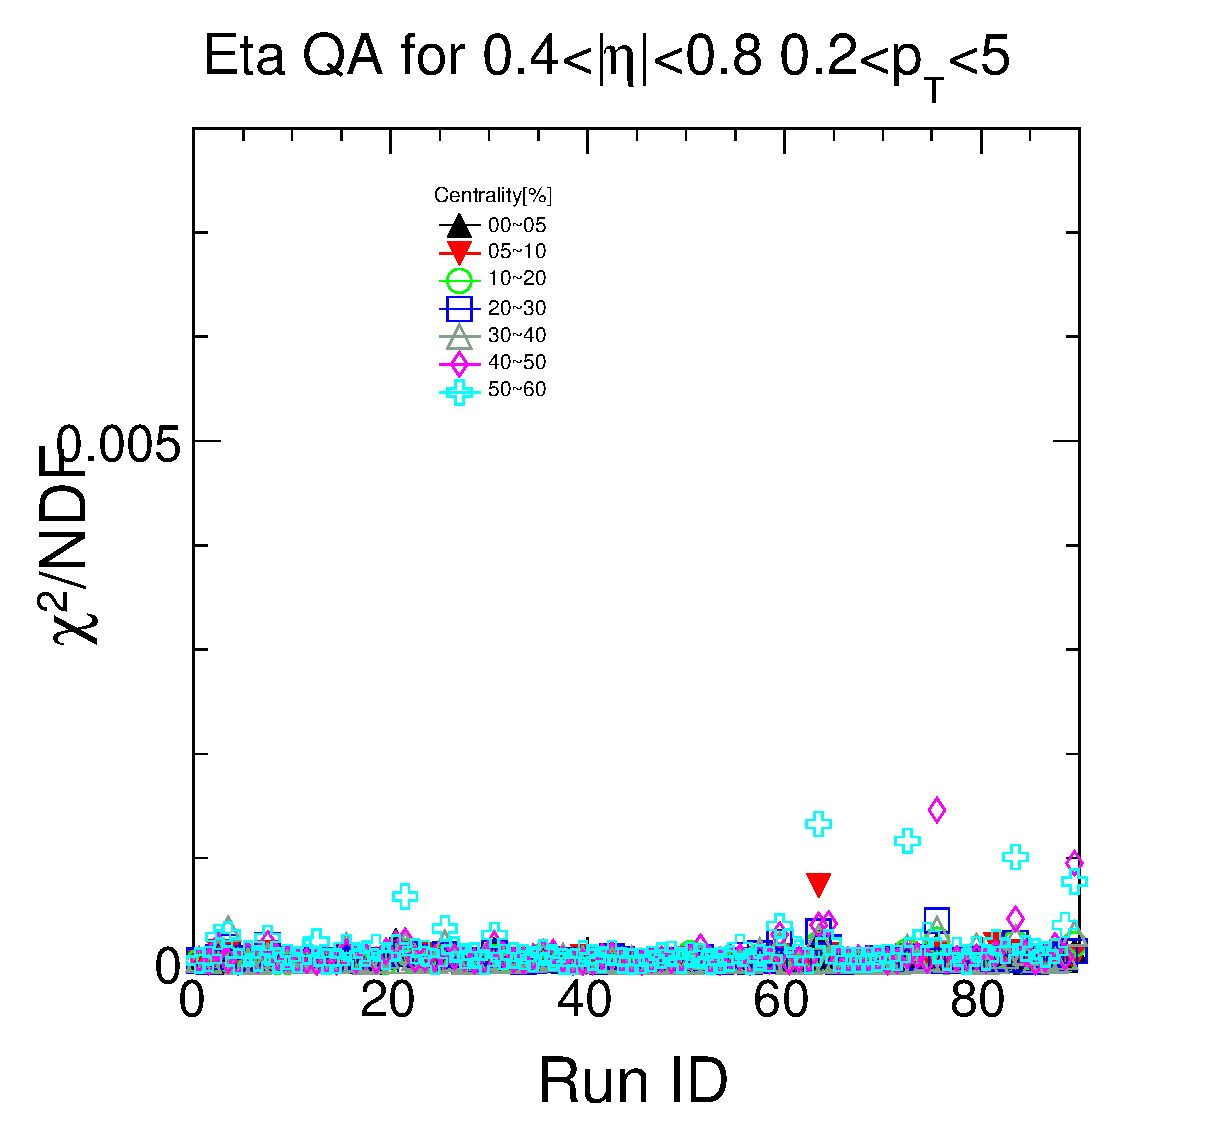
\includegraphics{figures/figs_QA/QA_Eta_ratio_flatness_LHC10h_AOD86.eps}}

        	\caption{Ratio of $dN/d\eta$ for flip over +/- $\eta$ region(left) and $\chi^2/NDF$ for $\phi$ flatness as function of RunID}
        	\label{dNdetaQA}
        \end{center}
    \end{figure}

QA result looks quite good across the runs as shown in figure. $\chi^2/NDF$ was lower than 0.002 for all runs and all centralities. As the results, we might simply assume that number of multiplicity in each subgroups are same.



\subsubsection{ $\phi$ distribution QA}

 $\phi$ flatness QA was performed on the $\phi$ distributions with the data. We fit the distributions with 0th-order polynomial. The distribution was fitted run by run. $\chi^2/NDF$ of each run were taken to estimate the flatness of distribution as like $\eta$ QA method. The fit results are shown in Fig.\ref{fig:QC_phi_chi2NDF}
 
    \begin{figure}[hp]
		\begin{center}
        	\resizebox{0.45\columnwidth}{!}{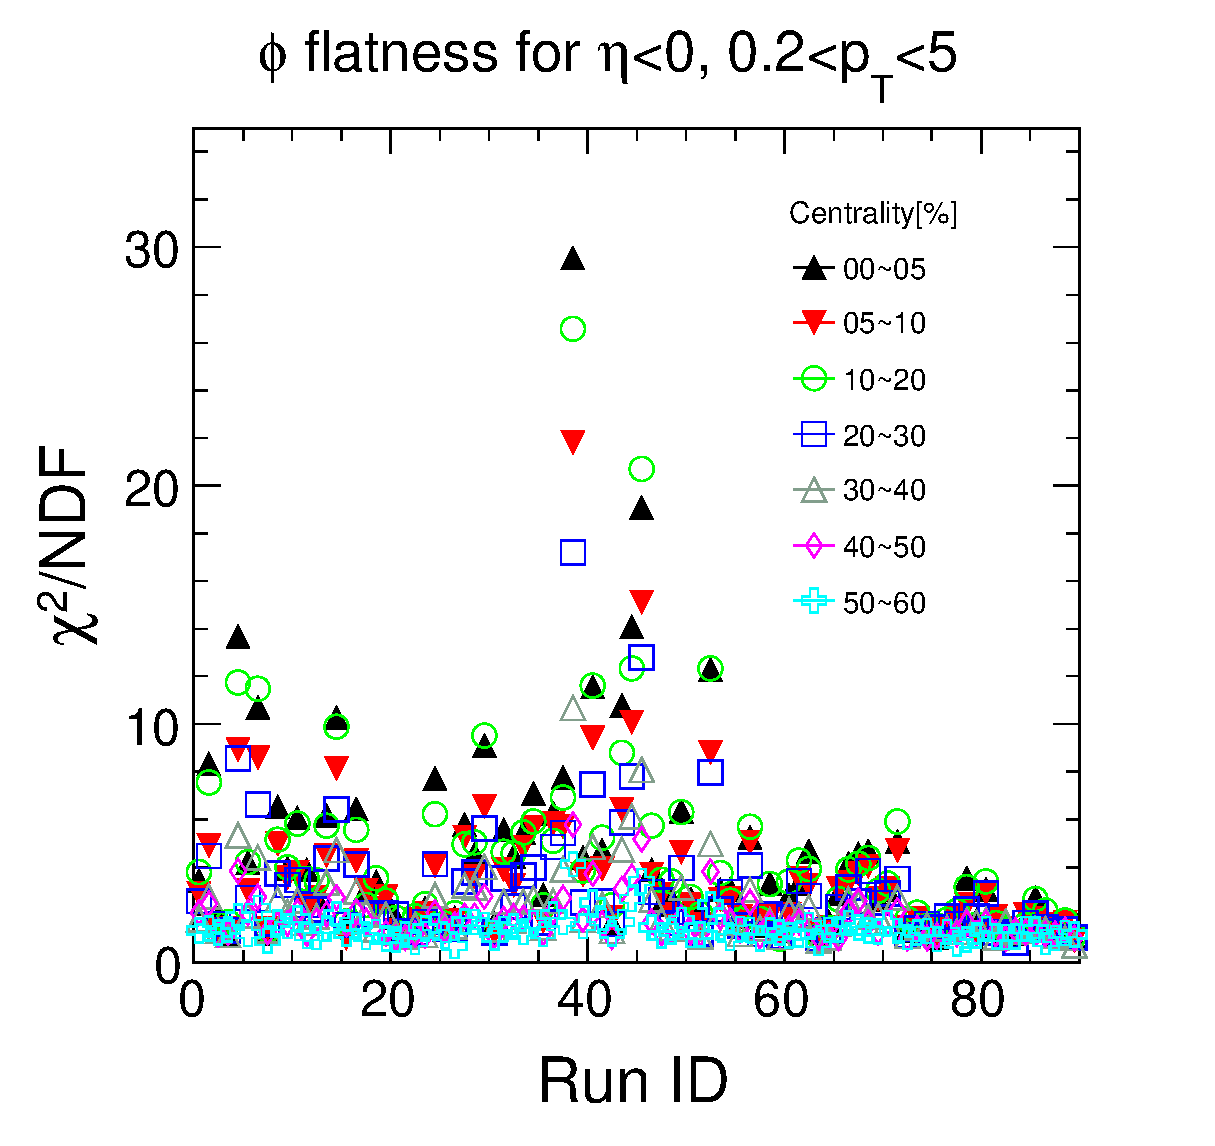
\includegraphics{figures/figs_QA/QA_RbR_phi_Aside_LHC10h_AOD86.eps}}
        	\resizebox{0.45\columnwidth}{!}{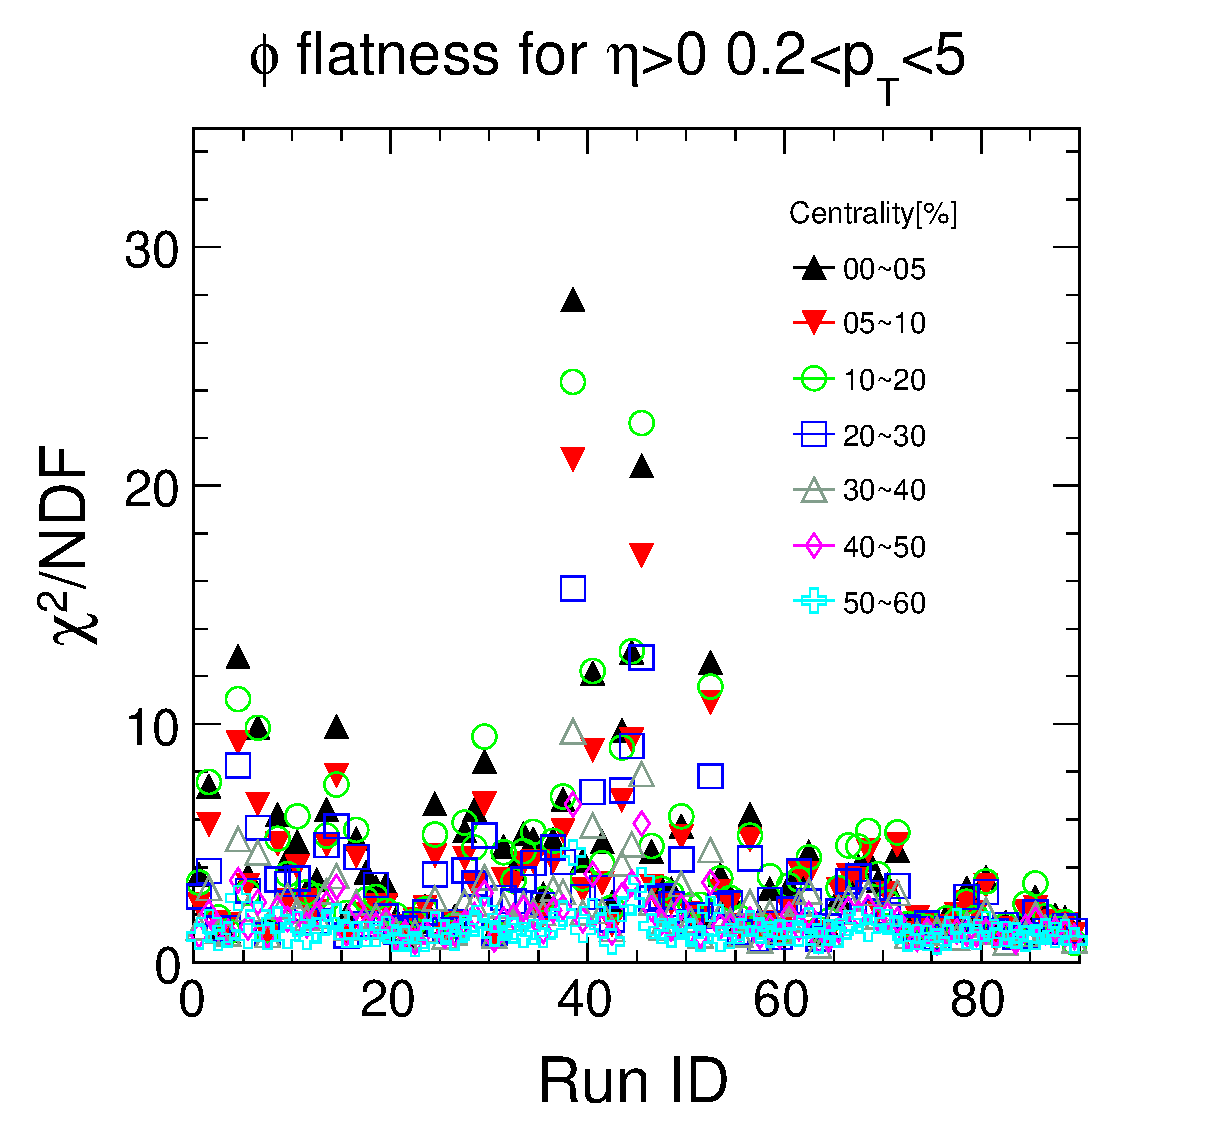
\includegraphics{figures/figs_QA/QA_RbR_phi_Cside_LHC10h_AOD86.eps}}
        \caption{$\chi^2/NDF$ for $\phi$ flatness for $\eta < 0$(left) and $\eta > 0$(right)}
        \label{fig:QC_phi_chi2NDF}
        \end{center}   
     \end{figure}

As shown in the figure, the flatness ($\chi^2/NDF$ of $\phi$) of some runs is worse than others. This is  considered as a detector effect, and might be affect on our analysis. The effect of these non-uniform $\phi$ distribution will be treated as systematics and will be covered in systematic chapter.
 

\clearpage

\section{Analysis strategy}
\label{sec:analysis}


While from existing measurements an estimate can be placed on the average value of QGP's $\eta/s$, both at RHIC and LHC energies, what remains completely unknown is how the $\eta/s$ of QGP depends on temperature ($T$). This study has been just initiated by the theorists in Ref.~\cite{Niemi:2015qia}, where the first (and only rather qualitative) possibilities where investigated (see Fig.~1 therein). The emerging consensus of late is that it is unlikely that the study of individual flow harmonics $v_n$ will reveal the details of $\eta/s(T)$ dependence. In fact, in was demonstrated already in the initial study~\cite{Niemi:2015qia} that different $\eta/s(T)$ parameterizations can lead to the same centrality dependence of individual flow harmonics. In Ref.~\cite{Niemi:2012aj} new flow observables were introduced by the theorists, which quantify the degree of correlation between two different harmonics $v_m$ and $v_n$. The initial success of these new observables was attributed to their potential to discriminate for the first time the two respective contributions to anisotropic flow development---from initial conditions and from the transport properties of the QGP~\cite{Niemi:2012aj}. Therefore their mesurement in turn would enable the experimental verification of theoretical predictions for individual stages of heavy-ion evolution independently. Besides this advantage, it turned out that correlations of different flow harmonics are sensitive to the details of $\eta/s(T)$ dependence~\cite{ALICE:2016kpq}, to which individual flow harmonics are nearly insensitive~\cite{Niemi:2015qia}. 

 For technical reasons, discussed in detail in Refs.~\cite{ALICE:2016kpq,Bilandzic:2013kga}, the correlations between different flow harmonics cannot be studied experimentally with the same set of observables introduced by the theorists in Ref.~\cite{Niemi:2012aj}. Instead, in~\cite{Bilandzic:2013kga} the new flow observables obtained from multiparticle correlations, so-called \textit{Symmetric Cumulants~(SC)}, were introduced to quantify in the most realiable way (i.e. nearly insensitivy to nonflow) the correlation of amplitudes of two different flow harmonics. The technical details are elaborated in Ref.~\cite{Bilandzic:2013kga}, while the first measurements of $SC$ observables were recently released by ALICE Collaboration in Ref.~\cite{ALICE:2016kpq}. For the convention, we will denote \textit{Symmetric Cumulants} for $m$th order and $n$th order as $SC(m,n)$ from now on.  This new observable are based on 4-particle cumulant, and defined as 

\begin{eqnarray}
	SC(m,n) &=&  \langle\langle \cos(m\varphi_1 + n\varphi_2 - m\varphi_3 - n\varphi_4 \rangle \rangle \nonumber \\ 
		&&- \langle \langle \cos{[m(\varphi_1 - \varphi_2)]} \rangle \rangle \langle \langle \cos{[n(\varphi_1 - \varphi_2)]} \rangle \rangle  \\ 
	  &=& \langle v_n^2 v_m^2 \rangle - \langle v_n^2 \rangle \langle v_m^2 \rangle \label{eq:SC}
\end{eqnarray}
\smallskip
 where double angular brackets indicates that the averaging has been extended from single to all events. Due to the condition that $m \neq n$, a lot of terms which appear in the general cumulant expansion are non-isotropic and  therefore, average to zero for a detector with uniform acceptance when the averaging is extended to all events. 
 
 
 These values can be obtained by multi-particle correlation with q-Cumulants such as 
 
\begin{equation}
	\langle \langle 2 \rangle \rangle \equiv \langle \langle e^{in(\phi_1 - \phi2)} \rangle \rangle \equiv \frac{\sum_{i=1}^{N}{(W_{\langle 2 \rangle})_i}\langle 2 \rangle_2 }{\sum_{i=1}^{N}{(W_{\langle 2 \rangle})_i}}
	\label{eq:2pcorr}
\end{equation}
\begin{equation}
	\langle \langle 4 \rangle \rangle \equiv \langle \langle e^{in(\phi_1 + \phi_2 - \phi_3 - \phi_4)} \rangle \equiv \frac{\sum_{i=1}^{N}{(W_{\langle 4 \rangle })_i}\langle 4 \rangle_i }{\sum_{i=1}^{N}{(W_{\langle 4 \rangle})_i}}
\end{equation}
\smallskip

The choice for the event weights in above equations is not arbitrary and we will outline in Appendix D. It has a physical meaning which will render the number of combinations (i.e. number of distinct 2- and 4-particle combinations one can form for an event with multiplicity M) as the only correct event weight.
 
 For fixed value of $v_n$ and $v_m$ over all events, the $SC(m,n)$ which defined as like Eq.\ref{eq:SC}, is zero by definition. Moreover we can obtain the result in the last line of above equation not only when $v_m$ and $v_n$ are fixed for all events, but also when event-by-event fluctuations of $v_m$ and $v_n$ are correlated( or anti-correlated).
 
This $SC(m,n)$ is very efficient observables for measuring flow ``magnitude" correlation because it's free from event-plane which is directly related to ``direction" correlation. (Any dependence on the event plane $\psi_n$ and $\psi_m$ is canceled by definition) 

As a result, the Eq.\ref{eq:SC} holds, the correlation between flow harmonics, and we can concluded whether finding $v_m$ larger than $\langle v_m \rangle$ in an event will enhance(or reduce) the probability of finding $v_n$ larger than $\langle v_n \rangle$ in that event. 

In this analysis, we are going to show $SC(m,n)$ results which can be calculated for correlation between flow harmonics by using 4- particle cumulants. In addition, we will show not only $SC(m,n)$ but also going to show  \textit{normalized} $SC(m,n)$ (also denote as $NSC(m,n)$)

\begin{eqnarray}
 NSC(m,n) &=& \frac{SC(m,n)}{\langle v_n^2 \rangle \langle v_m^2 \rangle } 	
 \label{eq:nSC}
\end{eqnarray}
\smallskip

\textit{Normalized symmetric cumulants} (NSC)  reflect only the degree of the correlation which is expected to be insensitive to the magnitudes of $v_{m}$ and $v_{n}$, while $SC(m,n)$ contains both the degree of the correlation and individual $v_{n}$ harmonics. In Eq.\ref{eq:nSC} the products in the denominator are obtained with two-particle correlations and using a psedorapidity gap of $|\Delta\eta|>1.0$ to suppress biases from few-particle nonflow correlations. On the other hand, in the two two-particle correlations which appear in the definition of $SC(m,n)$ the psedorapidity gap is not needed, since nonflow is suppressed by construction in \textit{SC observable}, as the study based on HIJING model has clearly demonstrated in Ref.~\cite{ALICE:2016kpq}.

However,  note that the following Eq.\ref{eq:nSC_1} and \ref{eq:nSC_2} are not held in this analysis because of the difference between products $\langle v_m^2 \rangle \langle v_n^2 \rangle$ for denominator and numerator. For the numerator, since nonflow is suppressed by construction in $SC(m,n)$ we do not apply any pseudorapidity($\eta$) gap for calculate 4- particle cumulants for all the particles in $|\eta| < 0.8$. But for the denominator, these products were obtained in ALICE with 2- particle correlations separately with using a pseudorapidity gap of $|\Delta \eta| >  1.0$ to suppress biases from few particle non-flow correlations. However, other theoretical studies \cite{Giacalone:2016afq} use both Eq.\ref{eq:nSC} and \ref{eq:nSC_2} for the  $NSC(m,n)$


\begin{eqnarray}
 NSC(m,n) &=& \frac{SC(m,n)}{\langle v_n^2 \rangle \langle v_m^2 \rangle } \nonumber \\ &=& \frac{ \langle  v_n^2 v_m^2 \rangle  - \langle v_n^2 \rangle \langle v_m^2 \rangle }{\langle v_n^2 \rangle \langle v_m^2 \rangle } \label{eq:nSC_1} \\ &=&   \frac{ \langle  v_n^2 v_m^2 \rangle   }{\langle v_n^2 \rangle \langle v_m^2 \rangle   }   -1	 \label{eq:nSC_2}
\end{eqnarray}


The $SC(m,n)$ provide orthogonal information to recently measured symmetry plane correlators in Refs.~\cite{ALICE:2011ab,Adare:2011tg,Aad:2014fla}. This statement does not exclude the possibility that both set of observables can be sensitive to the same physical mechanisms. In the recent theoretical study~\cite{Giacalone:2016afq} it was pointed out that the mechanism giving rise to symmetry plane correlations (nonlinear coupling) can also contribute to symmetric cumulants. As a concrete example it was discussed that the existing correlation due to hydrodynamic evolution between $V_4$ and $V_2^2$ (which are vectors in the transverse plane) implies that both the angles and the magnitudes are correlated~\cite{Giacalone:2016afq}. 

Interpretation of flow results obtained with multiparticle correlation techniques in small colliding systems, like pp and p--Pb at LHC, remains a challenge. The underlying difficulty stems from the fact that when anisotropic flow harmonic $v_n$ is estimated with $k$-particle correlator, the statistical spread of that estimate scales to leading order as $\sigma_{v_{n}}\sim\frac{1}{\sqrt{N}}\frac{1}{M^{k/2}}\frac{1}{v_{n}^{k-1}}$, where $M$ is the number of particles in an event (multiplicity) and $N$ is total number of events. This generic scaling ensures that multiparticle correlations are precision method only in heavy-ion collisions, characterized both with large values of multiplicity and flow. To leading order the measurements in small systems~\cite{Aad:2013fja,Abelev:2014mda,Khachatryan:2015waa,Adamczyk:2015xjc,Adare:2015ctn} and the measurements in heavy-ion collisions resemble the same features, which can be attributed to collective anisotropic flow in both cases. However, such interpretation is challenged by the outcome of recent Monte Carlo study~\cite{Loizides:2016tew} for $e^+e^-$ systems in which collective effects are not expected. Nonetheless, in this study to leading order multiparticle correlations exhibit yet again the similar universal trends first seen in heavy-ion collisions, both for elliptic and triangular flow. Therefore, it seems unlikely that the analysis of individual flow harmonics with multiparticle techniques will answer whether collective effects can develop and QGP be formed in small systems---instead new observables, like SC, might provide the final answer due to their better sensitivity~\cite{Niemi:2012aj,ALICE:2016kpq}.



\subsubsection{Measuring $SC(m,n)$ with Scalar Product method}
In this analysis, we are going to show that $SC(m,n)$ also can be calculated  by the Scalar Product(SP) method via measuring moments \cite{Bhalerao:2015jg} with single $\eta$ gap. By introducing single $\eta$ gap between two different sub-event group can avoid auto (self)-correlation and can suppress non-flow effects. To calculate SC(m,n) with the SP method, we need to define the (normalized) flow Q-vector such as

\begin{equation}
	 Q_n = \frac{1}{N} \sum{e^{in\varphi}  } 
\end{equation}

Then, the flow magnitude can be easily obtained with $Q$-vector calculation. 

\begin{equation}
	\langle v_n^{2k} \rangle  = \langle V_n^{k*} V_n^k\rangle= \langle Q_{nA}^{*k} Q_{nB}^k \rangle
\end{equation}

To avoid self-correlation when calculating $v_n^2$, we divide particles into 2 sub event groups and introduced single $\eta$ gap between sub event group to suppress non-flow effect. So main difference between original method and this method is that calculate correlation with full-particle $Q$-vector or divided-particle $Q$-vector, and existence of $\eta$ gap around 0. 

\begin{eqnarray}
\langle v_m^2 v_n^2 \rangle - \langle v_m^2 \rangle \langle v_n^2 \rangle 
 &=& \langle V_n V_n^{*} V_m V_m^{*}\rangle - \langle V_n^k V_n^{*} \rangle \langle V_m^k V_m^{*}\rangle \\ 
 &=& \langle {Re( Q_{An} Q_{Bn}^* Q_{Am} Q_{Bm}^*)} \rangle - \langle {Re( Q_{An}Q_{Bn}^*) } \rangle  \langle { Re(Q_{Am} Q_{Bm}^*) }\rangle \nonumber \\  
\end{eqnarray}


In this analysis, we take denotation ``A" for sub-event group which have negative $\eta$ range ( $-0.4 > \eta > -0.8$ ) and ``B" for positive $\eta$ range ( $0.4 < \eta < 0.8$ ). Because we divided into 2 sub groups, particles will not count twice when calculating $Q_{An} Q_{Bn}^*$, but there are still possible of auto (self) correlation when calculating ``$Q_{An} Q_{Bn}^* Q_{Am} Q_{Bm}^*$", this effect is probably small but can be corrected with the analytical method. 

\begin{equation}
	v_n^{2k}v_m^{2l} = \langle  Q_{nA}^{*k} Q_{nB}^k Q_{mA}^{*k} Q_{mB}^k \rangle
\end{equation}

The auto correlation during above the equation happens because there is a $\eta$ gap between $Q_{nA}^{*k} Q_{nB}^k$, and $Q_{mA}^{*k} Q_{mB}^k$ but not between $Q_{nA}^{*k}Q_{mA}^{*k}$ nor $Q_{nB}^k Q_{mB}^k$,  the auto (self) correlation effect can be corrected by changing equation of $SC(m,n)$ from

\begin{equation}
	\langle {Re( Q_{An} Q_{Bn}^* Q_{Am} Q_{Bm}^*)} \rangle - \langle {Re( Q_{An}Q_{Bn}^*) } \rangle  \langle { Re(Q_{Am} Q_{Bm}^*) }\rangle 
\end{equation}
to

\begin{equation}
\begin{split}
	\langle &Re( Q_{An} Q_{Bn}^* Q_{Am} Q_{Bm}^*) - \frac{1}{M_B} Re(Q^*_{Bm+n}Q_{Am}Q_{An})\\
	 &-\frac{1}{M_A}Re(Q_{Am+n}Q^*_{Bn}Q^*_{Bm}) + \frac{1}{M_A M_B}Re(Q_{Am+n}Q^*_{Bm+n}) ) ) \rangle  \\
	 &- \langle {Re( Q_{An}Q_{Bn}^*) } \rangle  \langle { Re(Q_{Am} Q_{Bm}^*) }\rangle
\end{split}		
\end{equation}

	\begin{figure}[h]
		\begin{center}
     	   	\resizebox{0.45\columnwidth}{!}{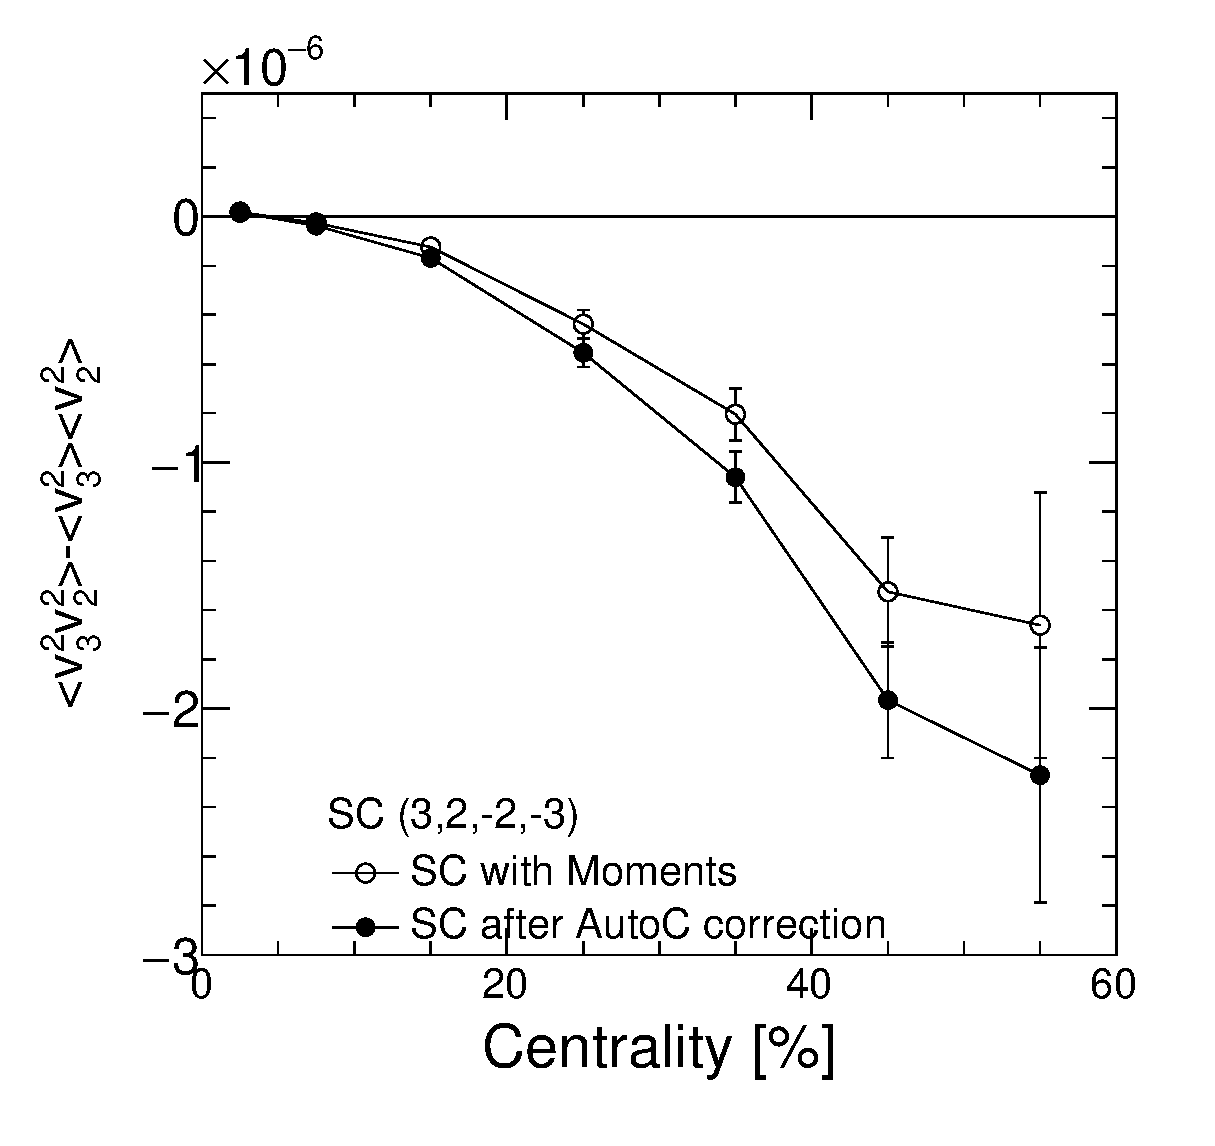
\includegraphics{figures/figs_SCpt/SC_LHC10h_3223_compare}}
              	\resizebox{0.45\columnwidth}{!}{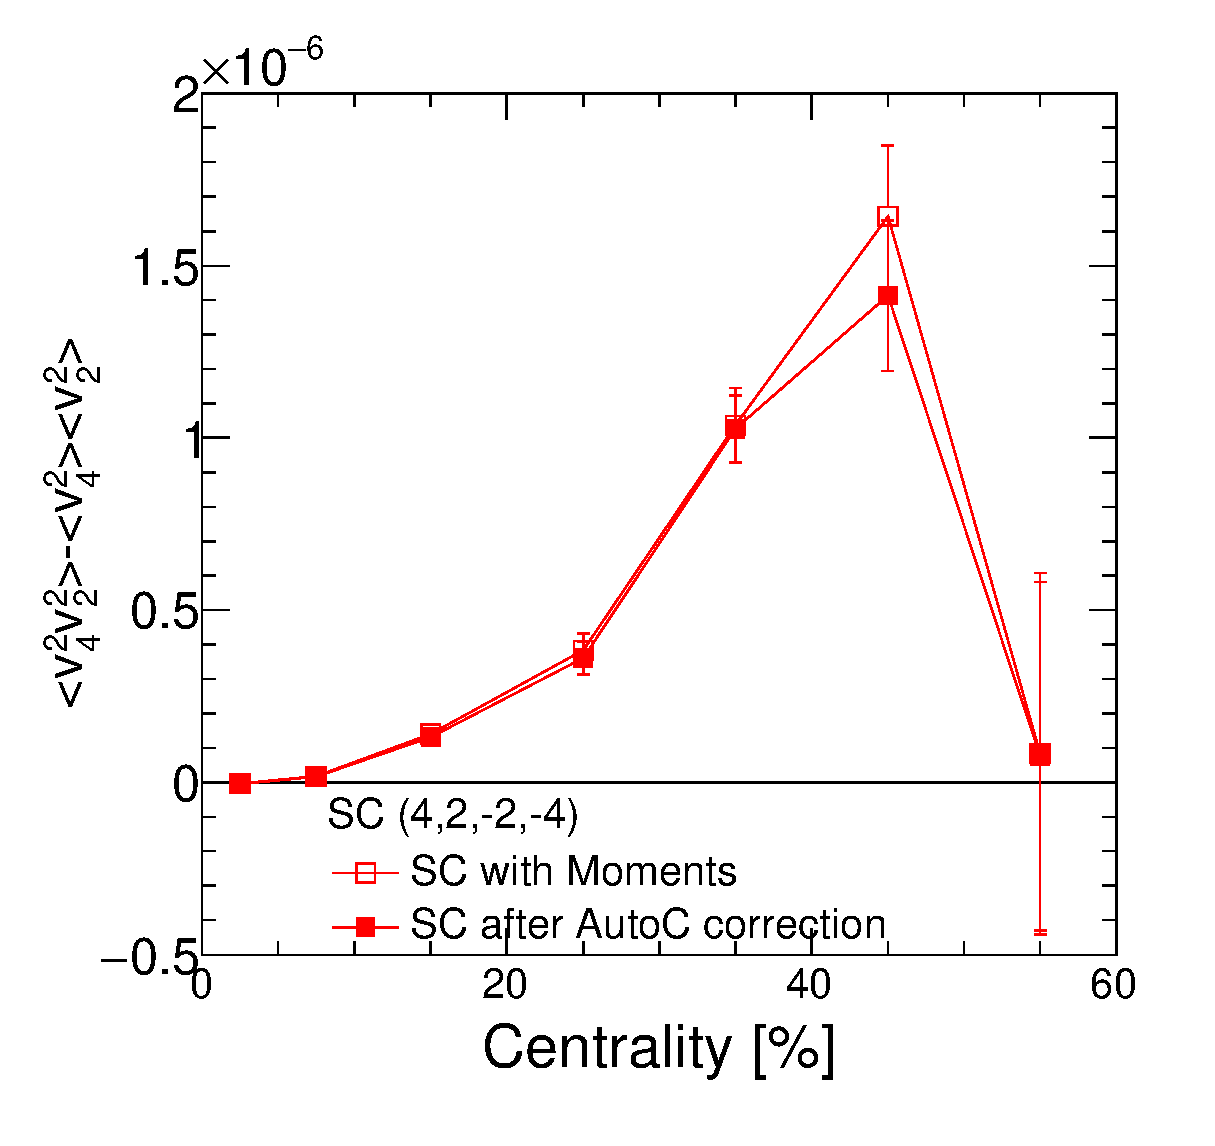
\includegraphics{figures/figs_SCpt/SC_LHC10h_4224_compare}}
        \label{SC42_autoC}
        \caption{Results of $SC(3,2)$(left) and $SC(4,2)$ before auto (self)-correlation correction(open makers) and after correction(closed markers)}
        \end{center}   
     \end{figure}




\vskip15mm

The detailed results of $SC(m,n)$ and  $NSC(m,n)$ with various flow harmonics, and comparison with hydrodynamic calculations and MC simulations, and also the $p_T$ dependence of $SC(m,n)$ and $NSC(m,n)$ and the difference between two different measuring method (QC vs SP) will be covered in the results chapter.

\section{Systematics}

	In this section, the systematic uncertainties of $SC(m,n)$ and  $NSC(m,n)$ will be presented. The systematic uncertainties were estimated by varying the event and track selection criteria. All systematic checks described here are performed independently. Each results of $SC(m,n)$ (and also $NSC(m,n)$) with a selected criterion are compared to ones from the default event and track selection described in the previous chapter. The differences between the default results and the ones obtained from the variation of the selection criteria are taken as systematic uncertainty of each individual source.
The different ratio were fitted with a 0-th order polynomial as function of centrality to suppress point-to-point statistical fluctuations and to extract the overall systematics. The contributions from different sources were then merged in quadrature to obtain the final value of the systematic uncertainty. The detailed conditions varying for systematics studies were described in the following.
	
	
	
\subsection{Systematics from Non uniform phi distribution}
	
	
This section is about systematics uncertainty from the non-uniform efficiency of detector performance. In principle, the $\phi$ distribution of produced particle should be flat over all events unless detector effect. But in our data, as seen in the previous section in data QA (see figure.\ref{fig:QC_phi_chi2NDF}), the distribution of the transverse angle of particle produced is not perfectly uniform due to detector effects like inefficiency or dead-zone area. And these non-uniform $\phi$ distributions vary run-by-run, and it is not easily corrected by simple weight correction for specific $\phi$ angle.

 This non-uniform $\phi$ distribution might change the final results of $SC(m,n)$ and should be taken into systematic uncertainty. The simplest and basic approach to check the effect of non-uniform distribution is categorize run groups into two sub groups to have good $\phi$ distribution, and for the other group to have bad $\phi$ distribution. Then measure the $SC(m,n)$ values with each sub groups independently and calculated the difference between them as the systematic uncertainty. However, to use this methods, we need to have almost same number of events for each groups. Even though we have similar number of events for each groups, we are going to have larger statistical error because of half of events in this way. 

  In this analysis, to check systematic uncertainties from non-uniform $\phi$ distribution, we use AMPT simulation which has better match to data than any other existing models. We measure $SC(m,n)$ with the large statistics AMPT dataset which has  flat $\phi$ distribution, and impose non-uniform $\phi$ distribution from data and calculate the difference between original AMPT and modified AMPT as systematic uncertainty from non-uniform $\phi$ distribution. 


 	\begin{figure}[h]
		\begin{center}
        	\resizebox{0.85\columnwidth}{!}{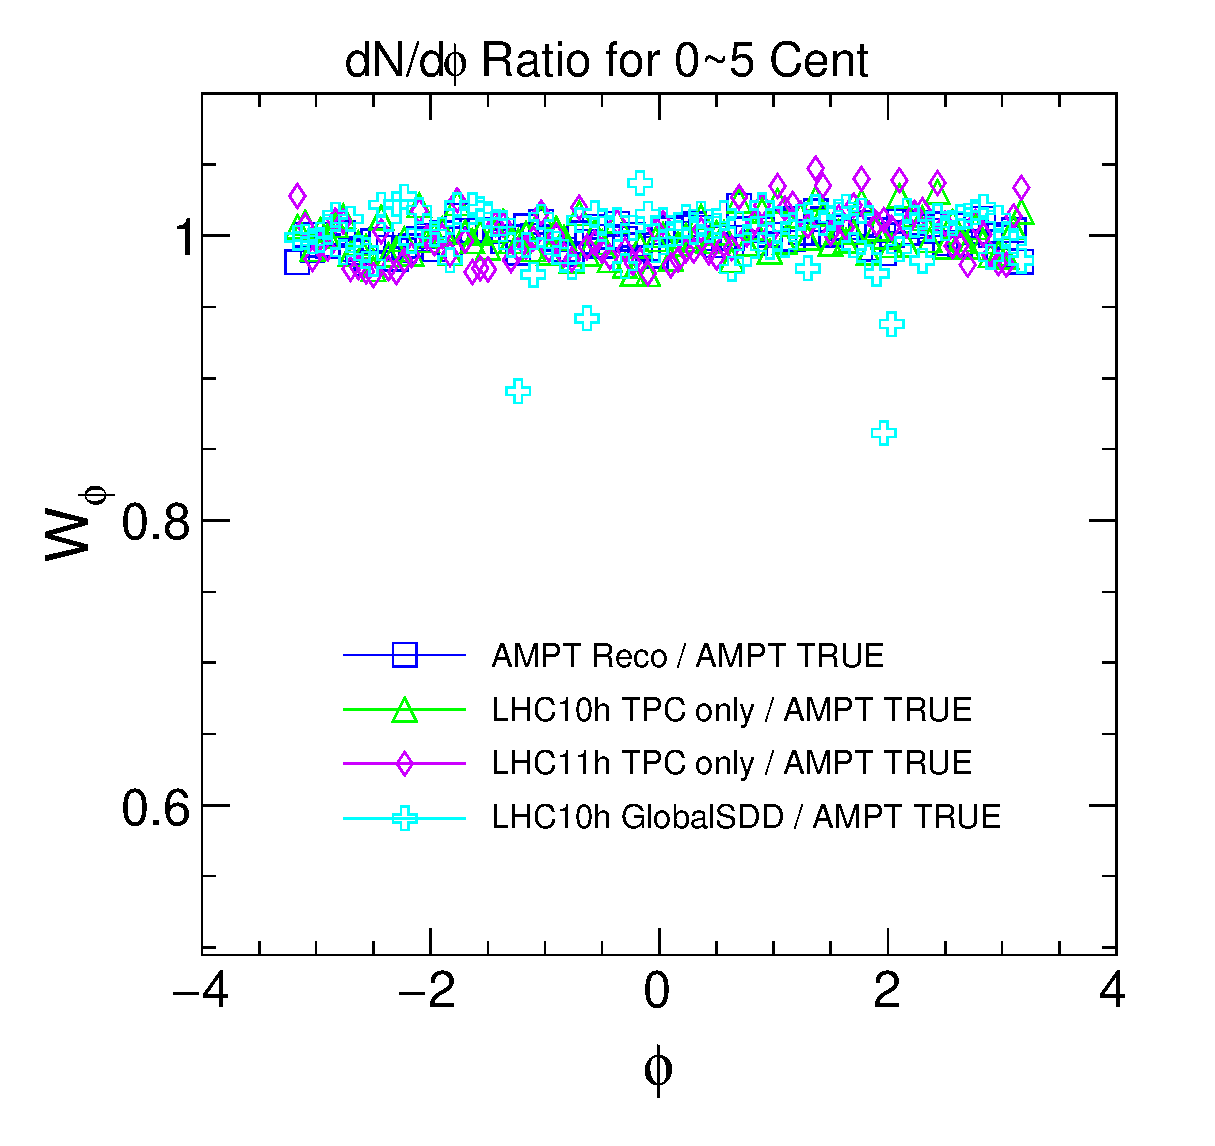
\includegraphics{figures/figs_QA/impose_NUE.eps}}
        \caption{Scaled ratio of $dN/d\phi$ distribution of ALICE LHC10h dataset to flat distribution (AMPT True). The reconstructed AMPT, and LHC11h with TPC only track cut, and LHC10h with Global SSD track cut were also drawn together for comparison.}
        \label{fig:QC_impose}
        \end{center}   
     \end{figure}
	
The non-uniform $\phi$ distribution which is taken from ALICE LHC10h data are shown in Fig.\ref{fig:QC_impose}. We use TPC only track cut, which have better $\phi$ distribution, but also LHC10h with Global SDD and LHC11h distribution were shown together for comparison. As seen in figure, the data from LHC10h period have worse flatness than AMPT simulation. It becomes even worse in GlobalSSD track cut or LHC11h period data because of some detector problems. (Some of SDD clusters in ITS detector were dead in 2010, and there was reconstruction efficiency issue with TPC detector in 2011 data taking) The results with AMPT data and modified AMPT data were calculated together and the difference between them was taken into systematic uncertainties. 


	\subsection{Systematics from Event selection}
	
	Following is the list of item for systemic uncertainty study about event selections. 
	
\subsubsection{Z-vertex cut}

Because of limited acceptance of ALICE detector, primary vertex position along the longitudinal direction is important to ensure for the uniform pseudo-rapidity distribution over all events. The z-vertex distribution of ALICE LHC10h events are shown in Fig.\ref{fig:zvtx}.  As described in previous chapter, the reconstructed vertex position in beam axis (z-vertex) is required to be located within 10 cm of interaction point (IP). Since  the different z-vertex position may have an effect on effective $\eta$ range. So these Z-vertex cut criteria are important to ensure for the flat $\eta$ distribution over all events. 	Instead of using the original vertex range cut ($|z| < 10$ cm),  we tried to reduce $|z| < 8$ cm for systematic study.	
		
 	\begin{figure}[h]
		\begin{center}
        	\resizebox{0.65\columnwidth}{!}{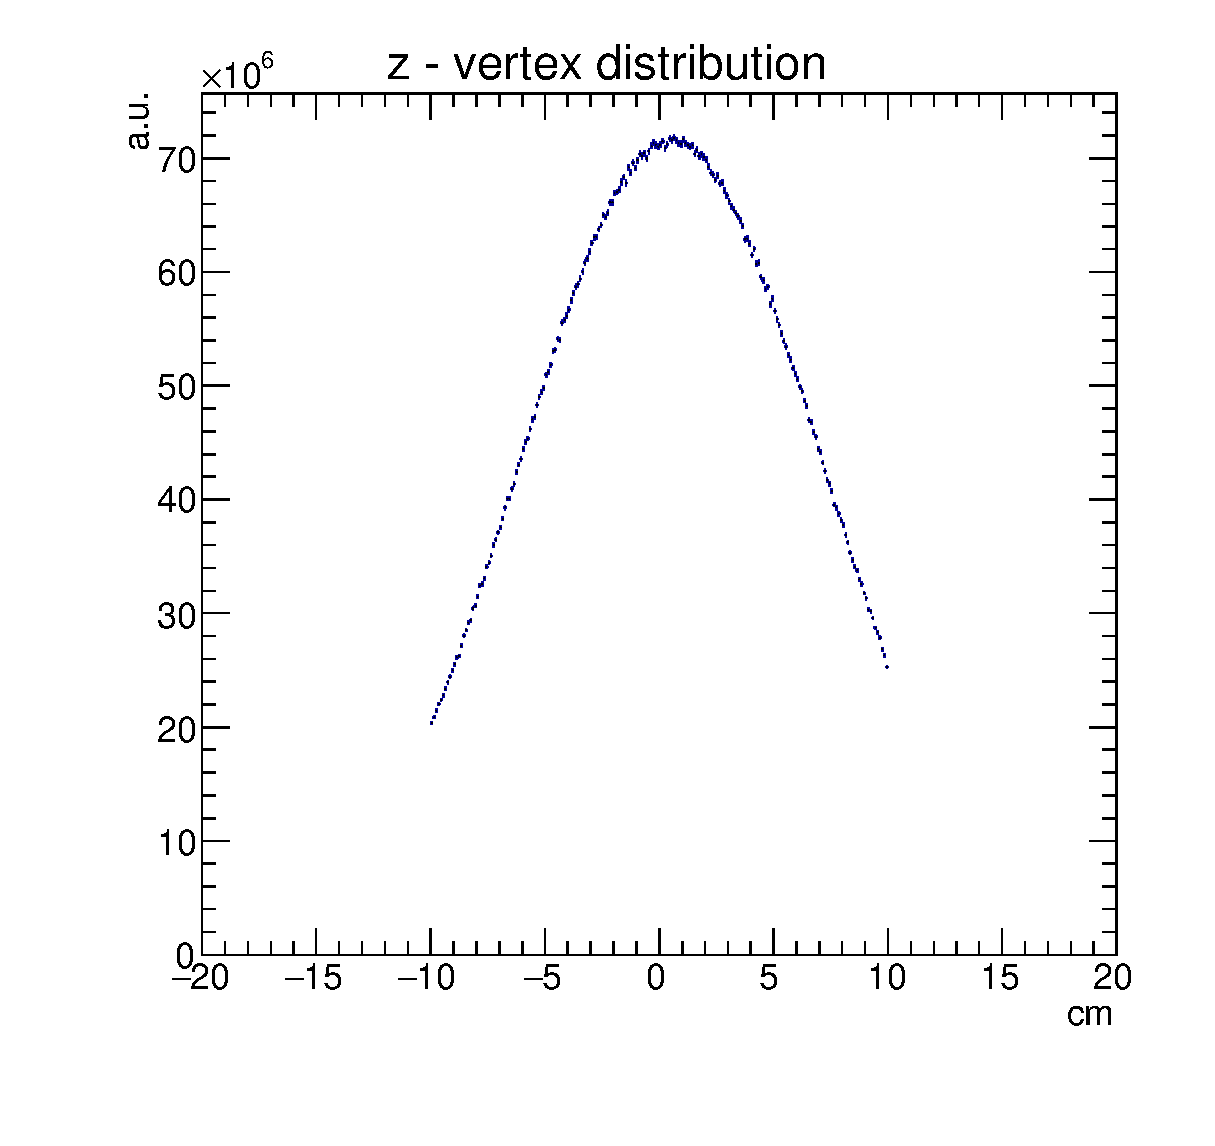
\includegraphics{figures/figs_systematics/zvtx_dist}}
        \caption{Z-vertex distribution of ALICE Pb + Pb $\sqrt{S_{NN}} = 2.76$~TeV with minimum bias triggered events }
        \label{fig:zvtx}
        \end{center}   
     \end{figure}


	
\subsubsection{Magnetic polarization}
	The events which we analyzed were recorded with two settings of the magnetic field polarities, namely (++) and  (--). For the default, we used all the events from both polarized magnetic fields. The configuration of magnetic polarizations consist of almost the same number of events. We measured the $SC(m,n)$ results from (++) or (--) categorized events and compare to the default one.
	
\subsubsection{Centrality determination}
	The centrality of the given collision can be determined by various detectors and settings. By the default, the multiplicity of the VZERO detector(Both V0A and V0C) is used for centrality determinations with better than 2\% of resolution. Another method of determine event centrality were using the multiplicity of tracks estimated by the standalone TPC tracking or tracklet from SPD detector independently which have slightly worse resolution. We use these methods to study systematic uncertainty from centrality determination.
	
\subsubsection{Cut on outliers}
	The outlier is an observation point that is different from other observations. In LHC10h datasets, there are some events which have many more TPC tracks than Global reconstructed tracks. These outliers is coming from pile-up like events or indicate experimental error. These kind of outliers usually are discarded from the data sets. In these case, we excluded the events which have Multiplicity of TPC except following criteria	
	
	\begin{equation}
		32.1 + 1.59 \times M_{Global} < M_{TPC} < -40.3 + 1.22 \times M_{Global} 
	\end{equation}
	
		
 	\begin{figure}[h]
		\begin{center}
        	\resizebox{0.45\columnwidth}{!}{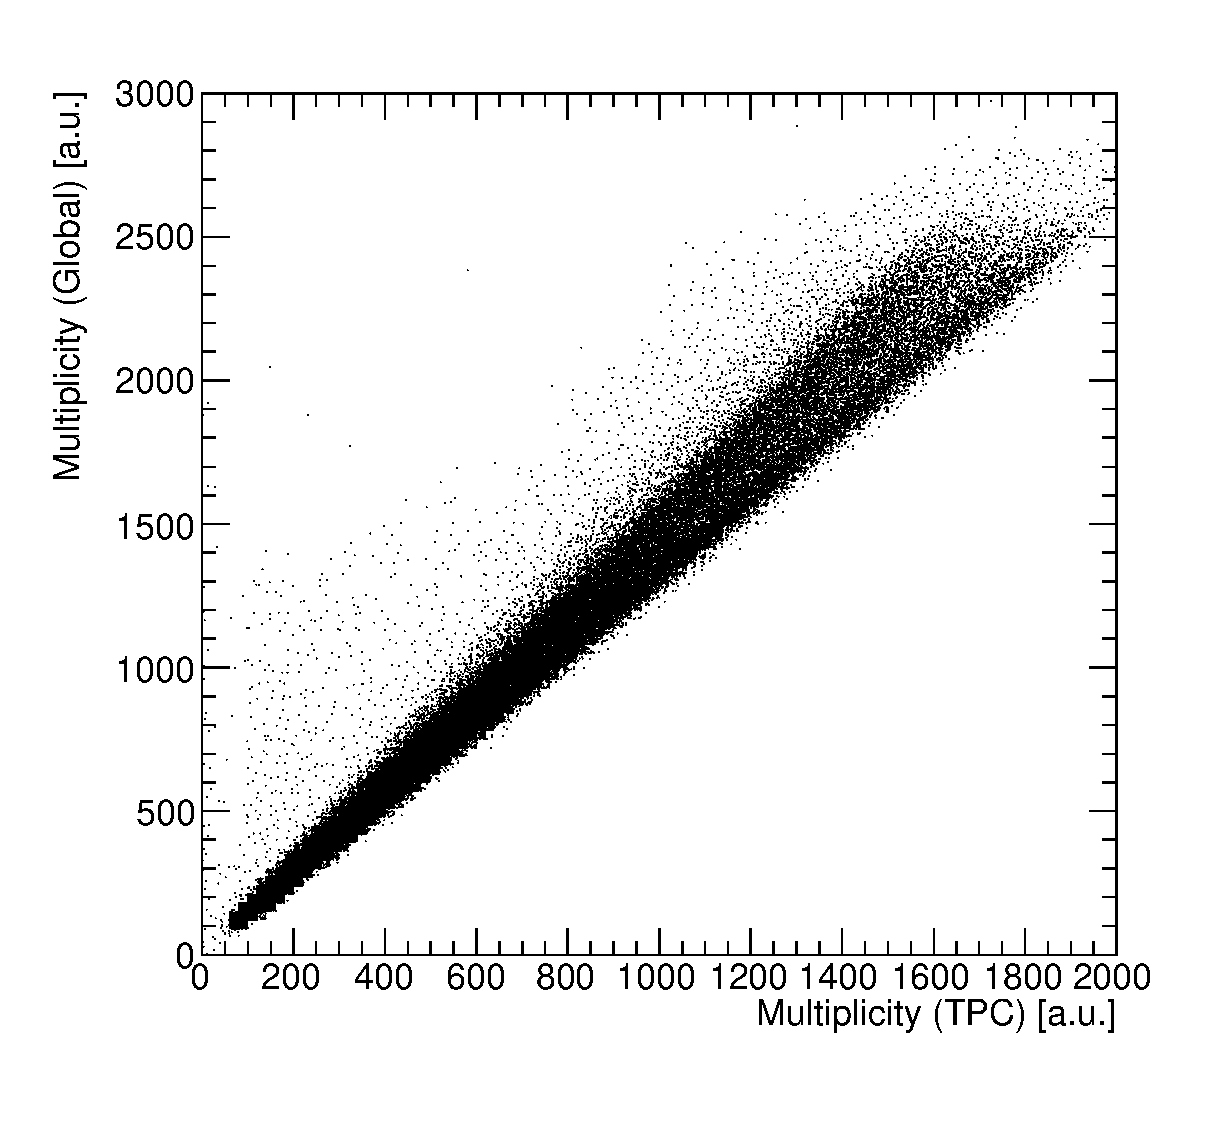
\includegraphics{figures/figs_systematics/outlier_off.eps}}
        	\resizebox{0.45\columnwidth}{!}{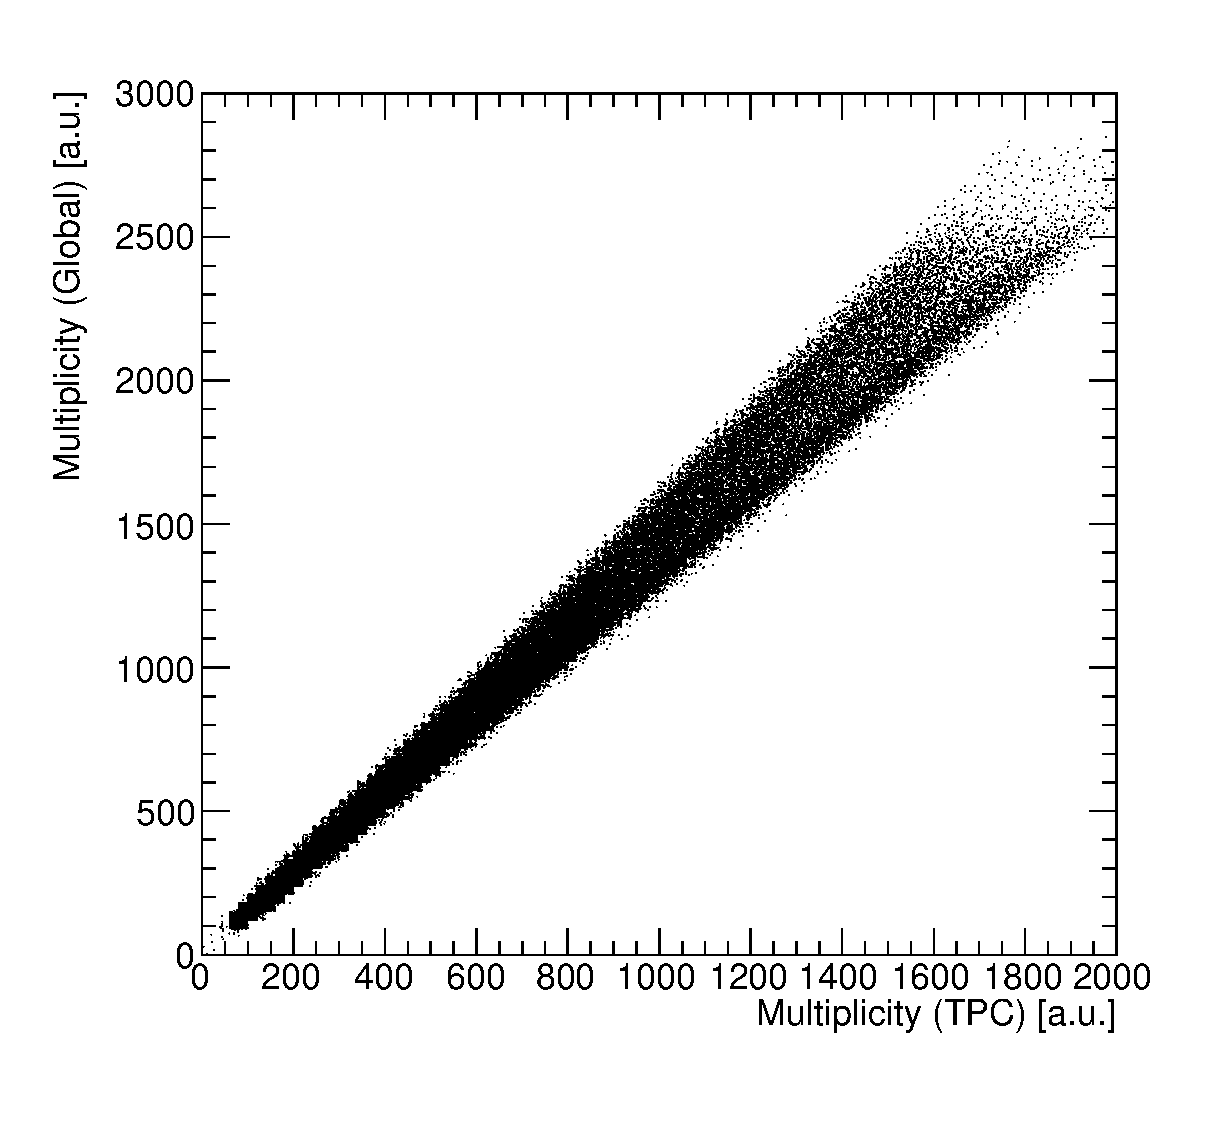
\includegraphics{figures/figs_systematics/outlier_on.eps}}
        \caption{The 2-dim distribution of TPC multiplicity and Global multiplicity. Left is the before exclude outlier(left) and right figure is after exclude outlier(right) events. }
        \label{fig:outlier}
        \end{center}   
     \end{figure}



\subsection{Systematics from Track selection}
	Following is the list of item for systematic uncertainty study form track selections.
	
\subsubsection{Track filter bit}
	As can see the Fig.\ref{fig:dndphi}, $\varphi$ flatness vary as track selection filter cuts, and it might affect the results of $SC(m,n)$ which is sensitive to $\phi$ distribution. This incompleteness of $\phi$ distribution comes from the limited precision with the detector performance. And each track filter cuts were evaluated by the thresholds on parameters used to select the tracks at the reconstruction level. Usually TPC only track cuts have relatively good(flat) $\phi$ distribution than GlobalSDD cut, but more fake and secondary tracks are included. Also GlobalSDD cut gives two small holes in $\phi$ distribution. 
			
 	\begin{figure}[h]
		\begin{center}
        	\resizebox{0.65\columnwidth}{!}{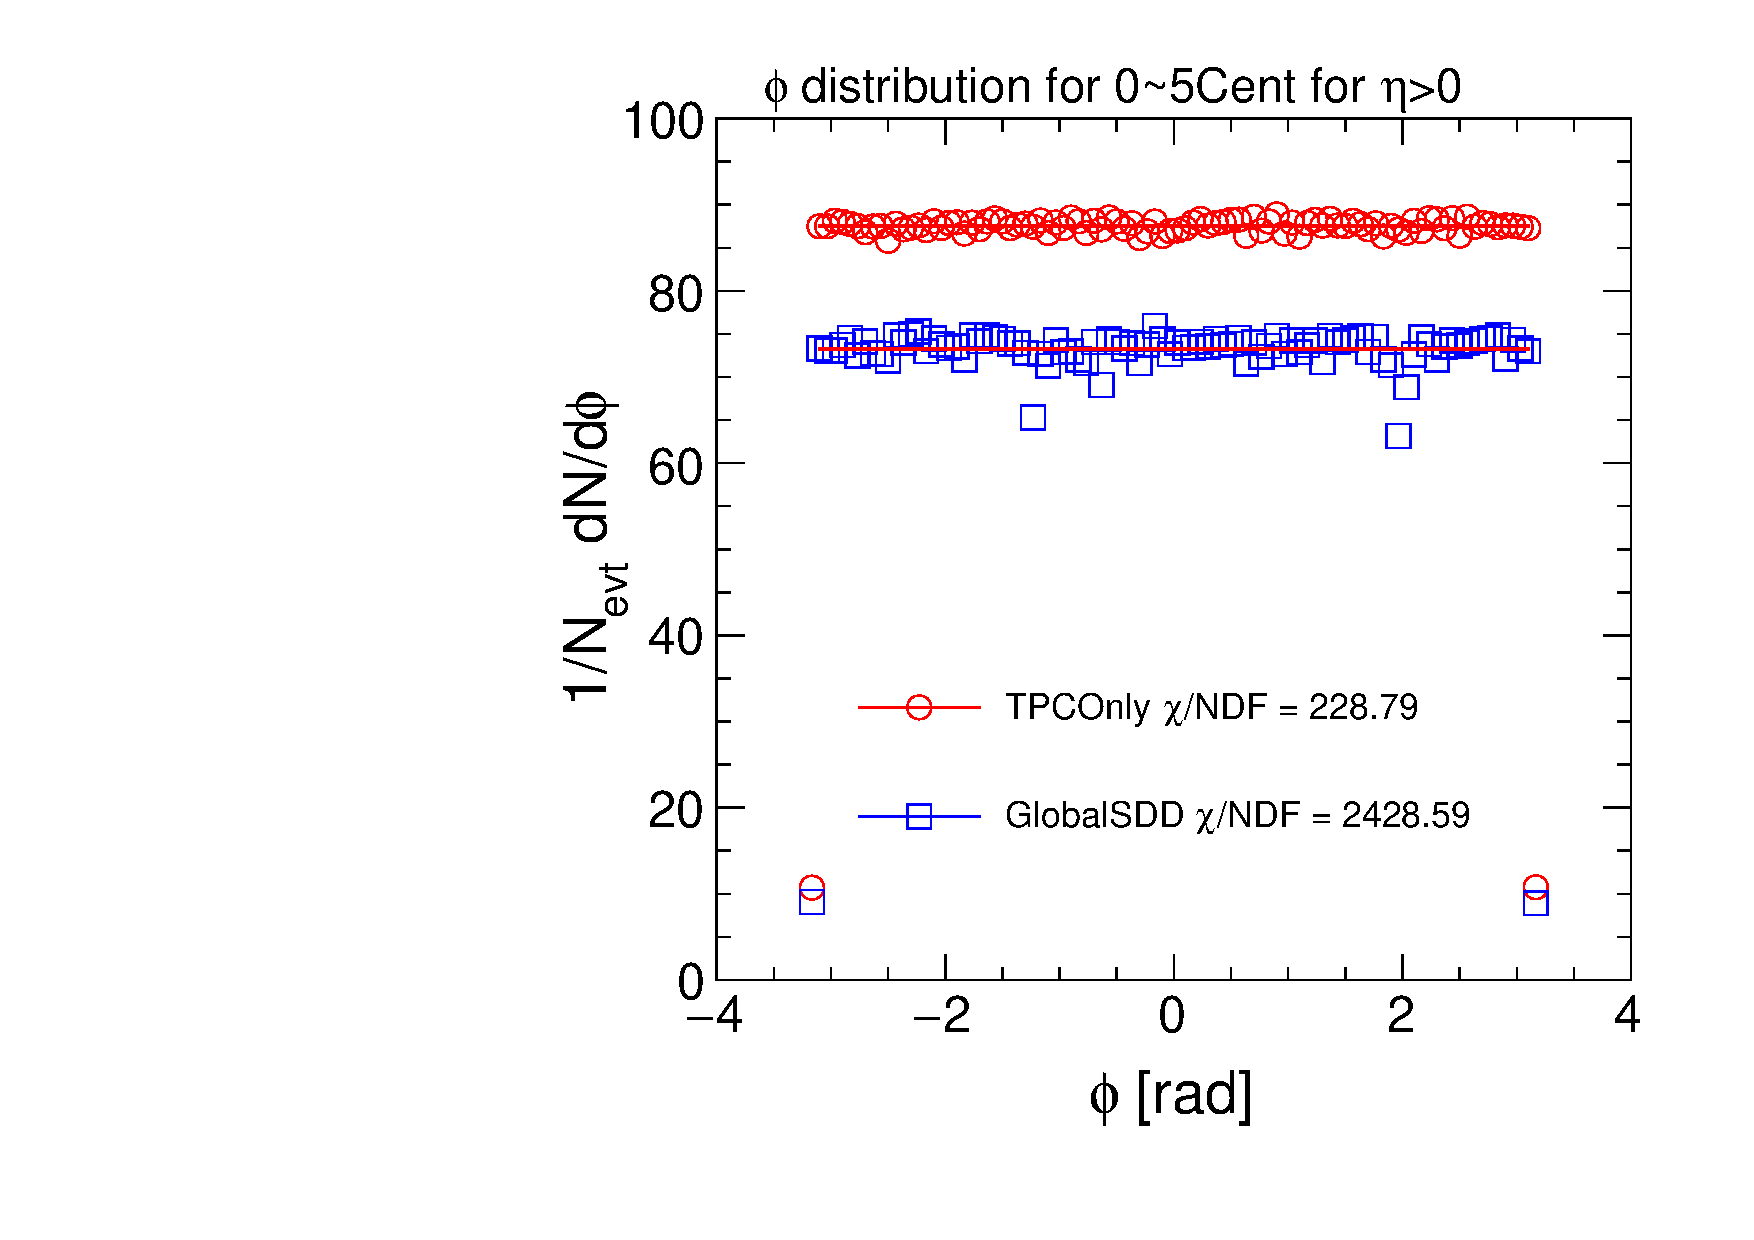
\includegraphics{figures/figs_systematics/dNdphi_TPCOnly_GlobalSDD_eta0_0}}
        \caption{$\chi/NDF$ of $dN/d\varphi$ distribution from ALICE LHC10h data with TPC only track selection filter and Global SDD filter.}
        \label{fig:dndphi}
        \end{center}   
     \end{figure}
	
\begin{table}[!h]
\begin{center}
\begin{tabular}{c|c|l}
\hline
cut		  & filter bit    & comments \\ \hline
TPCOnly   & 128 ( 7 )     & GetStandardTPCOnlyTrackCuts() \\
	      &               & + SetMinNClustersTPC(70)\\ \hline
GlobalSDD & 96  ( 5$|$6)  & GetStandardITSTPCTrackCuts2010()  \\ 
	      &               & with requiring the first SDD cluster \\ 
	      &               & instead of an SPD cluster \\ \hline
\end{tabular}
\caption{ALICE Track selection filter conditions}
\end{center}
\end{table}

To estimate systematic uncertainty from the track selection filter cut, we measure the results from different track selections and compare with the default setting.
	
	
\subsubsection{Charge combination}

We used 4p- and 2p- correlation to measure $SC(m,n)$. The multiparticle cumulants are expected to remove non-flow effect by cancellation each other, however it is hard to prove there is perfectly absense of non-flow effects in $SC(m,n)$. To estimate remain non-flow effects, such as re-reinteraction with other particles in the system after leaving the domain, the modification of the jet-like two-particle correlations, resonance decays, and final state interactions (particularly Coulomb effects).  Such flowing cluster contributes to cumulants by definition as being genuine four particle correlations, however, due to charge conservation, we will have in the cluster always particles of opposite charge. Therefore, by performing an independent analysis only with like-sign charges, we are estimating the contribution from flowing clusters. 



\subsubsection{Efficiency correction}

The correction to $p_T$ dependent efficiency were also tested, and taken into systematic uncertainty. Because of incompleteness of track reconstruction, correction steps are necessary to trace back from reconstructed tracks to the orignally generated particles from the collisions. Usually this study were conducted with a Monte Carlo simulation such as HIJING for Pb+Pb coliisions and PYTHIA for the $p$-$p$ collisions. The single track reconstruction efficiency, and contamination form the secondary particles were shown in FIg.\ref{fig:eff}

		
 	\begin{figure}[!p]
		\begin{center}
        	\resizebox{0.65\columnwidth}{!}{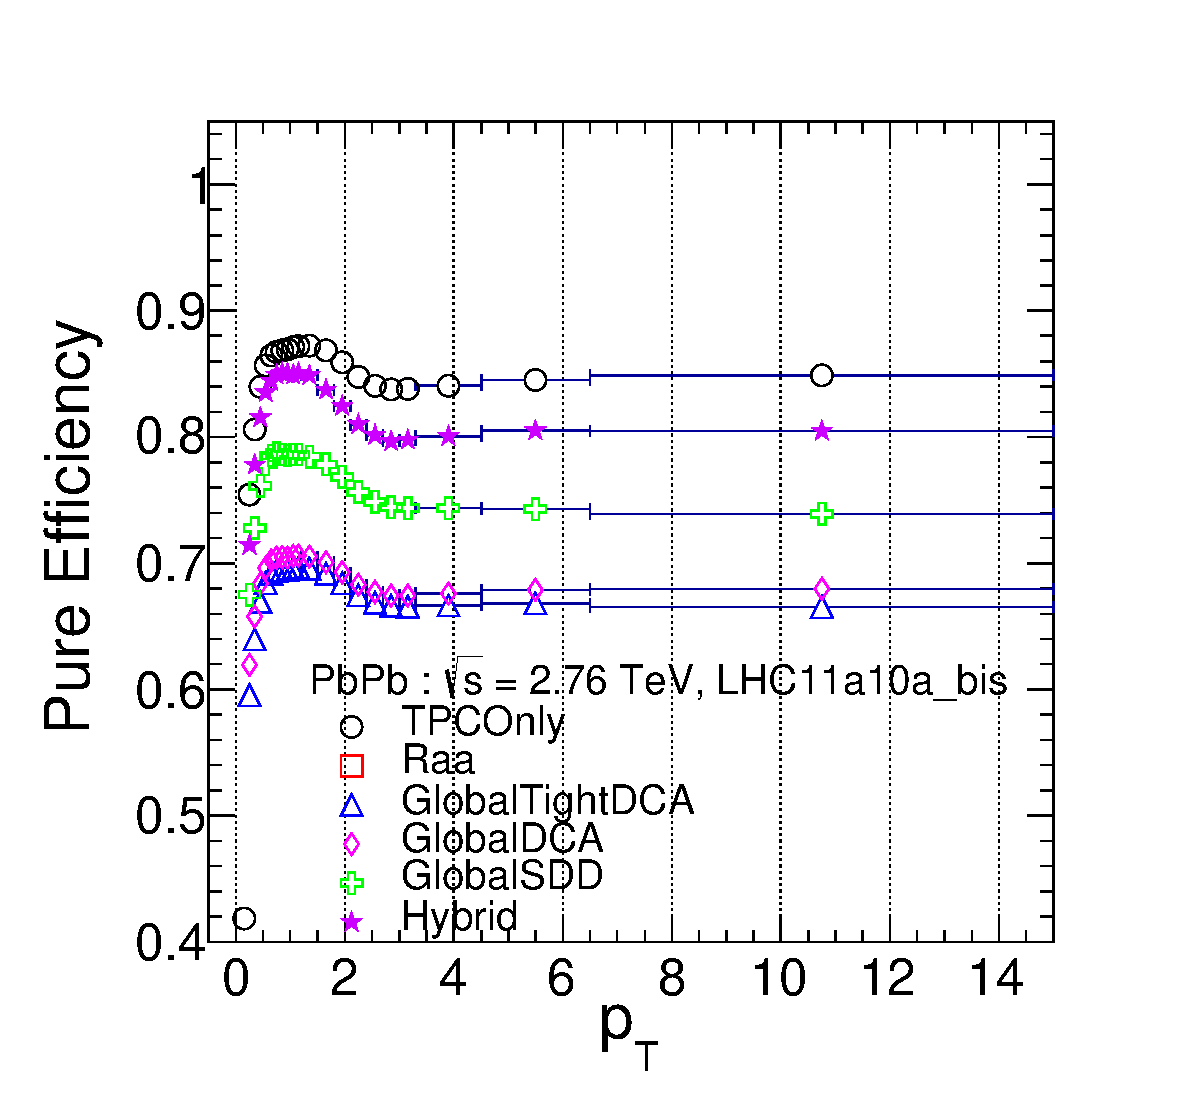
\includegraphics{figures/figs_systematics/PureEfficiency_PbPb276}}
        	\resizebox{0.65\columnwidth}{!}{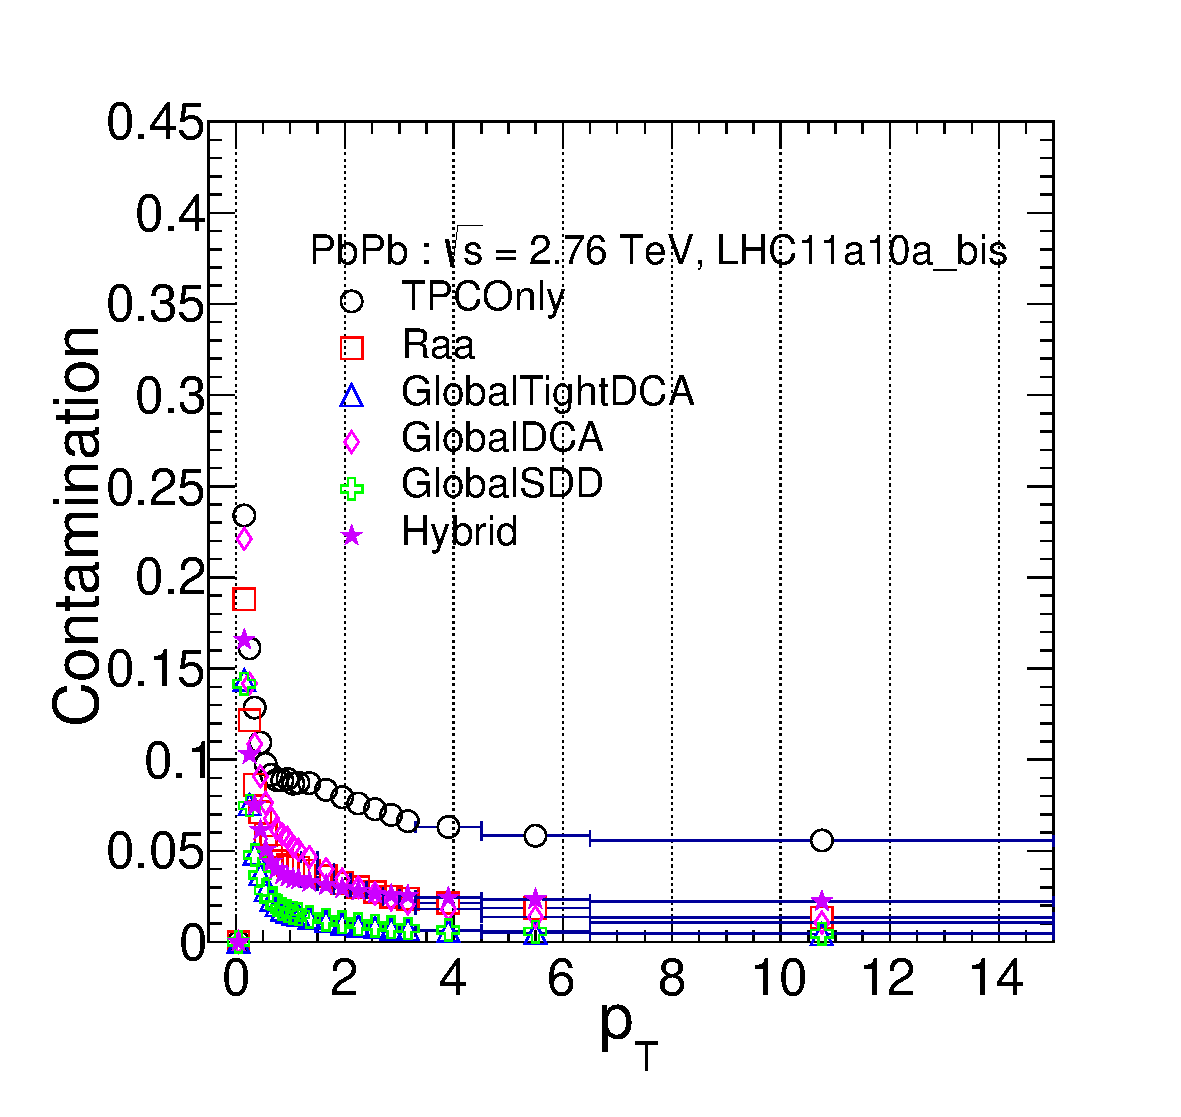
\includegraphics{figures/figs_systematics/Contamination_PbPb276}}
        \caption{Tracking efficiency of single particle reconstruction as a function of $p_T$ (left) and contamination of single particle as a function of $p_T$ (right) for ALICE with various track selection filter}
        \label{fig:eff}
        \end{center}   
     \end{figure}



\subsection{Overall systematic uncertainty}

All systematic uncertainty checks discussed in this analysis were included in the final systematic uncertainty. All individual checks are performed independently and these all systematics were combined in quadrature to obtain the final uncertainty. The tabulated systematic uncertainties are listed below tables.

\begin{table}[!p]
\begin{tabular}{c|c|c|c|c|c}
 
  Type  [\%]						&   SC(3,2)   &  SC(4,2) & SC(5,2) & SC(5,3) & SC(4,3)\\   \hline  \hline
  Non-uniform $\phi$ distribution	& $<1$	& 1.2	&9.5 	&17.3	&11.3	  	\\ \hline
  Track filter bit selection 		& 8.4	& 4.9	&9.1	&9.1		&11.9	 	\\ \hline
  Efficiency correction				& 3.1	& 4.4	&1.5	&1.7		&1.3	 \\ \hline
  Z-vertex cut						& 2.1	& 1.5	&2.1	&1.9		&3.0	\\ \hline
  Charge combination				& 4.5	& 12.1	&18.5	&19.5	&6.8 	\\ \hline
  high multiplicity outliers			& $<1$	& 2		&2.1	&2.1		&$<1$	\\ \hline
  Magnetic field polarization		& 2.1	& 2.7	&1.3	&1.5		&1.1	 \\ \hline   
  Centrality determination			& $<1$	& $<1$	&3.1	&7.6		&1.5 	\\ \hline   \hline
  Overall 							& 10.8	& 17.9	&22.8	&28.8	&18.4
  
\end{tabular}
\caption{Systematic uncertainties of $SC(m,n)$. Overall systematics are quadratically merged results of each individual systematic error}
\end{table}

\begin{table}[!p]
\begin{tabular}{c|c|c|c|c|c}
 
  Type  [\%]						&   NSC(3,2)   &  NSC(4,2) & NSC(5,2) & NSC(5,3) & NSC(4,3)\\   \hline  \hline
  Non-uniform $\phi$ distribution	& $<1$	& 1.1	&7.5 	&15.3	&12.4	  	\\ \hline
  Track filter bit selection 		& 7.3	& 4.9	&8.4	&12.1	&11.1	 	\\ \hline
  Efficiency correction				& 3.1	& 3.4	&1.5	&1.7		&1.3	 \\ \hline
  Z-vertex cut						& 2.1	& 1.5	&2.1	&1.9		&3.0		\\ \hline
  Charge combination				& 2.3	& 5.1	&18.2	&19.5	&6.1 	\\ \hline
  high multiplicity outliers			& $<1$	& 2		&2.1	&3.1		&$<1$	\\ \hline
  Magnetic field polarization		& 2.1	& 2.7	&3.6	&5.1		&4.1	 \\ \hline   
  Centrality determination			& $<1$	& $<1$	&1.4	&1.5		&$<1$ 	\\ \hline   \hline
  Overall 							& 9.1	& 8.1	&22.2	&28.3	&18.5
  
\end{tabular}
\caption{Systematic uncertainties of $NSC(m,n)$. Overall systematics are quadratically merged results of each individual systematic error}
\end{table}



\clearpage
% !TEX root = main_org.tex
\chapter{Results}

\section{$SC(m,n)$ Results}


\subsection{$SC(3,2)$ and $SC(4,2)$}

The centrality dependence of $SC(4,2)$ and $SC(3,2)$ are presented in Fig.\ref{figs:sc}. Positive values of $SC(4,2)$ are observed for all measured centralities. This suggests a positive correlation between the event-by-event fluctuations of $v_2$ and $v_4$. It also indicates that finding $v_2$ larger than average($\langle v_2 \rangle$) in an event enhances the probability of finding $v_4$ larger than average($\langle v_4 \rangle$) in that event. On the other hand, the negative results of $SC(3,2)$ over all measured centralities show the anti-correlation between $v_2$ and $v_3$ flow harmonic magnitudes, which further implies that finding $v_2$ larger than average($v_2 > \langle v_2 \rangle$) enhancing the probability of finding smaller $v_3$ than average($v_3 < \langle v_3 \rangle$).


	
 	\begin{figure}[!p]
		\begin{center}
        	\resizebox{0.85\columnwidth}{!}{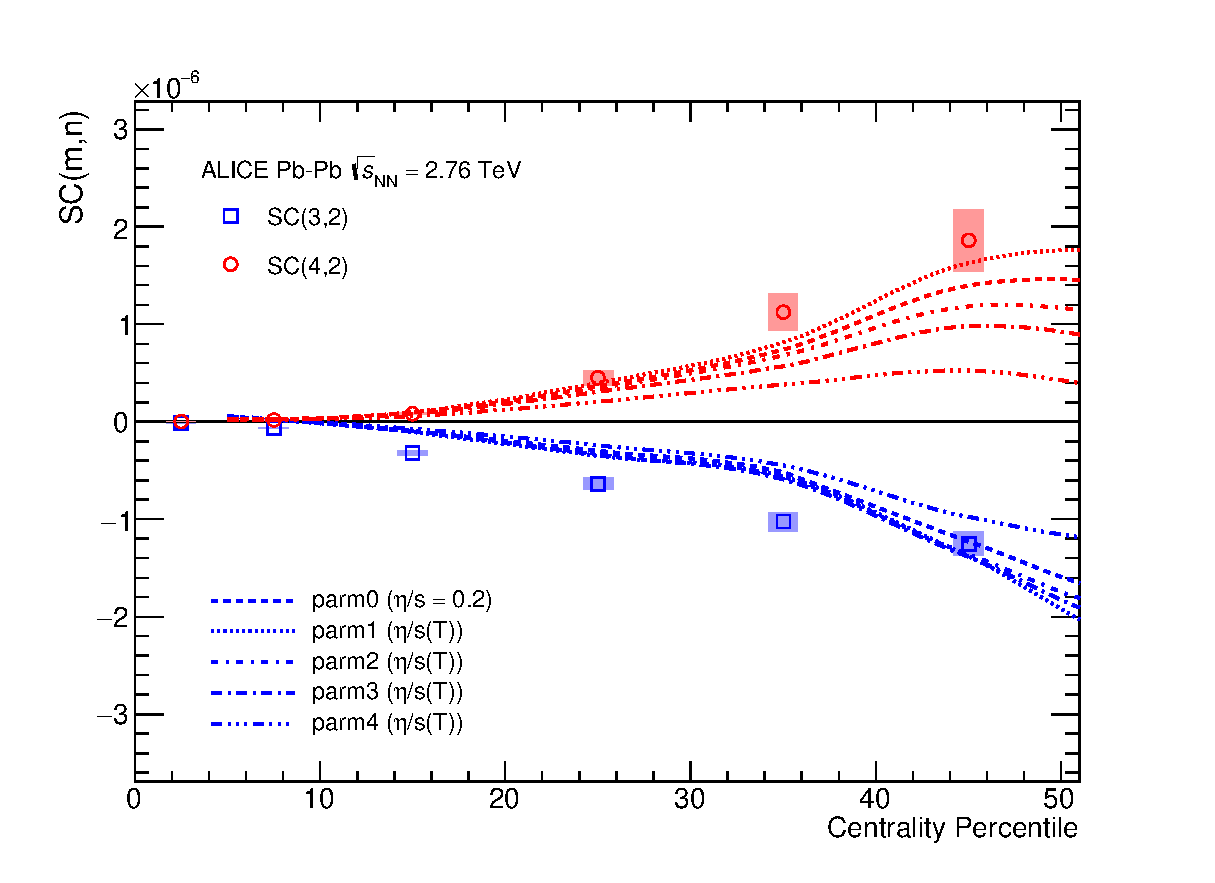
\includegraphics{figures/figs_results/fig1_QConly}}
        	\resizebox{0.85\columnwidth}{!}{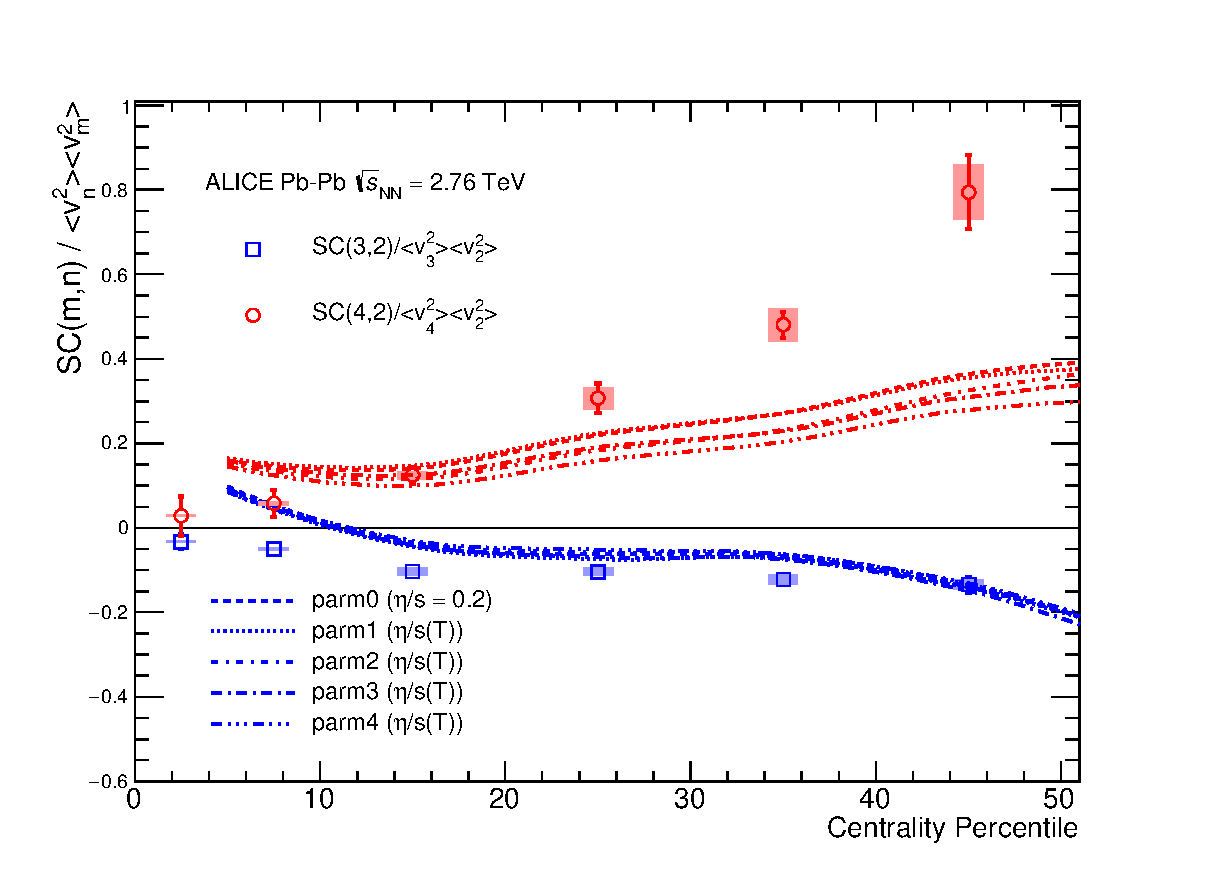
\includegraphics{figures/figs_results/fig1_QConly_norm}}
        \caption{The results of $SC(3,2)$(blue) and $SC(4,2)$(red) with ALICE Pb+Pb $\sqrt{S_{NN}}=2.76$TeV as function of collision centrality (Top). The $NSC(m,n)$ results which scaled with $\langle v_m^2 \rangle \langle v_n^2 \rangle $ were placed in Bottom. The dashed lines are hydrodynamic prediction from H. Niemi with various $\eta / s$ parametrizations \cite{Niemi:2015qia}  }
        \label{figs:sc}
        \end{center}   
     \end{figure}

As discussed and evaluated order-by-order in \cite{Gyulassy:1994ew}, general cumulant formalism is applicable to any correlators eliminating non-flow correlations up to order $2k$ by means of a cumulant expansion. Also when compared with HIJING simulation data\cite{PhysRevD.44.3501} does not include anisotropic collectivity, but has azimuthal correlations due to jet production (non-flow effects)\cite{Borghini:2000sa}.  It is found that both $$\langle \langle \cos{(m\varphi_1 + n\varphi_2 - m\varphi_3 - n\varphi_4)} \rangle \rangle = \langle v_m^2 v_n^2 \rangle $$ and  $$\langle \langle  \cos[m(\varphi_1 - \varphi_2)] \rangle \rangle \langle \langle  \cos[n(\varphi_1 - \varphi_2)] \rangle \rangle = \langle v_m^2 \rangle \langle v_n^2 \rangle$$ are not zero. However, the calculation of $SC(m,n)$ from HJING are compatible with zero for all centralities (even for higher $p_{\rm{T}}$ as shown in Fig.\ref{fig:results_HIJING}) and it suggest that the $SC(m,n)$ are not coming from non-flow effects and insensitive to non-flow correlations.

Moreover, systematics study using the same charge combination pair technique has been done, which is another approach to estimate the non-flow effect. By using like-sign track selection method, we can eliminate ``flow cluster" effects due to charge conservation. As the result of systematic study, it was found that the difference between like-sign and all charged measurements are only few\% level and also we can found same trends (positive and negative correlation for $SC(4,2)$ and $SC(3,2)$) in like-sign results. This further illustrates that non-zero values of $SC(m,n)$ cannot be explained by non-flow effect, but confirms the existence of correlation (and anti-correlations) between $v_n$ and $v_m$ harmonics.

The $SC(m,n)$ results show that the correlation strength in both $SC(m,n)$ and $NSC(m,n)$ increase non-linearly up to centrality 50\%. 

	\begin{figure}[h]
		\begin{center}
        	\resizebox{0.45\columnwidth}{!}{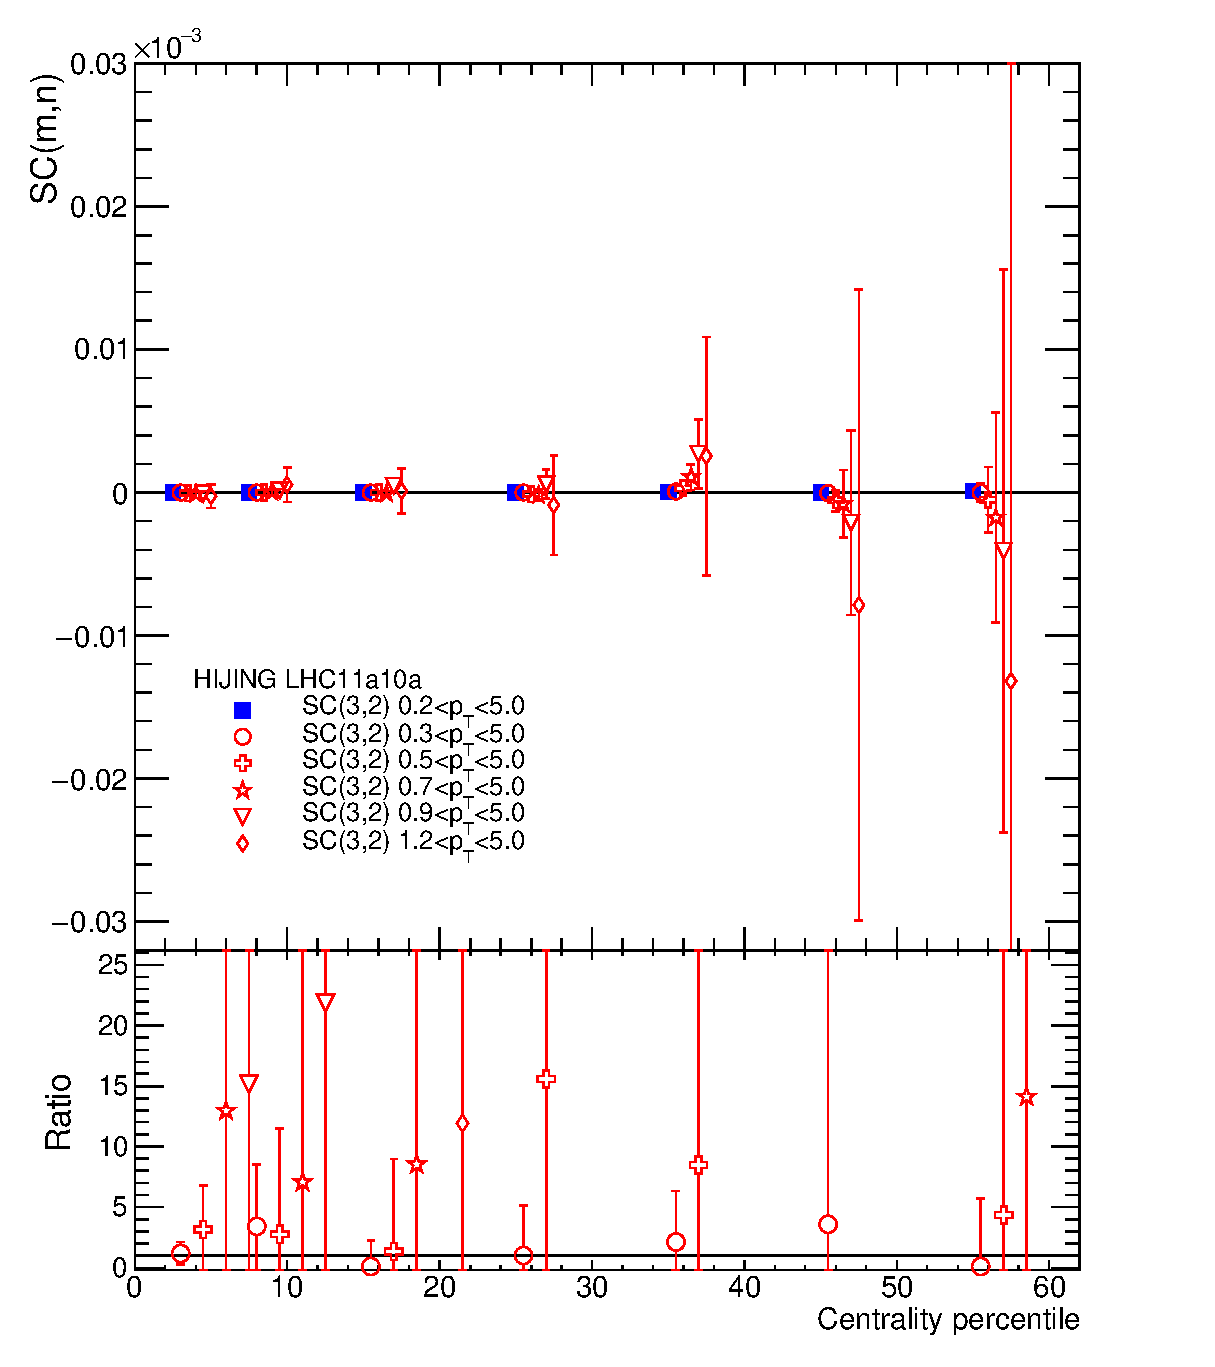
\includegraphics{figures/figs_results/SC_Comparison_SC32_HIJING_ptdep}}
        	\resizebox{0.45\columnwidth}{!}{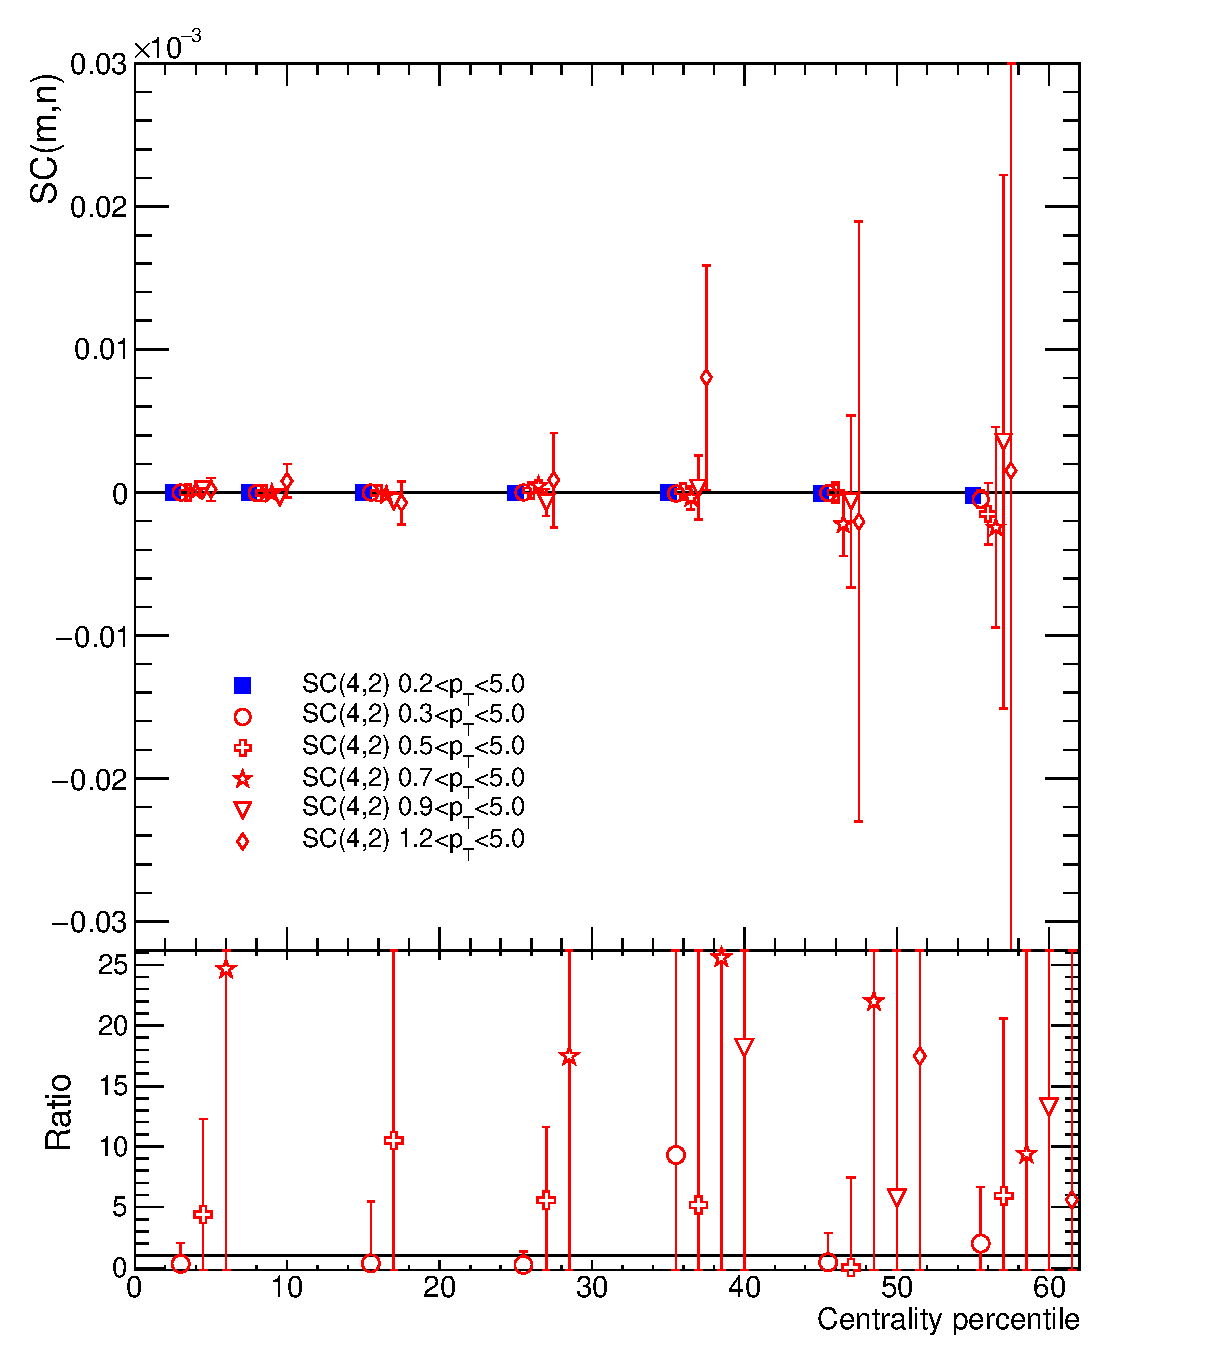
\includegraphics{figures/figs_results/SC_Comparison_SC42_HIJING_ptdep}}
        \caption{The result of SC(3,2) and SC(4,2) with HIJING simulations. Defaults($0.2 < p_{\rm{T}} < 5.0GeV/c$) are drawn as full square with blue color, and different minimum cut conditions are listed in legend. A small shifts along the x axis were applied for better visibility}
        \label{fig:results_HIJING}
        \end{center}   
     \end{figure}



 \subsection{Model Comparison}

Various models have been used in this study. The {HIJING} model~\cite{Wang:1991hta,Gyulassy:1994ew} was used to estimate the strength of non-flow correlations (typically few-particle correlations insensitive to the collision geometry) as described in previous section. 

The $SC(m,n)$ from hydrodynamic prediction with pQCD, where the initial energy density profiles are calculated using a next-to-leading order perturbative-QCD+saturation model~\cite{Paatelainen:2012at,Paatelainen:2013eea} + various shared viscosity $\eta/s$ parameterizations were performed by H. Niemi \cite{Niemi:2015qia}. The subsequent spacetime evolution is described by relativistic dissipative fluid dynamics with different parametrizations for the temperature dependence of the shear viscosity to entropy density ratio $\eta/s(T)$. Each of the $\eta/s(T)$ parametrizations is adjusted to reproduce the measured $v_n$ from central to mid-peripheral collisions. 

 The fluid hydrodynamic predictions with the different parameterizations for the temperature dependence of the shear viscosity to entropy ratio $\eta/s(T)$ are shown shown in Figure.\ref{figs:sc} as dashed line. Roughly the hydrodynamic calculations capture qualitatively the centrality dependence, but not quantitively. Both $SC(3,2)$ with data and hydrodynamics have negative values for all centralities, while $SC(4,2)$ results have positive values over all measured centralities. However, there is no single centrality for which a given $\eta/s(T)$ parameterization describes both $SC(3,2)$ and $SC(4,2)$ simultaneously. On the other hand, the same hydrodynamic calculations capture the centrality dependence of the individual $v_n$ quantitively~\cite{Eskola:2015uda}.

$NSC(3,2)$ and $NSC(4,2)$ are also compared to the same model on the right in Fig.~\ref{figs:sc}. 
While $NSC(3,2)$ does not show sensitivity to  different $\eta/s(T)$ parameterizations,  $NSC(4,2)$ exhibit much better sensitivity
than $NSC(3,2)$ observable and the individual flow harmonics~\cite{Niemi:2015qia}.
These findings indicate that $NSC(3,2)$ observable is sensitive mainly to the initial conditions, while $NSC(4,2)$ observable is sensitive to both the initial conditions and the system properties, which is consistent with the prediction from~\cite{Niemi:2012aj}.

However, the sign of $NSC(3,2)$ is positive in the models in 0-10\% central collisions while it is negative in data.
In the most central collisions the anisotropies originate mainly from fluctuations, i.e.\ the initial ellipsoidal geometry characteristic for mid-central collisions plays little role in this regime. Hence this observation will help to understand the fluctuations in initial conditions better.

$NSC(4,2)$ observable shows better sensitivity for different $\eta/s(T)$ parameterizations, i.e. medium property but the model cannot describe the centrality dependence nor the absolute values. These observed distinct discrepancies between data and models might indicate that the current understanding of initial conditions used in the model need to be revisited
to further constrain the $\eta/s(T)$, considering the difficulties on separating the role of the $\eta/s$  from the initial condition to the final state particle anisotropies~\cite{Romatschke:2007mq,Shen:2011zc}.
Hence the use of $SC(m,n)$ and $NSC(m,n)$ can provide new constraints on the detailed modeling of the initial-state condition and the fluctuations of the medium created in heavy ion collisions and the better constraints on the initial-state conditions will certainly improve the uncertainties of determining $\eta/s(T)$.



 The  $NSC(m,n)$ were compared to MC-Glauber using wounded nucleon (WN) and binary collisions (BC) weights models to check linear and non-linear response from initial geometry.  Assuming only linear response $v_n \propto \epsilon_n$, we expect that the normalized $SC(m,n)$ evaluated in coordinate space are able to capture the measurement of centrality dependence of normalized $SC(m,n)$ in the momentum space. In this case the correlation between the $n$th and $m$th order harmonics were estimated with calculation of $SC(m,n)$ in the coordinate space as define as 
 
 \begin{equation}
SC(m,n)_{\epsilon}/\langle \epsilon_n^2 \rangle \langle \epsilon_m^2 \rangle  \equiv (\langle \epsilon_n^2 \epsilon_m^2 \rangle - \langle \epsilon_n^2 \rangle \langle \epsilon_m^2 \rangle) /  \langle \epsilon_n^2 \rangle \langle \epsilon_m^2 \rangle
\label{eq:sc_ecen}
\end{equation}

Where the $\epsilon_n$ is the $n$th order coordinate space anisotropy as defined in \cite{Alver:2010gr}. Since there are two different scenarios of the MC-Glauber model, we tested with both wounded nucleon (WN) and binary collisions (BC) weights and results are shown in Fig.\ref{fig:results_ecen}. An increasing trend from central to peripheral collisions with different sign has been observed and there is a large deviation of $NSC(4,2)$ between ALICE data and MC-Glauber model. This deviation increase from central to peripheral collision regions and this might indicate the contribution of the non-linear response of initial condition though hydrodynamic evolution. Moreover, the MC-Glauber model with  $NSC(3,2)$ describes better the data  than $NSC(4,2)$,  because the  $NSC(3,2)$ appears to be sensitive only to initial conditions and not sensitive to hydrodynamic properties ($\eta/s$). 


	\begin{figure}[h]
		\begin{center}
        	\resizebox{0.45\columnwidth}{!}{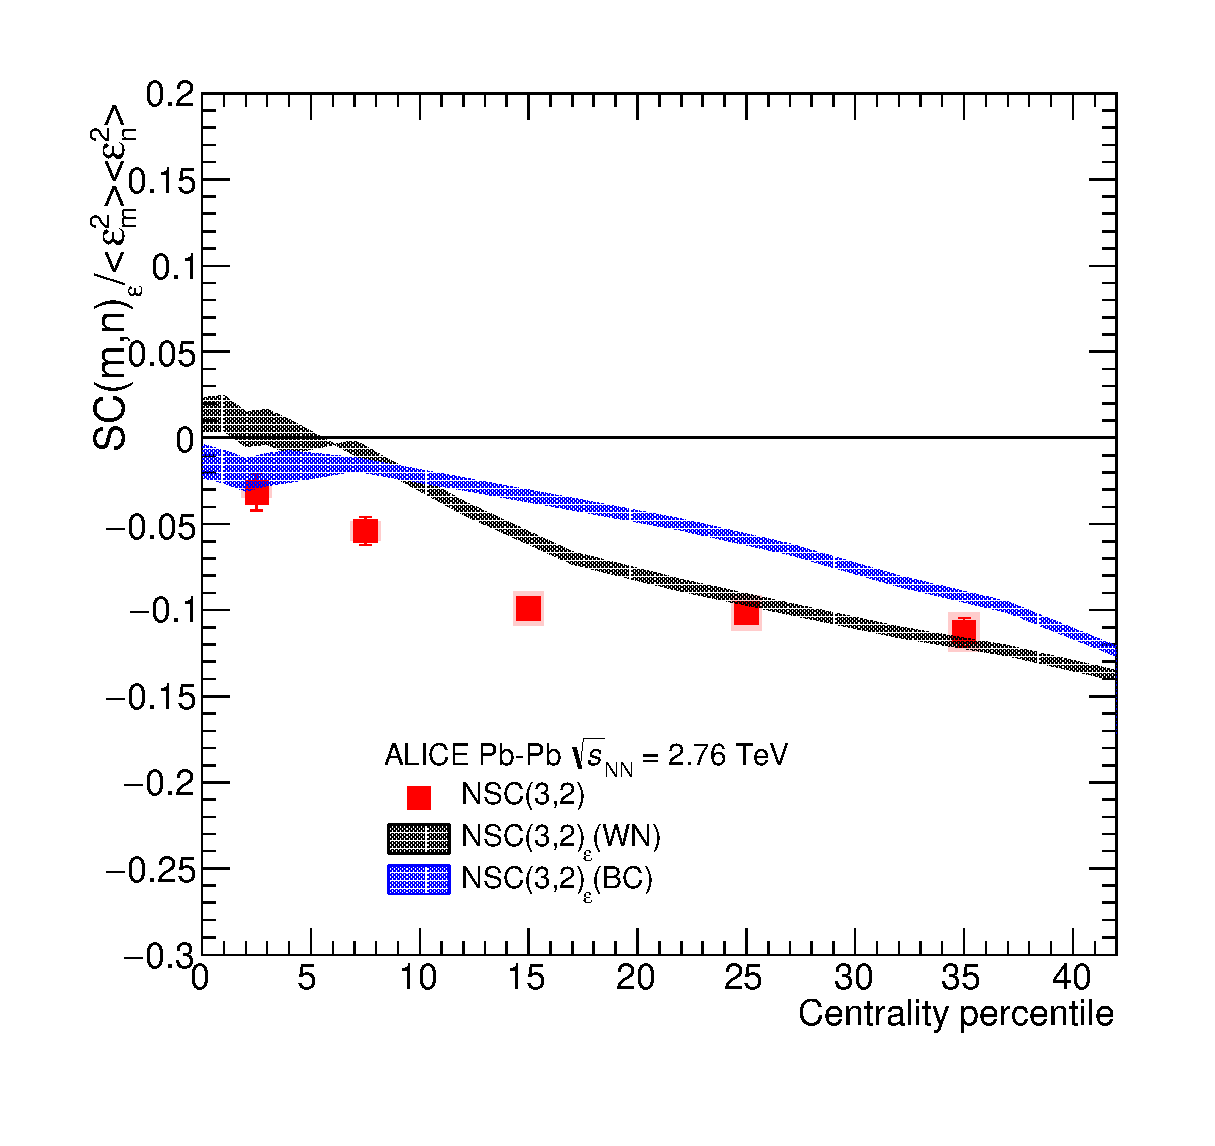
\includegraphics{figures/fig_ecen/SC_Comparison_ecen_BC_SC32}}
        	\resizebox{0.45\columnwidth}{!}{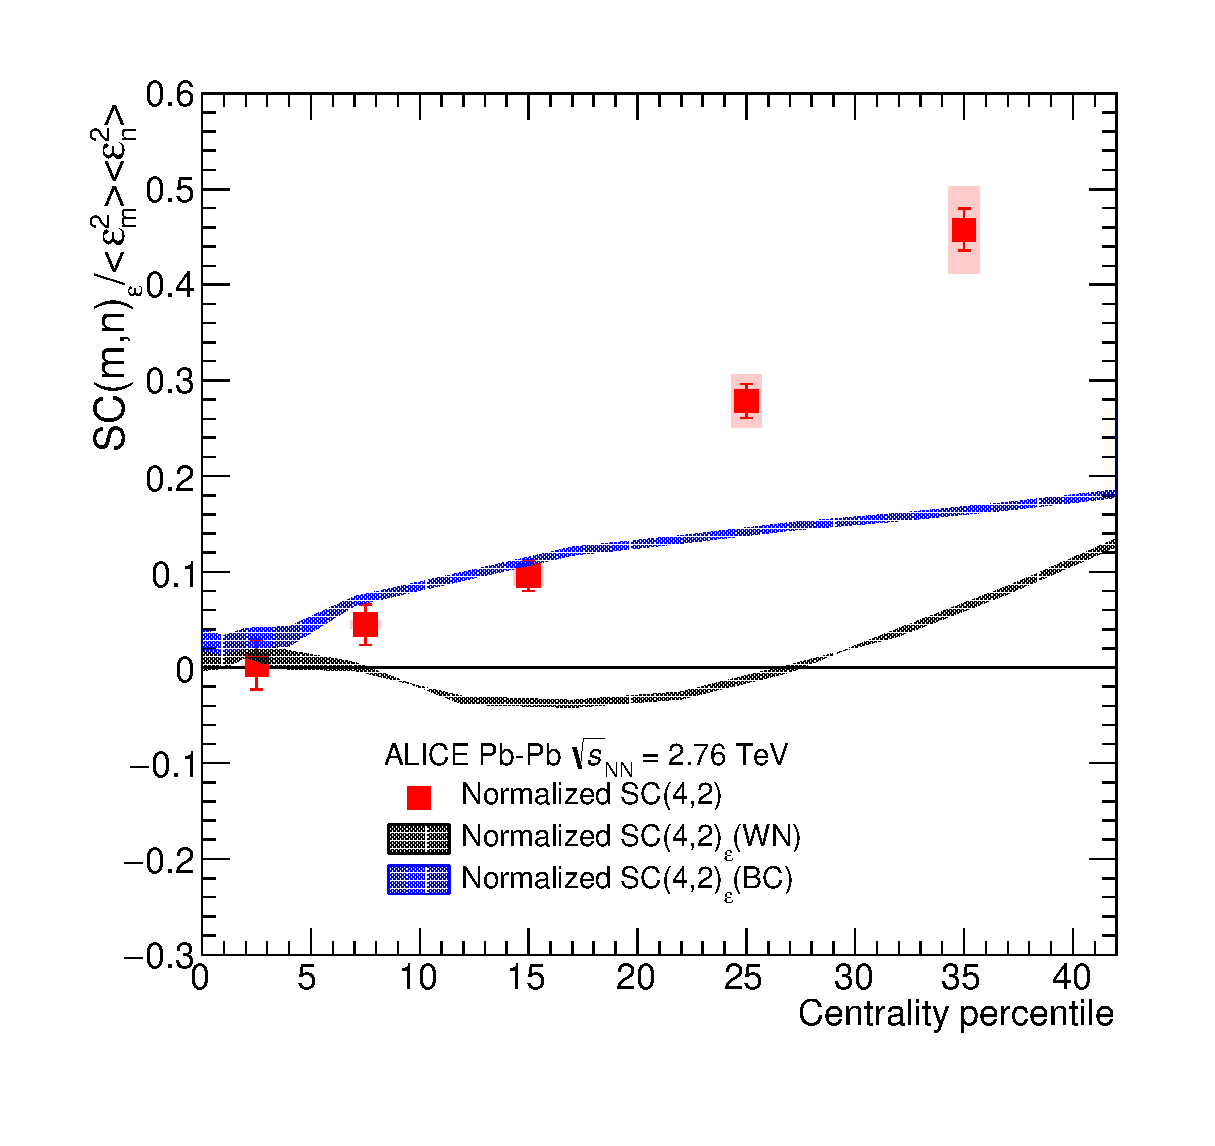
\includegraphics{figures/fig_ecen/SC_Comparison_ecen_BC_SC42}}
        \caption{$NSC(m,n)$(red) and $NSC(m,n)_\epsilon$ (correlation in coordinate space) by using MC-Glauber models with wounded nucleon (WN) and binary collisions (BC) weights.}
        \label{fig:results_ecen}
        \end{center}   
     \end{figure}



 $SC(m,n)$ with AMPT \cite{Zhang:1999bd,Lin:2000cx,Lin:2004en} simulation with various configurations was also tested. The configuration of AMPT are listed in Table.\ref{Tab:AMPTConf}. With changing configuration of AMPT simulations, we may estimate the effects of initial conditions and finite states effects. 

Even though thermalization could be achieved in collisions of very large nuclei and/or at extremely high energy, the dense matter created in heavy ion collisions may not achieve full thermal or chemical equilibrium as a result of its finite volume and energy. To address such non-equilibrium many-body dynamics, AMPT has been developed, which includes both initial partonic and final hadronic interactions and the transition between these two phases of matter.
For the initial conditions, the AMPT model uses the spatial and momentum distributions of hard minijet partons and soft strings from the HIJING model~\cite{Wang:1991hta,Gyulassy:1994ew}.
The AMPT model can be run in two main configurations, the default and the string melting model.
In the default version, partons are recombined with their parent strings when they stop interacting. The resulting strings are later converted into hadrons using the Lund string fragmentation model~\cite{Andersson:1986gw,NilssonAlmqvist:1986rx}. In the string melting version,  all the excited strings that are not projectile and target nucleons not experiencing any interactions are converted to partons according to the flavor and spin structures of their valence quarks. The advantage of this choice is that the AMPT model with string melting reduces to HIJING results in the absence of partonic and hadronic interactions as these partons would then find each other as closest partners at the same freeze-out time and thus coalesce back to the original hadron. In the AMPT model with string melting, the initial strings are melted into partons whose interactions are described by the ZPC parton cascade model~\cite{Zhang:1997ej}. These partons are then combined into the final-state hadrons via a quark coalescence model.  \cite{Lin:2005br}

In both configurations, the dynamics of the subsequent hadronic matter is described by a hadronic cascade based on a Relativistic Transport (ART) model~\cite{Li:2001xh} which also includes resonance decays.
The third version presented in this article is based on the string melting configuration, in which the hadronic rescattering phase is switched off to study its influence to the development of anisotropic flow.
The input parameters used in both configurations are: $\alpha_s = 0.33$, a partonic cross-section of 1.5~mb, while the Lund string fragmentation parameters were set to $\alpha = 0.5$ and $b = 0.9$~GeV$^{-2}$. 
Even though the string melting version of AMPT~\cite{Lin:2001zk,Lin:2004en} reasonably reproduces particle yields, $p_{\rm{T}}$ spectra, and $v_2$ of low-$p_{\rm{T}}$ pions and kaons in central and mid-central Au-Au collisions at $200$~GeV and Pb-Pb collisions at $2.76$~TeV~\cite{Lin:2014tya}, it was seen clearly in the recent study~\cite{Adam:2016nfo} that it fails to quantitatively reproduce the measurements. It turns out that the radial flow in AMPT is 25\% lower than the measured value at the LHC, which indicates that the unrealistically low radial flow in AMPT is responsible for the quantitative disagreement. The detail configurations on AMPT settings used for this article and the comparisons of $p_{\rm{T}}$ differential $v_{n}$ for pions, kaons and protons to the data can be found in \cite{Adam:2016nfo}.






\begin{table}[!h]
\begin{center}
\begin{tabular}{c|c|c}
\hline 
Setting		    & String Melting    & Rescattering  \\  \hline  \hline
AMPT Default  & OFF     & ON        \\ \hline
AMPT String melting  & ON      &  ON        \\ \hline 
AMPT String melting w/o hadronic rescattering  & ON      & OFF         \\ \hline
\label{Tab:AMPTConf}
\end{tabular}
\caption{Configurations of AMPT simulation dataset which correspond to ALICE LHC10h data with Pb+Pb $\sqrt{S_{NN}}=2.76$TeV}
\end{center}
\end{table}


	\begin{figure}[!p]
		\begin{center}
        	\resizebox{0.48\columnwidth}{!}{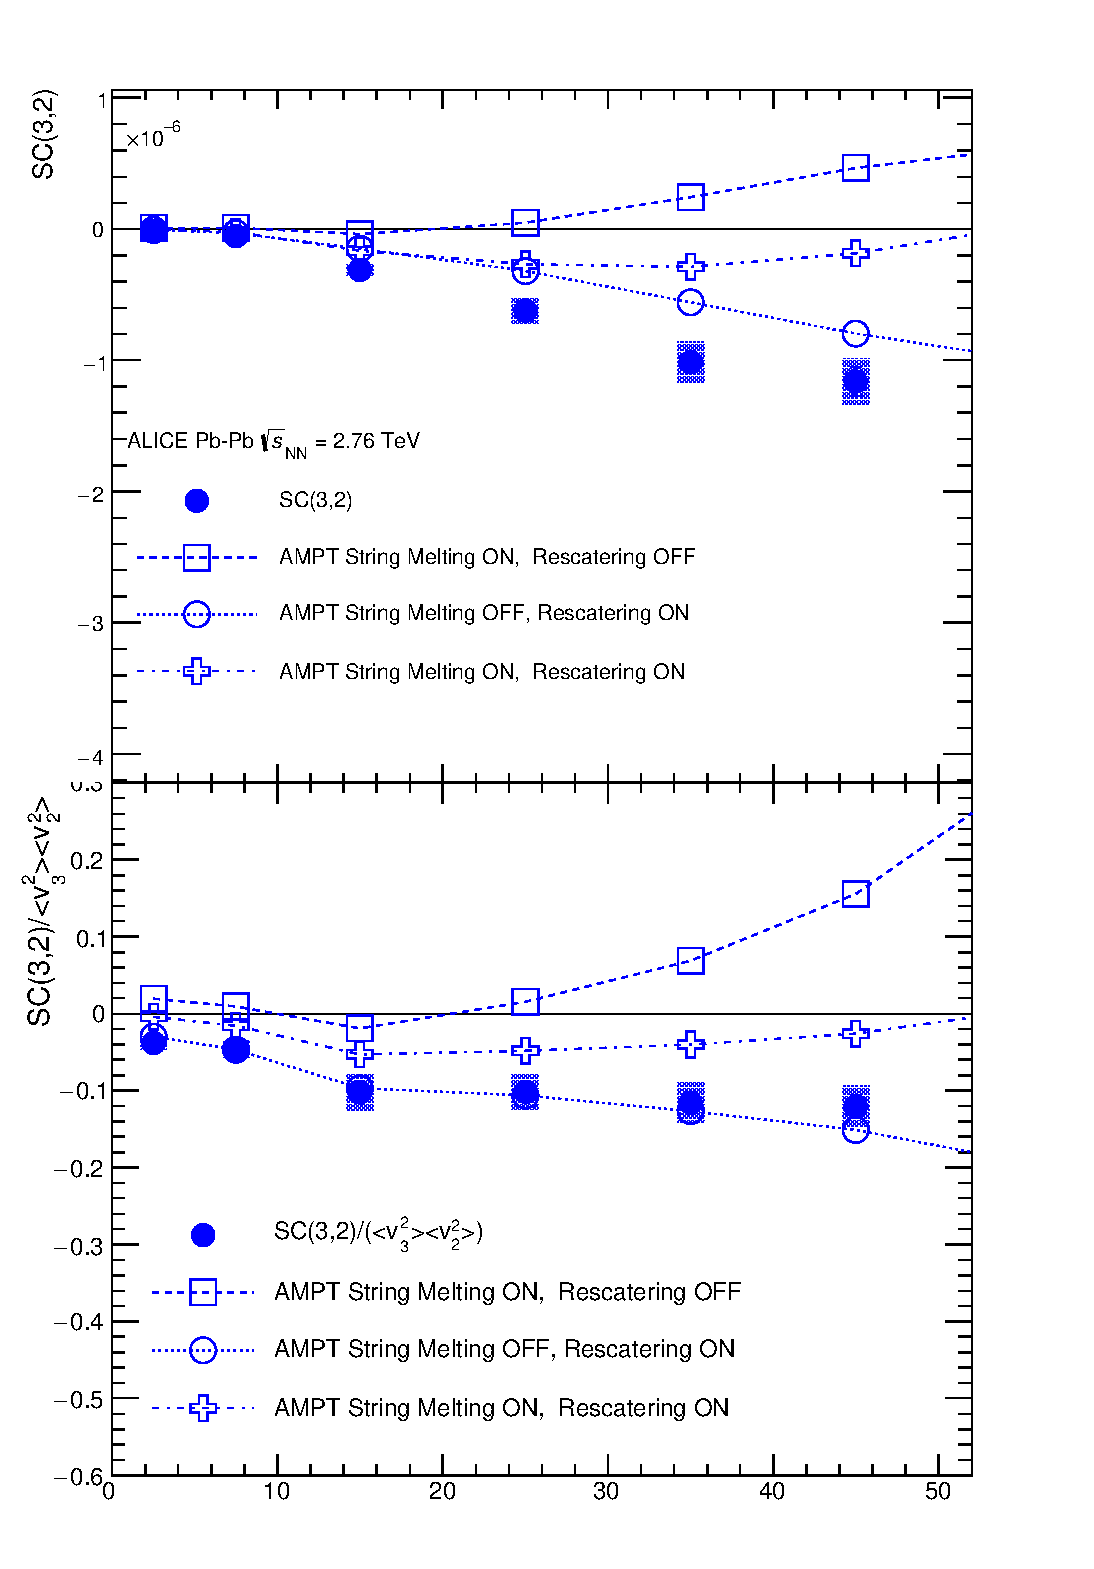
\includegraphics{figures/figs_results/fig3_QConly_ModelComparison_SC32_ampt.eps}}
        	\resizebox{0.48\columnwidth}{!}{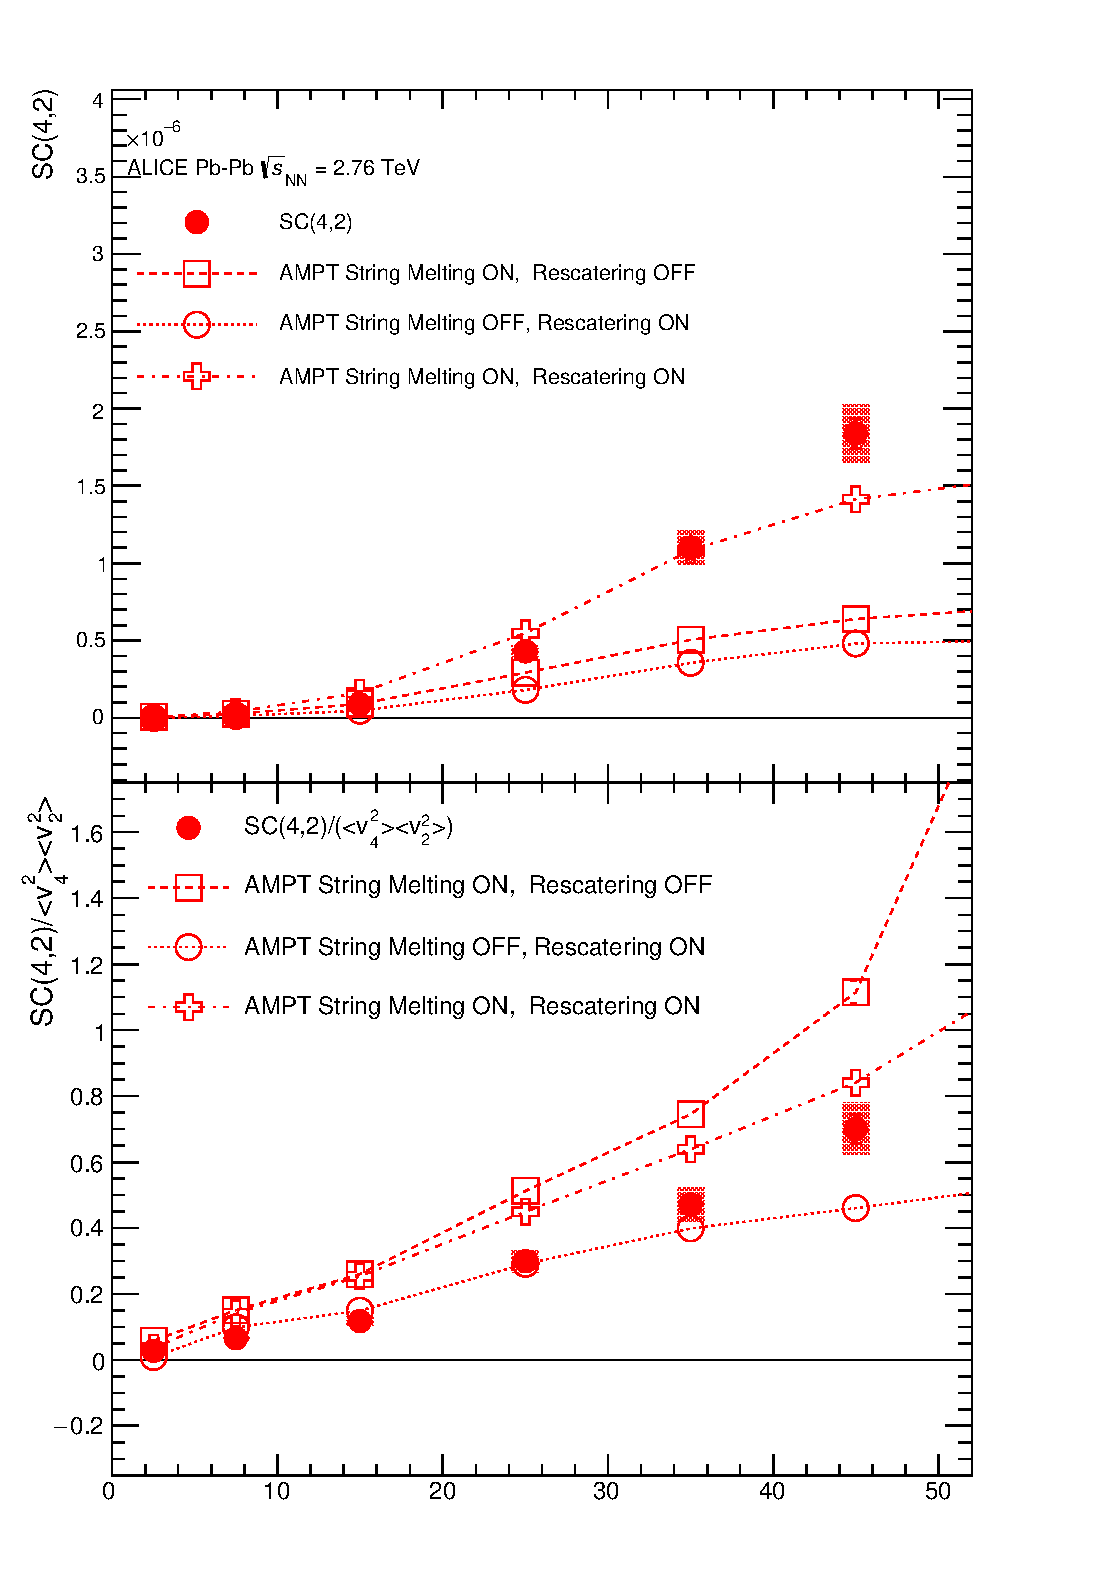
\includegraphics{figures/figs_results/fig3_QConly_ModelComparison_SC42_ampt.eps}}
        \caption{The result of  $SC(3,2)$ and $SC(4,2)$ with ALICE data and comparison to various AMPT simulations with different settings.  The upper figures are the results of $SC(m,n)$ and the lower figures are the results of normalized $SC(m,n)$}
        \label{AMPTcomLowSC}
        \end{center}   
     \end{figure}

The results of comparison to AMPT are shown in Fig.\ref{AMPTcomLowSC}. As for $SC(3,2)$, neither of the settings can describe the data and somewhat the setting with the default AMPT model follows the trend of the data closest. The same setting can describe NSC(3,2) fairly well and also the sign of NSC(3,2) is well reproduced by this setting while all the hydrodynamic calculations in this article failed to describe the sign of the observable in most central collisions.

Interestingly the string melting AMPT model can't capture the data well where the strength of the correlation is weaker than the default model. The third version based on the string melting configuration with the hadronic rescattering phase off is also shown to study its influence. This late hadronic rescattering stage makes both $SC(3,2)$ and $NSC(3,2)$ stronger in the string melting AMPT model but it is not enough to describe the data.

Further we investigated why the default AMPT model can describe $NSC(3,2)$ fairly well but underestimates $SC(3,2)$. By taking the differences in the individual flow harmonics ($v_2$ and $v_2$) between the model and data into account, we was able to recover the data. The discrepancy in $SC(3,2)$ can be explained by the overestimated individual $v_n$ values reported in \cite{Adam:2016nfo} in all the centrality ranges. 

In case of $SC(4,2)$, the string melting AMPT model can fairly describe the data while the default model underestimates it.
$NSC(4,2)$ is slightly overestimated by the same setting which can describe $SC(4,2)$ but the default AMPT model can describe the data better.
The influence of the hadronic rescattering phase for $NSC(4,2)$ is opposite to other observables ($SC(3,2)$, $NSC(3,2)$ and $SC(4,2)$), where the hadronic rescattering make $NSC(4,2)$ slightly smaller.
It should be noted that the better agreement for $SC(m,n)$ should not be overemphasized since there are discrepancies in the individual $v_n$ between AMPT and data as it was demonstrated for $SC(3,2)$.
Hence the simultaneous description of $SC(m,n)$ and $NSC(m,n)$ should give better constrains to the parameters in AMPT.



	\begin{figure}[!p]
		\begin{center}
        	\resizebox{0.48\columnwidth}{!}{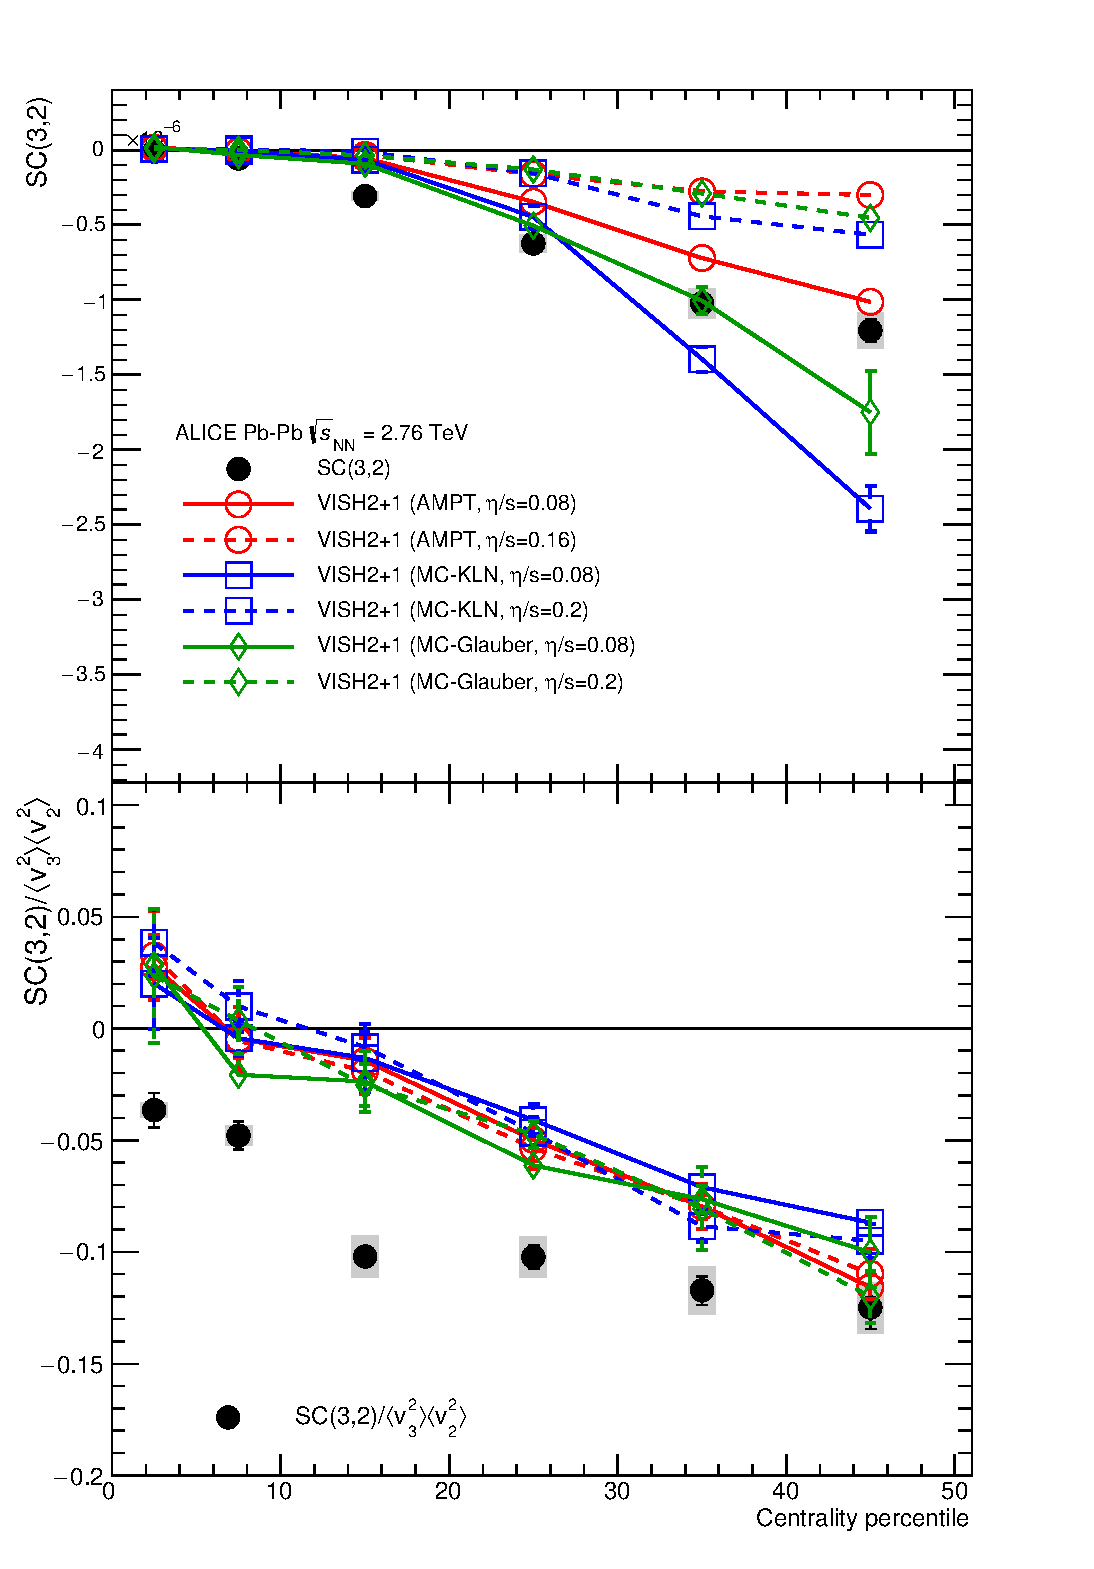
\includegraphics{figures/figs_results/fig3_QConly_ModelComparison_SC32_vish.eps}}
        	\resizebox{0.48\columnwidth}{!}{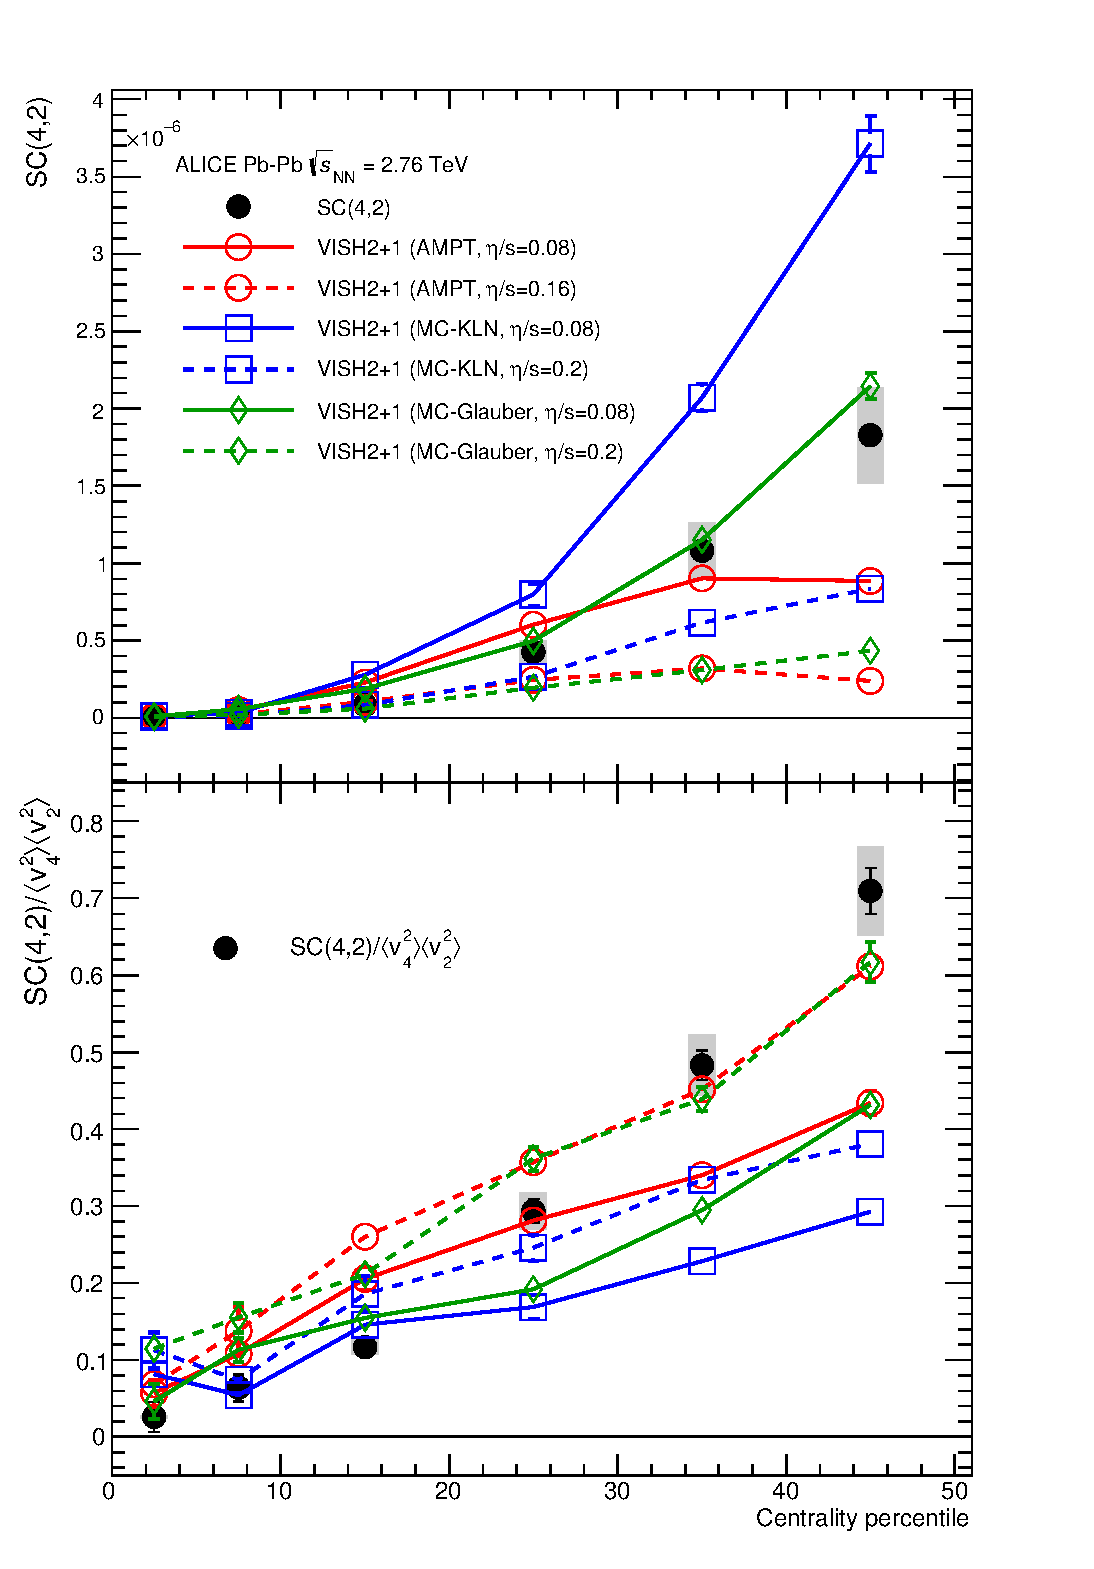
\includegraphics{figures/figs_results/fig3_QConly_ModelComparison_SC42_vish.eps}}
        \caption{Result of  $SC(3,2)$(left) and $SC(4,2)$(right) with LHC10h data and various VISH2+1 calculation with different settings. The three initial conditions from AMPT, KLN, and Glauber simulations are drawn as a different color. Furthermore, the hydrodynamic properties of $\eta/s$ are shown as line style, the small share viscosity ($\eta/s$=0.08) are shown as solid line, and large share viscosity ($\eta/s$=0.2 for KLN and Glauber, 0.16 for AMPT) is drawn as dashed line. Upper figures are the result of $SC(m,n)$ and lower figures are results of normalized $SC(m,n)$}
        \label{vish21}
        \end{center}   
     \end{figure}


  The comparison to VISH2+1 calculation are shown in Fig.\ref{vish21}. The VISH2+1~\cite{Zhu:2016puf} is an event-by-event theoretical framework model for relativistic heavy-ion collision based on (2+1)-dimensional viscous hydrodynamics which describes both the QGP fluid and the highly dissipative and even off-equilibrium late hadronic stage with fluid-dynamics. With well tuned transport coefficients, decoupling temperature  and some well-chosen initial conditions (like {AMPT}~\cite{Xu:2016hmp,Bhalerao:2015iya,Pang:2012he} etc.), it could fit many related soft hadron data, such as the $p_{\rm{T}}$ spectra and different flow harmonics at RHIC and the LHC~\cite{Qiu:2011hf, Shen:2010uy, Shen:2011eg, Bhalerao:2015iya}.
Three different initial conditions ({MC-Glauber}, {MC-KLN} and {AMPT}) along with different constant $\eta/s$ parametrizations are used in the model. 
Traditionally, the Glauber model constructs the initial entropy density of the QGP fireball from a mixture of the wounded nucleon and binary collision density profiles~\cite{Kolb:2000sd}, and the {KLN} model assumes the initial entropy density is proportional to the initial gluon density calculated from the corresponding $k_T$ factorization formula~\cite{Kharzeev:2000ph}. In the Monte-Carlo versions ({MC-Glauber} and {MC-KLN})~\cite{Miller:2007ri,Drescher:2006ca,Hirano:2009ah}, additional initial state fluctuations are introduced through the position fluctuations of individual nucleons inside the colliding nuclei. For the {AMPT} initial conditions~\cite{Bhalerao:2015iya,Pang:2012he,Xu:2016hmp}, the fluctuating energy density profiles are constructed from the energy decompositions of individual partons, which fluctuate in both momentum and position space. Compared with the {MC-Glauber} and {MC-KLN} initial conditions, the additional Gaussian smearing parameter in the {AMPT} initial conditions makes the typical initial fluctuation scales changeable which gives rise to non-vanishing initial local flow velocities~\cite{Pang:2012he}. 

As shown in the Fig.\ref{vish21},  all the models with the large share viscosity regardless of the initial conditions ($\eta/s$=0.2 for MC-KLN and MC-Glauber initial conditions and $\eta/s = 0.16$ for AMPT initial condition) failed to capture the centrality dependence of $SC(3,2)$ and $SC(4,2)$.  However, for the normalized case($NSC$), all the results with different parameters do not have much difference as like original $SC(m,n)$. It may suggest that the $\eta/s$ parametrization affects the single flow magnitude, (generally large share viscosity($\eta/s$) leads short mean free path($\lambda_{mfp}$) and it decreases the flow magnitudes) rather than affect on correlations between flow orders. 
And among the models with small shear viscosities ($\eta/s$=0.08), the one with the AMPT initial condition describes the data better both for $SC(3,2)$ and $SC(4,2)$ but they cannot describe the data quantitively for most of the centrality ranges.
As similarly as the above mentioned hydrodynamic calculations~\cite{Niemi:2015qia}, the sign of the $NSC(3,2)$ in these models is opposite to the data in 0-10\% central collisions. $NSC(3,2)$ don't show sensitivity to neither initial conditions nor $\eta/s$ parameterizations and cannot be described by these models quantitively.
However, for $NSC(4,2)$, it is sensitive both to initial conditions and $\eta/s$ parameterizations.
Even though $NSC(4,2)$ is favored both by AMPT initial condition with $\eta/s$=0.08 and MC-Glauber initial condition with $\eta/s$=0.20,
$SC(4,2)$ can be only described by smaller $\eta/s$ from AMPT and MC-Glauber initial conditions. Therefore the Glauber initial condition with $\eta/s$=0.20 model can be ruled out and we come to a conclusion based on the tested model parameters that $\eta/s$ should be small and AMPT initial condition is favored by the data.
  

\section{Higher order flow harmonics results}

In this section, we will present the results of the correlation between higher order flow harmonics up to 5th order. The results with q-Cumulants method (SP method) with $|\eta| < 0.8$, $0.2 < p_{\rm{T}} < 5.0$GeV/$c$ from ALICE data are shown. The lower order $SC(m,n)$ are scaled down and drawn together as colored band for comparison.


	\begin{figure}[hp]
		\begin{center}
        	\resizebox{0.87\columnwidth}{!}{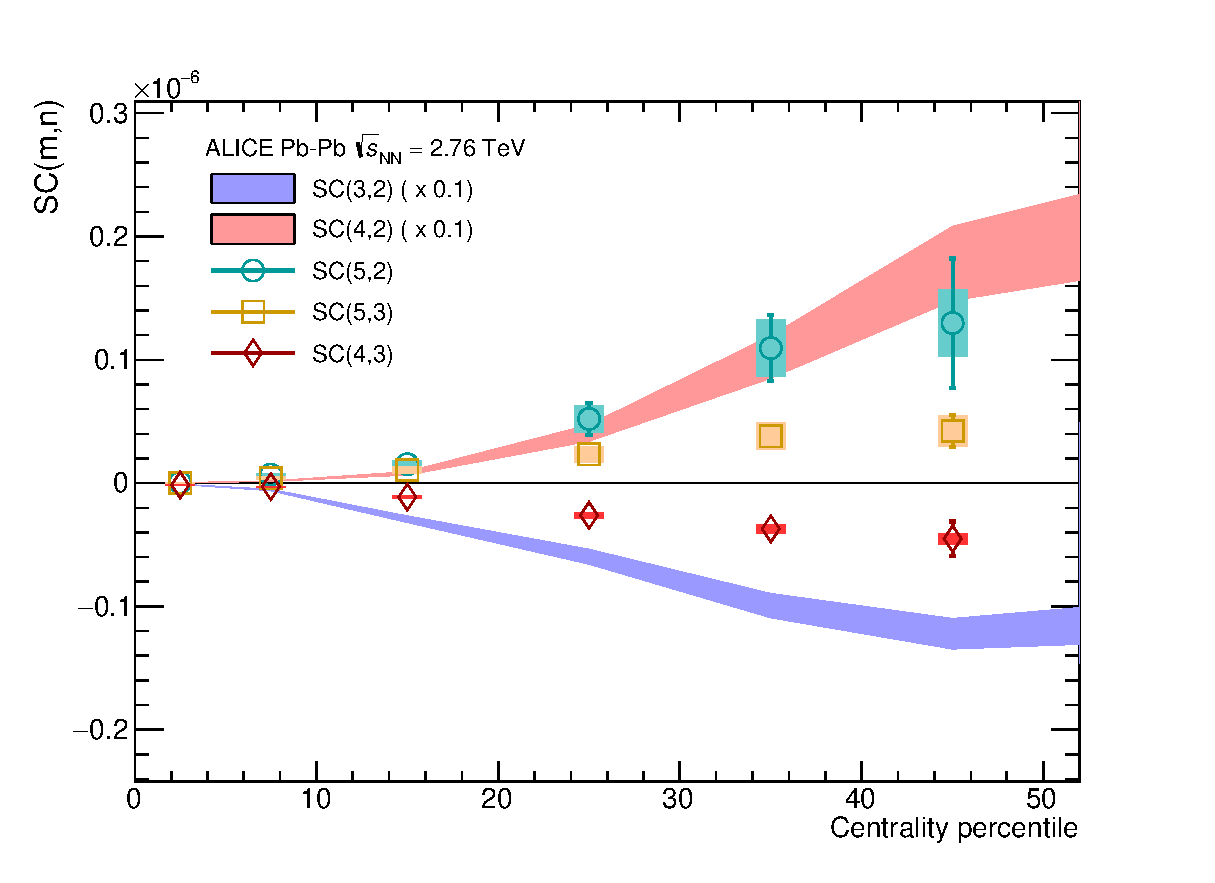
\includegraphics{figures/figs_results/fig2_QConly_higherSC}}
        	\resizebox{0.87\columnwidth}{!}{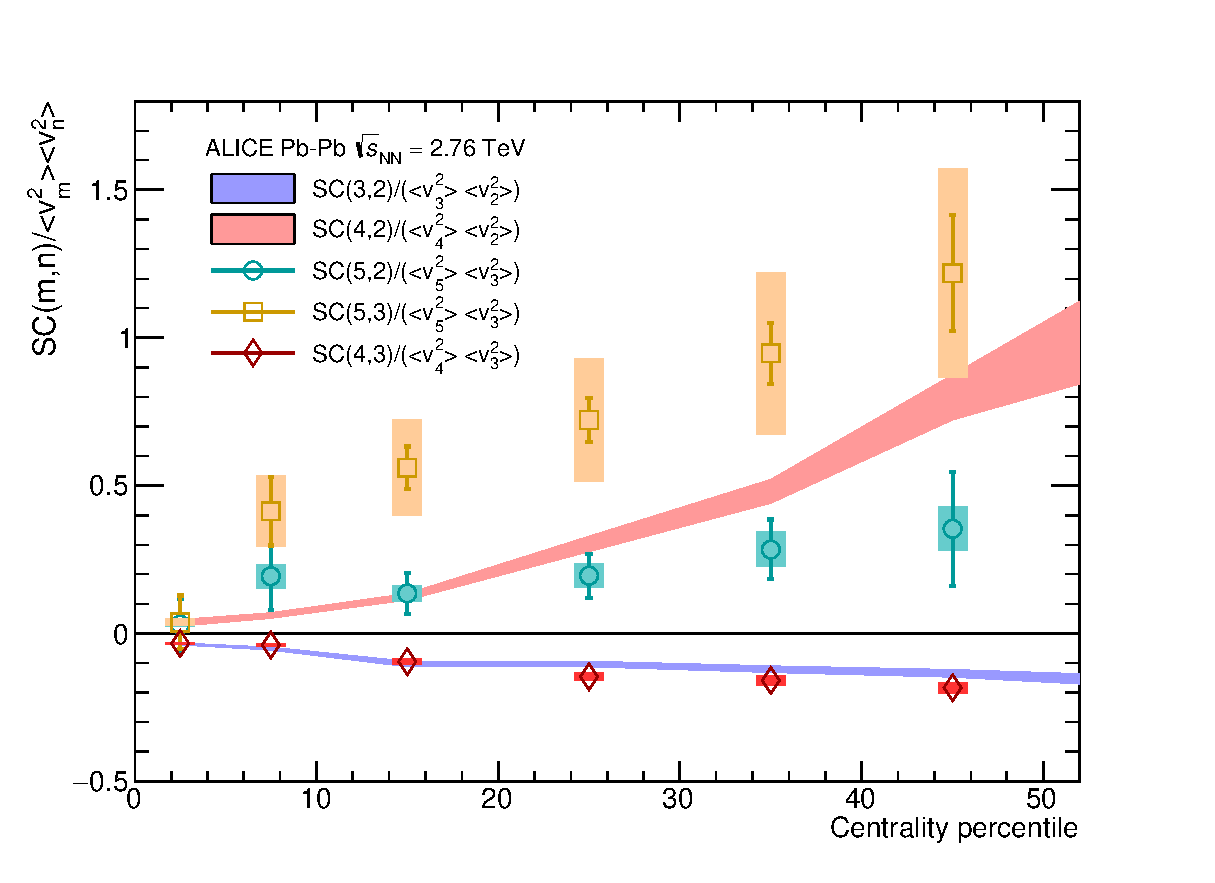
\includegraphics{figures/figs_results/fig2_QConly_higherNSC}}
        \caption{The results of $SC(m,n)$(upper figure) and $NSC(m,n)$(bottom figure) with higher order up to 5th flow harmonics with q-Cumulants method from ALICE Pb+Pb $\sqrt{S_{NN}}=2.76$~TeV. Note that The lower order $SC(m,n)$ are scaled down by 0.1. Both $SC(m,n)$ and $NSC(m,n)$ with lower orders are drawn as colored band and statistical and systematical errors were quadratically merged. }
        \label{fig:highersc}
        \end{center}   
     \end{figure}


As predicted as hydrodynamic calculation \cite{Bhalerao:2015jg} the correlation between $v_3^2$ and $v_4^2$ is negative and the others are positive. The correlation between higher harmonics ($v_3$ and $v_4$, $v_2$ and $v_5$, $v_3$ and $v_5$) become smaller for more central collisions, and it suggests that the correlation is likely due to the non-linear contributions of higher order flow harmonics like $v_4$ and $v_5$ \cite{PhysRevC.85.024908}. 

However, unlike $SC(m,n)$, $NSC(m,n)$ results with the higher order flow harmonics show almost same order of the correlation strength as the lower order flow harmonic correlations ($NSC(3,2)$ or $NSC(4,2)$). $NSC(4,3)$ is comparable to $NSC(3,2)$ and one finds that a hierarchy $NSC(5,3) > NSC(4,2) > NSC(5,2)$ holds for most of centrality ranges within the errors.
These results indicate that the lower oder harmonic correlations ($SC(3,2)$ and $SC(4,2)$) are larger than higher order harmonic correlations ($SC(4,3), SC(5,2)$, and $SC(5,3)$), not only because of the correlation strength itself but also the individual flow strength. 
$SC(5,2)$ is stronger than $SC(5,3)$, however as for $NSC$, the correlation between $v_5$ and $v_3$ is stronger than the correlation between $v_5$ and $v_2$. 


	\begin{figure}[h]
		\begin{center}
        	\resizebox{0.325\columnwidth}{!}{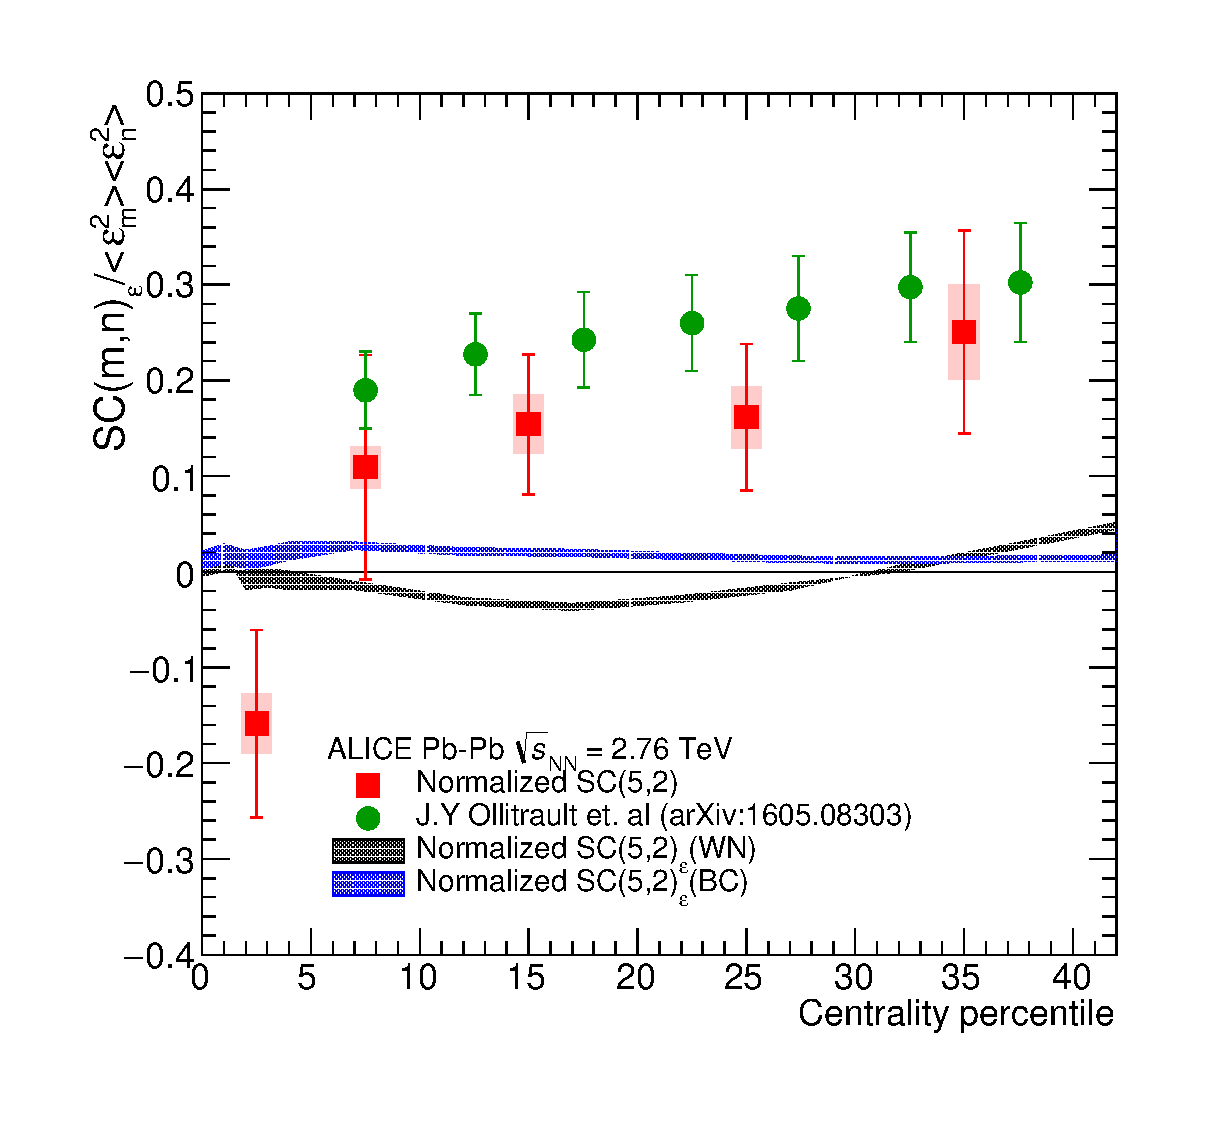
\includegraphics{figures/fig_ecen/SC_Comparison_ecen_BC_SC52}}
        	\resizebox{0.325\columnwidth}{!}{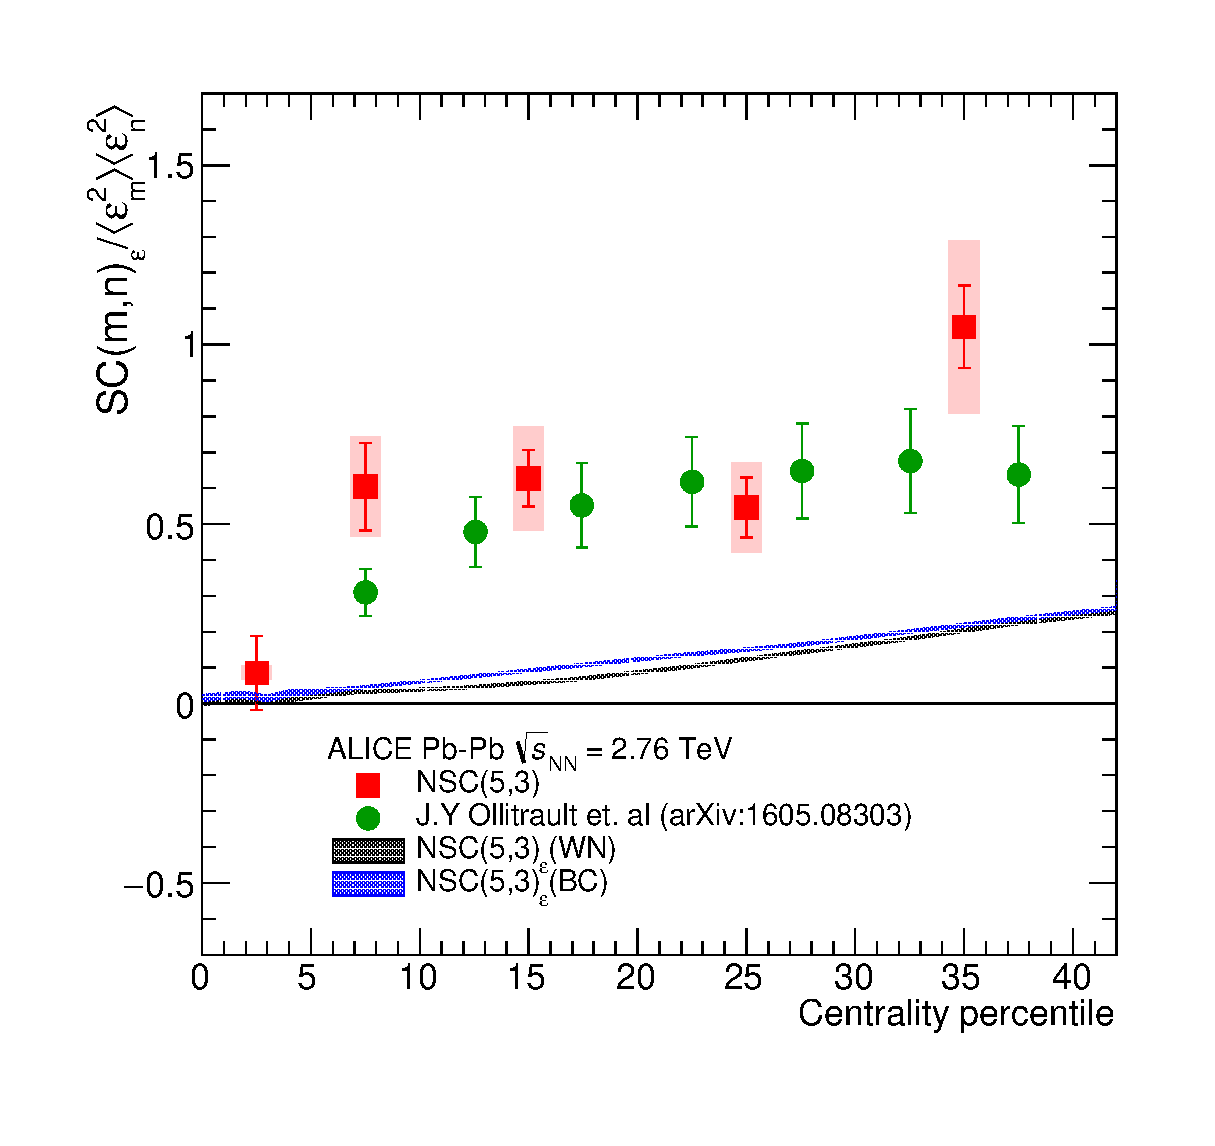
\includegraphics{figures/fig_ecen/SC_Comparison_ecen_BC_SC53}}
        	\resizebox{0.325\columnwidth}{!}{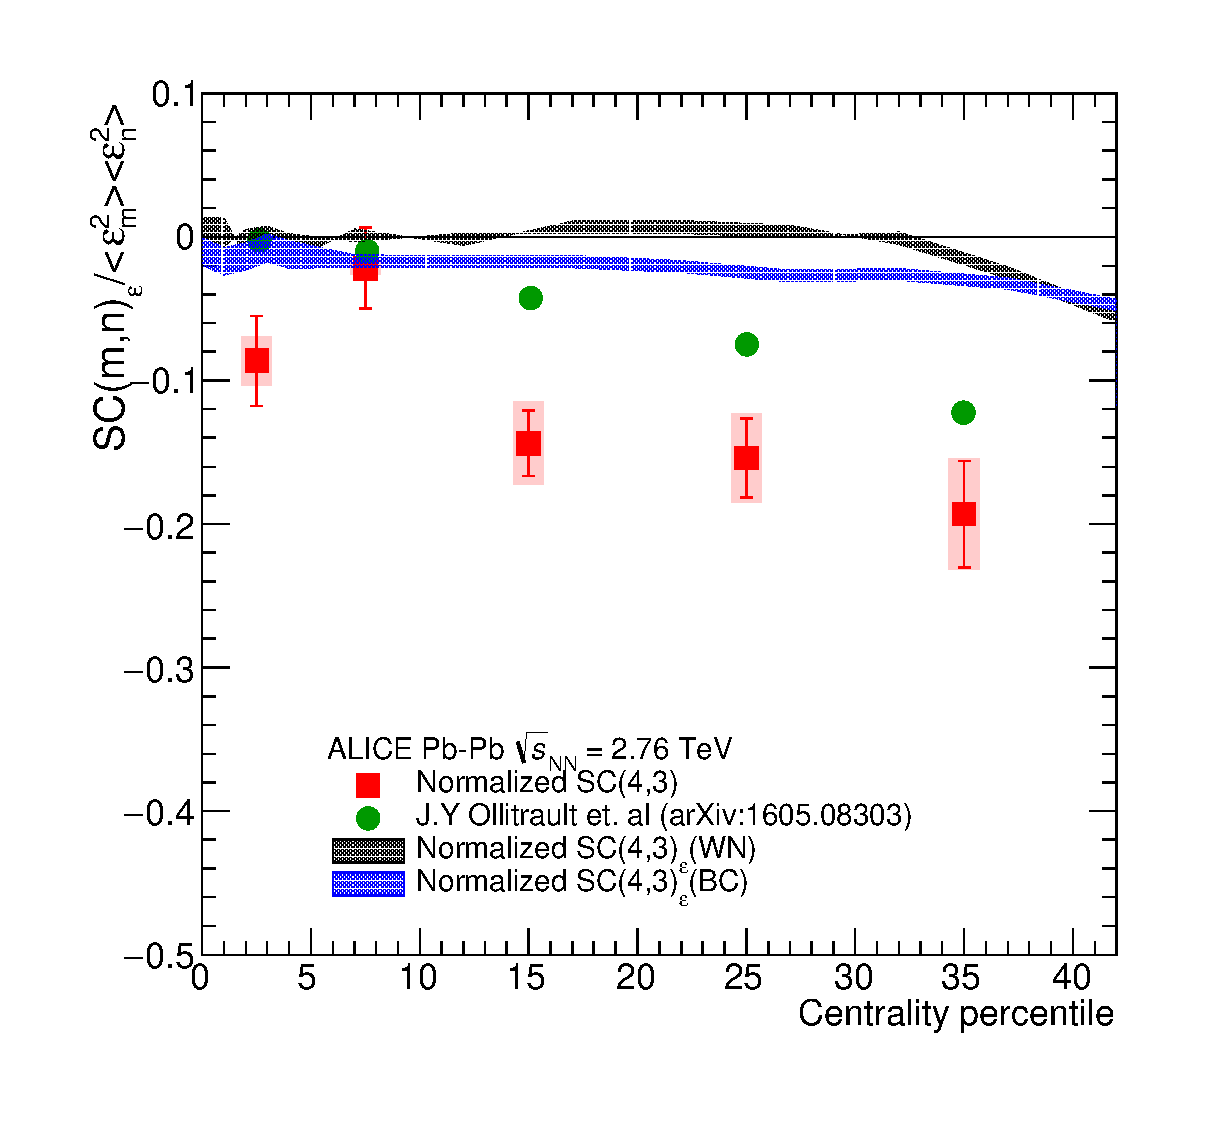
\includegraphics{figures/fig_ecen/SC_Comparison_ecen_BC_SC43}}
        \caption{The results of  higher order $NSC(m,n)$ and comparison to MC-Glauber models and prediction from J.Y Ollitraults\cite{Giacalone:2016afq}  }
        \label{fig_sc_higher:glauber}
        \end{center}   
     \end{figure}

 The $NSC(m,n)$ with higher order harmonics were compared to MC-Glauber to check the response (both linear and non-linear) of initial geometry. The $NSC(m,n)$ in coordinate space (as defined in Eq.\ref{eq:sc_ecen}) with both WN and BC weights were compared and shown in Fig.\ref{fig_sc_higher:glauber}. The large differences between MC-Glauber models (both WN and BC) and data shows that the correlation between flow harmonics can not be explained by only linear contribution of initial fluctuation. Also the prediction from J.Y Ollitraults from ALICE lower order $SC(m,n)$ and EP (Event Plane) correlation from ATLAS with few assumptions~\cite{Giacalone:2016afq} were shown together as green marker in Fig.\ref{fig_sc_higher:glauber}. Although it predict better than any other existing theoretical models, however still have some deviation between data for $NSC(4,3)$ case.
 

	\begin{figure}[h]
		\begin{center}
        	\resizebox{0.325\columnwidth}{!}{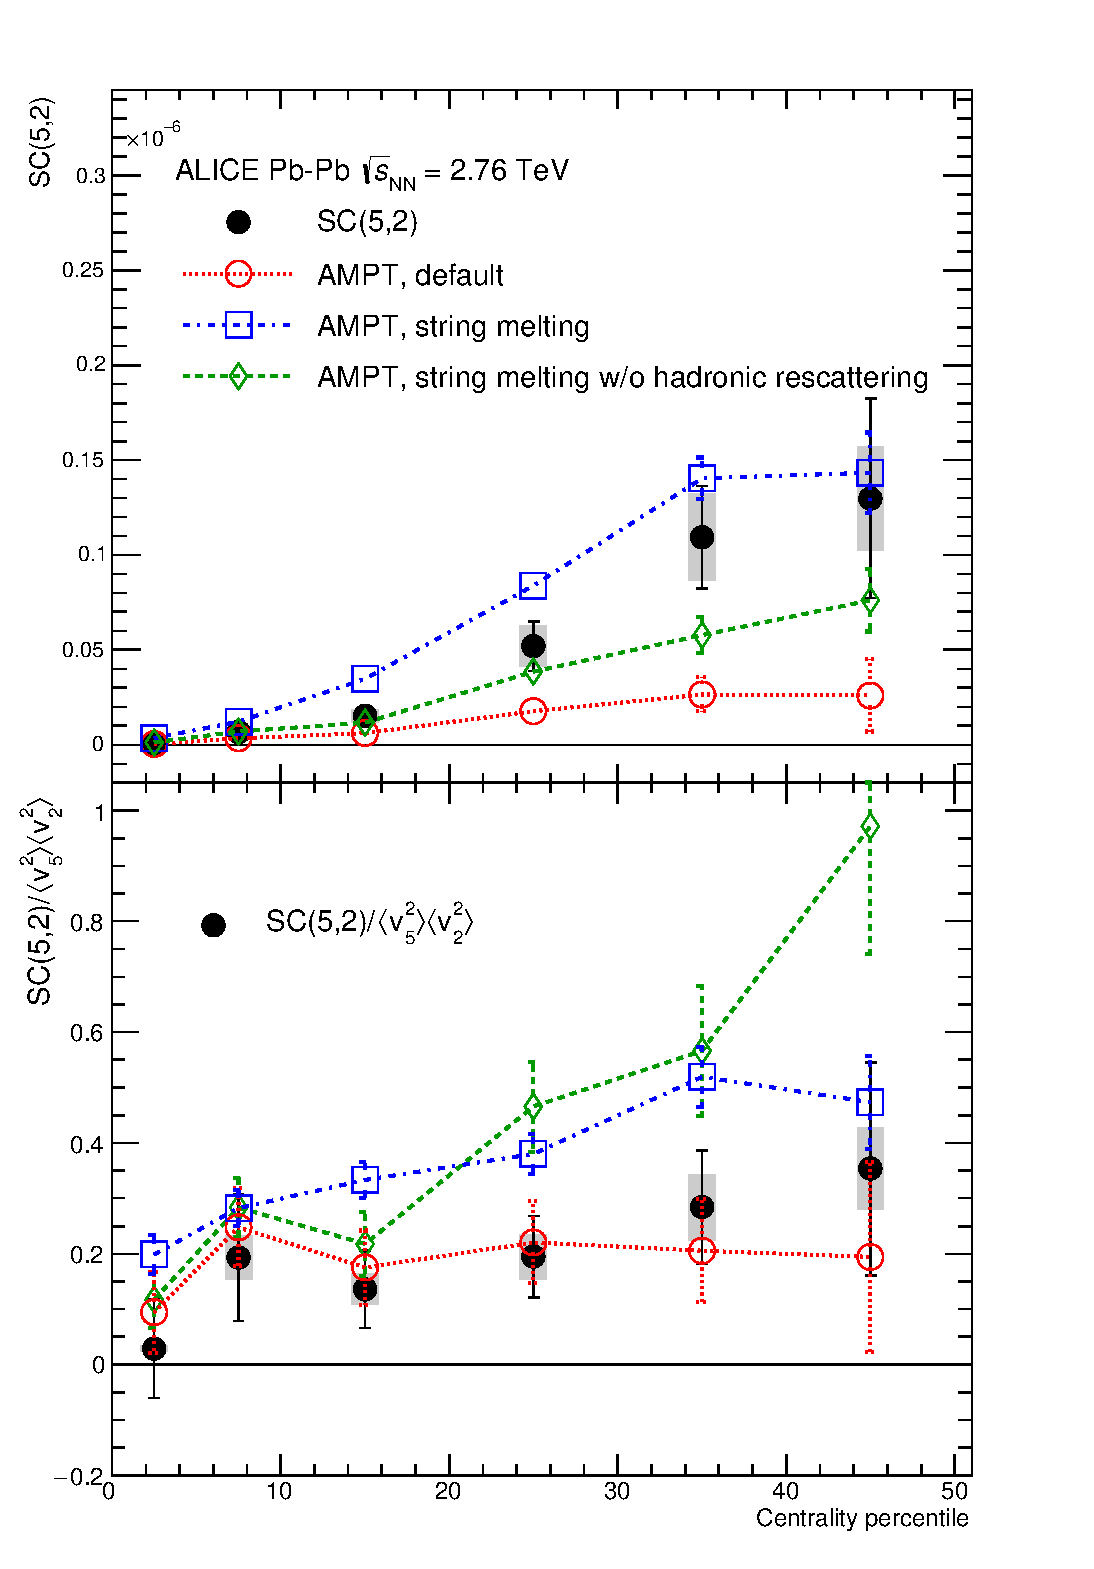
\includegraphics{figures/figs_results/fig3_QConly_ModelComparison_SC52_ampt.eps}}
        	\resizebox{0.325\columnwidth}{!}{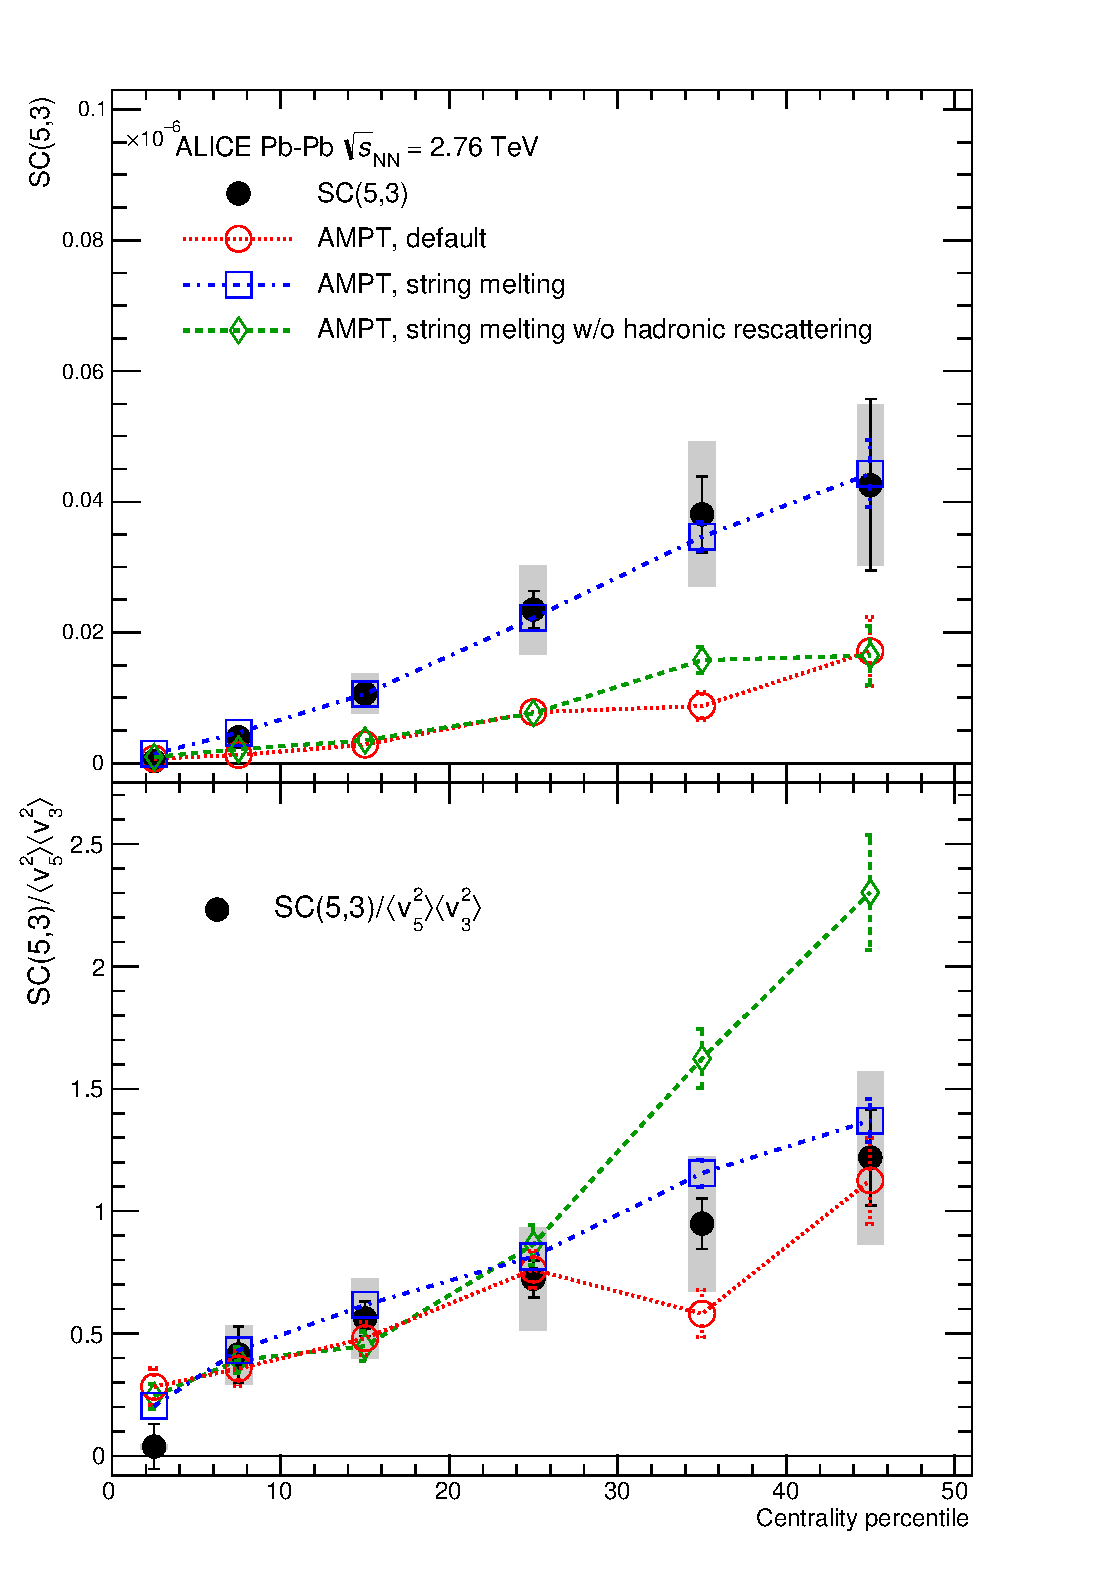
\includegraphics{figures/figs_results/fig3_QConly_ModelComparison_SC53_ampt.eps}}
        	\resizebox{0.325\columnwidth}{!}{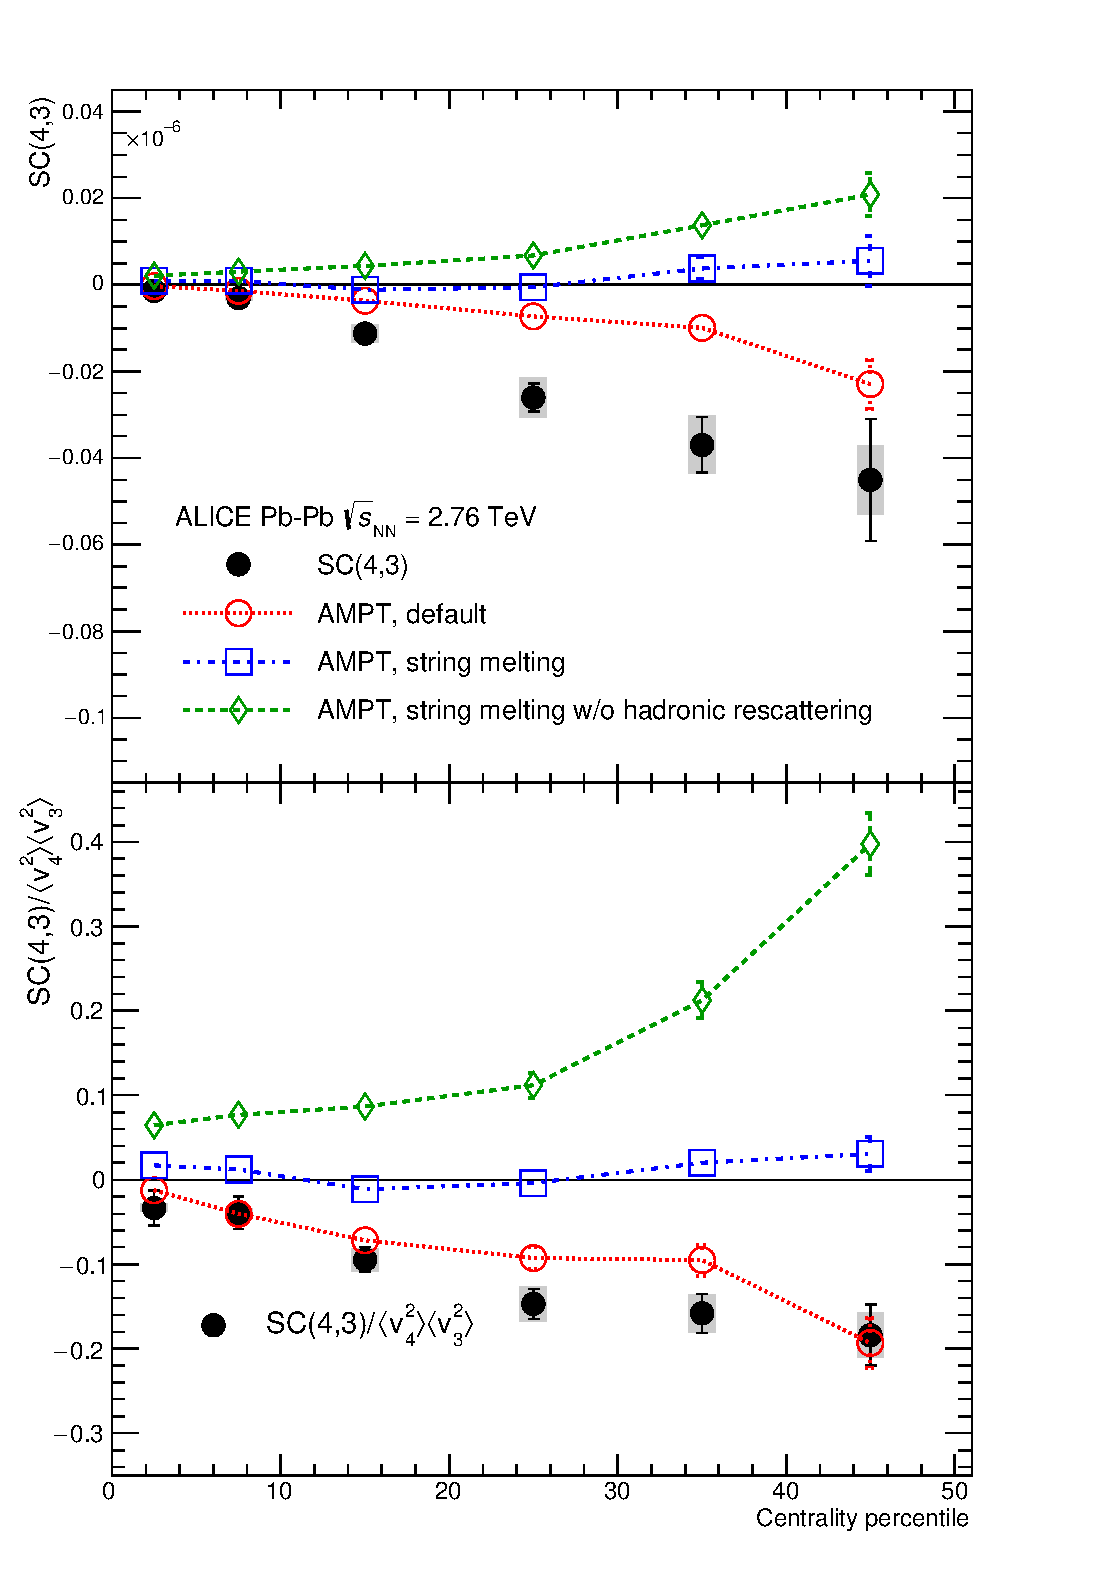
\includegraphics{figures/figs_results/fig3_QConly_ModelComparison_SC43_ampt.eps}}
        \caption{The results of  $SC(5,2)$, $SC(5,3)$ and $SC(4,3)$ and comparison to various AMPT simulations with different settings.  Upper figures are the results of $SC(m,n)$ and the lower figures are the results of $NSC(m,n)$}
        \label{AMPTcomhigh}
        \end{center}   
     \end{figure}
     
     
The extracted results  from particle level AMPT simulations in the same way as for the data are compared to the data in Fig.\ref{AMPTcomhigh}.
The string melting AMPT model describes SC(5,2) and SC(5,3) well. The same setting describes only $NSC(5,3)$. However, it overestimates $NSC(5,2)$. 
However the default AMPT model can describe $NSC(5,3)$ and $NSC(5,2)$ fairly well as similarly as $NSC(3,2)$ and $NSC(4,2)$.
In case of $SC(4,3)$, neither of the settings can describe the data but the default AMPT model follows the data closest. 
The string melting AMPT model fails to describe $SC(4,3)$ and $NSC(4,3)$.
In summary, the default AMPT model describes the normalized SC (NSC$(m,n)$) from lower to higher order harmonic correlation while the string melting AMPT model overestimates $NSC(5,2)$ and 
underestimates (or very week correlations) $NSC(4,3)$. 
     

	\begin{figure}[h]
		\begin{center}
        	\resizebox{0.325\columnwidth}{!}{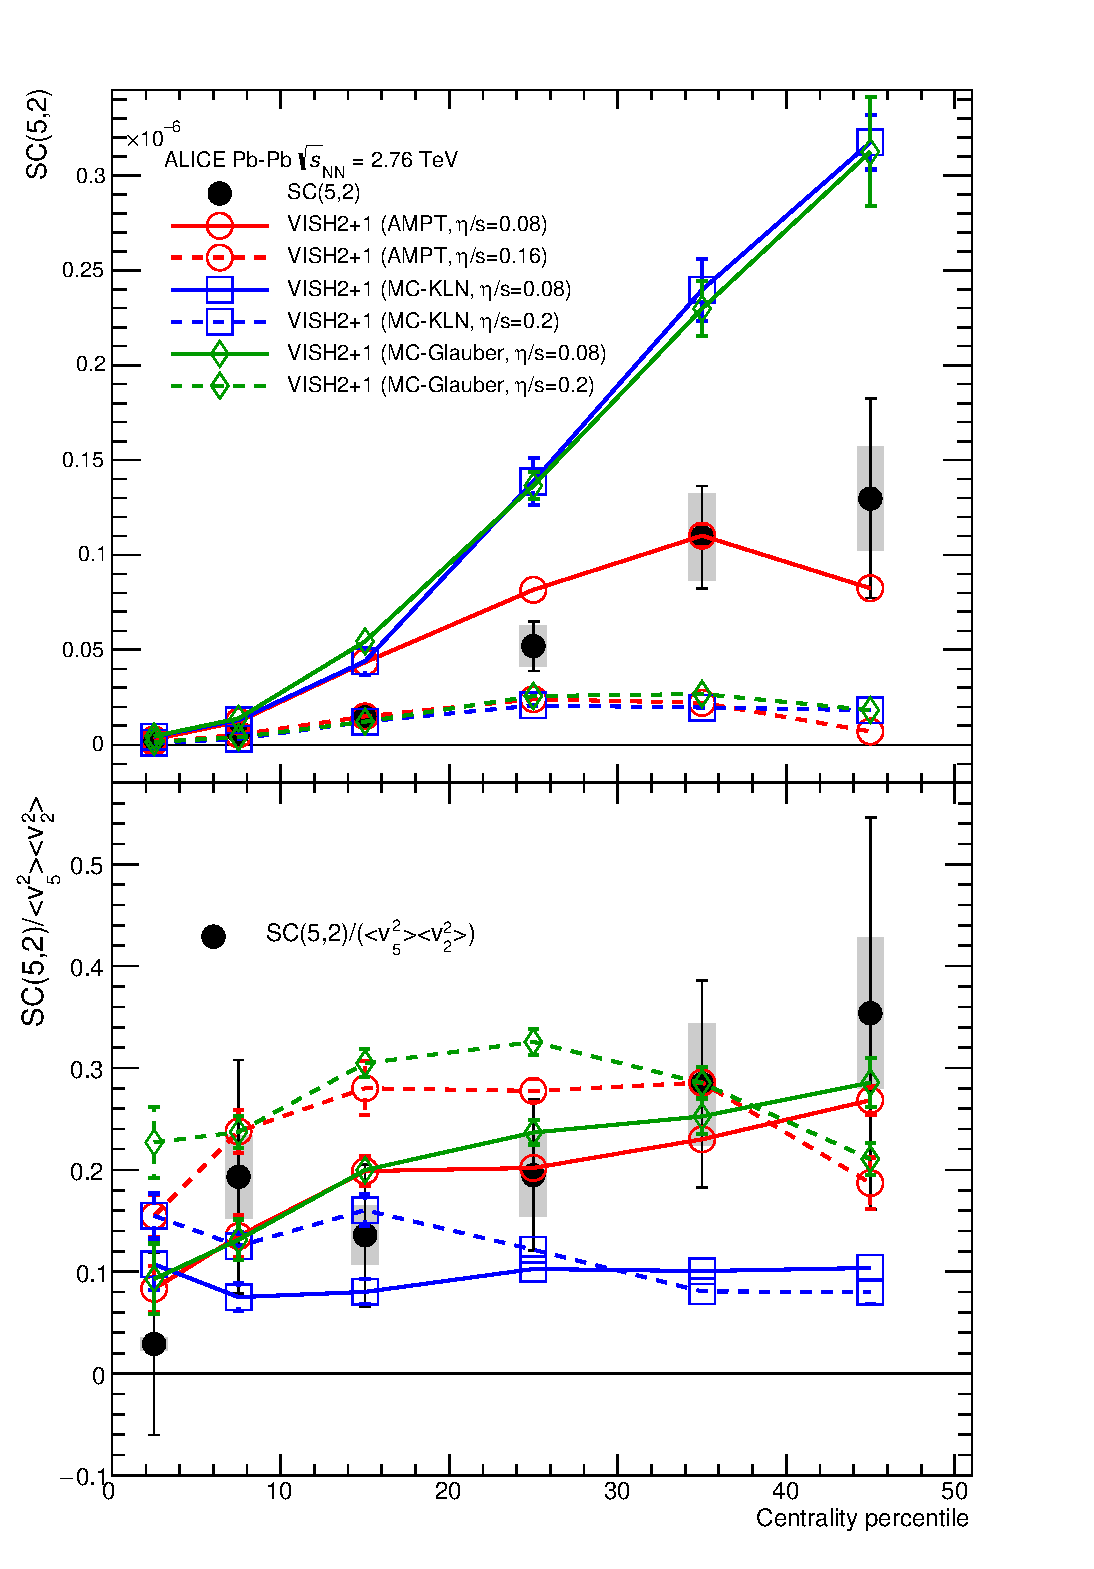
\includegraphics{figures/figs_results/fig3_QConly_ModelComparison_SC52_vish.eps}}
        	\resizebox{0.325\columnwidth}{!}{\includegraphics{figures/figs_results/fig3_QConly_ModelComparison_SC53_vish.eps}}
        	\resizebox{0.325\columnwidth}{!}{\includegraphics{figures/figs_results/fig3_QConly_ModelComparison_SC43_vish.eps}}
        \caption{Result of  $SC(5,2)$, $SC(5,3)$ and $SC(4,3)$ with ALICE data and comparison to various VISH2+1 calculation with different settings. The configurations are same as Fig.\ref{vish21}}
        \label{vishcomhigh}
        \end{center}   
     \end{figure}

  The event-by-event calculation from VISH by using a hybrid approach based on (2+1)-dimensional viscous hydrodynamics(VISH2+1) were tested and shown in Fig.\ref{vishcomhigh}. All the models with the large share viscosity regardless of the initial conditions ($\eta/s$=0.2 for MC-KLN and MC-Glauber initial conditions, and $\eta/s = 0.16$ for AMPT) failed to capture the centrality dependence of $SC(5,2), SC(5,2)$, and $SC(5,3)$ more clearly than lower order harmonic correlations ($SC(3,2), SC(4,2)$).
And among the models with small shear viscosity ($\eta/s$=0.08), the one from the AMPT initial condition describes the data much better than the other initial conditions. 
A quite clear separation between different initial conditions is observed for these higher order harmonics correlations compared to the lower order harmonic correlations.
$NSC(5,2)$ and $SC(5,3)$ are quite sensitive to both the initial conditions and the $\eta/s$ parametrizations.
As similarly as the above mentioned hydrodynamic calculations~\cite{Niemi:2015qia}, the sign of the $NSC(4,3)$ in these models is opposite to the data in 0-10\% central collisions. NSC(4,3) shows sensitivity to both initial conditions and $\eta/s$ parameterizations while $NSC(3,2)$ didn't show sensitivity to neither initial conditions nor $\eta/s$ parameterizations.
SC(4,3) data is clearly flavoured by smaller $\eta/s$ but NSC(4,3) cannot be described by these models quantitively.






\section{$p_{\rm{T}}$ dependence of $SC(m,n)$ and normalized $SC(m,n)$}

To analyze $p_{\rm{T}}$ dependence of $SC(m,n)$ and normalized $SC(m,n)$ result, we set various cut conditions for $p_{\rm{T}}$ of measuring particles, instead of using all charged hadrons with $0.2 < p_{\rm{T}} < 5.0$ GeV/$c$ in $|\eta|<0.8$ region. The simplest approach to analyze $p_{\rm{T}}$ dependence is to apply different $p_{\rm{T}}$ bin windows when measuring $SC(m,n)$. But the number of particles in each $p_{\rm{T}}$ bin groups decreases rapidly as function of $p_{\rm{T}}$ and the number of combination for cumulants pair will decrease even more rapidly ($ \sim\frac{1}{n^4}$) and this method causes large statistical fluctuations. Because the original $SC(m,n)$ has only the order of few $10^{-6}$ strength signal, it is not simple to get clear $p_{\rm{T}}$ dependence from different $p_{\rm{T}}$ window bins from a large statistical fluctuations. To prevent the statistical fluctuation issue, we apply minimum $p_{\rm{T}}$ cuts, instead of $p_{\rm{T}}$ bin-by-bin windows. In this analysis, we tested $SC(m,n)$s (and also $NSC(m,n)$s) with different $p_{\rm{T}}$ conditions from $0.2 \sim 5.0$GeV/$c$ to $1.5 \sim 5.0$GeV/$c$. 
%%done here

The result of $p_{\rm{T}}$ dependence with $SC(3,2)$ and $SC(4,2)$ is shown in Fig.\ref{fig:ptdep}. As seen in figure, the strength of $SC(m,n)$ correlation becoming larger as function of minimum $p_{\rm{T}}$. This indicates that the relationship between event-by-event fluctuation of two different flow harmonics $v_m$ and $v_n$ is stronger in high $p_{\rm{T}}$ region. This $p_{\rm{T}}$ dependence correlation is relatively small in central collision centralities and large in non-central collisions. However, this correlation between flow harmonics and $p_{\rm{T}}$ is not clearly shown in $NSC(m,n)$s. The  $NSC(m,n)$ results are aligned all together and consistent within errors. The ratio to default cut ($0.2 < p_{\rm{T}} < 5.0$GeV/$c$) is nearly 1 for all centrality. This suggests that the $p_{\rm{T}}$ dependence of $SC(m,n)$ are not solely comes from the correlation between flow harmonics but comes from the strength dependence of $p_{\rm{T}}$ of single $v_n$ values. Minimum $p_{\rm{T}}$ cuts are extended to 1.5 GeV/$c$ and the results are shown in Fig.\ref{fig:ptdephigh}. Even in higher minimum $p_{\rm{T}}$ cuts, there is no clear $p_{\rm{T}}$ dependence in normalized $SC(3,2)$ or $SC(4,2)$. For detail study of $p_{\rm{T}}$ dependence of  $NSC(m,n)$, the $NSC(m,n)$ as function of minimum $p_{\rm{T}}$ cuts are prepared in Fig.\ref{fig:SC_xpt}. Unlike AMPT prediction, the results from the data does not have clear $p_{\rm{T}}$ dependence up to 40\% collision centralities. In 40-50\% collision centrality region, there is a slightly decreased slope in $NSC(3,2)$ but it is not enough to say that there is $p_{\rm{T}}$ dependence for $NSC(3,2)$. For AMPT simulations, AMPT with string melting configuration failed to capture data result. These AMPT simulation predict that normalized $SC(m,n)$ increase as a function of minimum $p_{\rm{T}}$ and turns over to positive values around minimum $p_{\rm{T}} \sim 1.0$GeV/$c$. But in LHC10h data, the results remains in negative values for all minimum $p_{\rm{T}}$ bins, and centrality bins. Also for $NSC(4,2)$ cases, only AMPT default which has the configuration without string melting, has similar values with data. The others (AMTP with string melting) predict increase of $NSC(4,2)$ from around $\sim 1$GeV/$c$ minimum $p_{\rm{T}}$ cuts, and failed to reproduce the data.

	\begin{figure}[p]
		\begin{center}
        	\resizebox{0.6\columnwidth}{!}{\includegraphics{figures/figs_results/fig4_QConly_SC_ptdep}}
        	\resizebox{0.6\columnwidth}{!}{\includegraphics{figures/figs_results/fig4_QConly_nSC_ptdep}}
        	\resizebox{0.6\columnwidth}{!}{\includegraphics{figures/figs_results/fig4_QConly_nSC_ptdep_ratio}}
        \caption{The results of $SC(3,2)$ and $SC(4,2)$ with various minimum $p_{\rm{T}}$ cut conditions(Top) and results of  $NSC(3,2)$ and $NSC(4,2)$(Middle). The ratio of $NSC(m,n)$ results with various minimum $p_{\rm{T}}$ cut conditions to default($0.2 < p_{\rm{T}} < 5.0$~GeV/$c$ are shown in bottom figure.}
        \label{fig:ptdep}
        \end{center}   
     \end{figure}


	\begin{figure}[p]
		\begin{center}
        	\resizebox{0.6\columnwidth}{!}{\includegraphics{figures/figs_results/fig4b_QConly_SC_ptdep}}
        	\resizebox{0.6\columnwidth}{!}{\includegraphics{figures/figs_results/fig4b_QConly_nSC_ptdep}}
        	\resizebox{0.6\columnwidth}{!}{\includegraphics{figures/figs_results/fig4b_QConly_nSC_ptdep_ratio}}
        \caption{The results of $SC(3,2)$ and $SC(4,2)$ with various minimum $p_{\rm{T}}$ cut conditions(Top) and results of  $NSC(3,2)$ and $NSC(4,2)$(Middle). The ratio of $NSC(m,n)$ results with various minimum $p_{\rm{T}}$ cut conditions to default($0.2 < p_{\rm{T}} < 5.0$GeV/$c$ are shown in bottom figure.}
        \label{fig:ptdephigh}
        \end{center}   
     \end{figure}


	\begin{figure}[p]
		\begin{center}
        	\resizebox{0.95\columnwidth}{!}{\includegraphics{figures/figs_results/fig5_QConly_xminpt_nSC32}}
        	\resizebox{0.95\columnwidth}{!}{\includegraphics{figures/figs_results/fig5_QConly_xminpt_nSC42}}
           \caption{$NSC(3,2)$(Top) and $NSC(4,2)$(Bottom) as a function of minimum $p_{\rm{T}}$ cuts with ALICE Pb+Pb $\sqrt{S_{NN}}=2.76$TeV. The AMPT simulation results are drawn together as colored band for comparison. The corresponding AMPT configurations are shown in legend.}
        \label{fig:SC_xpt}
        \end{center}   
     \end{figure}
\clearpage

%done here


\section{Method comparison}


The Eq.\ref{eq:SC} is based on the multi-particle q-Cumulants method(i.e. QC method), but it can be also obtained by calculating moments \cite{Bhalerao:2015jg} as discussed in the previous section\ref{sec:analysis}.


	\begin{figure}[bp]
		\begin{center}
        	\resizebox{0.47\columnwidth}{!}{\includegraphics{figures/figs_compare_with_SP/fig1a}}
        	\resizebox{0.47\columnwidth}{!}{\includegraphics{figures/figs_compare_with_SP/fig1b.eps}}
        \caption{Comparison of $SC(m,n)$(Top) and $NSC(m,n)$(Bottom) results for $SC(3,2)$(blue) and $SC(4,2)$(red) with the SP and QC method up to 60\% centralities. The different ratios are shown in lower pads, and systematic uncertainty is drawn as a band around 1}
        \label{SC_compare}
        \end{center}   
     \end{figure}


As seen in Fig.\ref{SC_compare} in both methods, the flow harmonics with 2nd and 4th are correlated. On the other hand, 2nd and 3rd harmonics are anti-correlated. The strength of correlation is small in the central collision region and becomes stronger in non-central collision in both q-Cumulant method(QC) and Scalar Product method(SP). Also  $NSC(m,n)$ which is divided by products $\langle v_m^2 \rangle \langle  v_n^2\rangle$, in order to obtain the normalized observables are shown and suggests the same trend but a large deviation especially for $SC(4,2)$. HIJING simulations results from SP methods are shown together for comparison. 

The advantage of using the SP method is that calculations are much simpler and faster in estimating the correlation between flow harmonics. Instead of calculating particle pair of 4- or 2- cumulants, the SP method needs only one calculation between measured n$^{th}$ order flow $Q$-vector. The other advantage of the SP method is that it can be applied for not only $SC(m,n)$ which observables for flow ``magnitudes" correlation, but also for the flow "direction" correlations like event-plane correlation. \cite{Aad:2014fla} or non-linear response of flow harmonics \cite{Yan:2015dh}. 

However, the disadvantage of SP methods is (likely) under estimation of $SC(m,n)$ in low multiplicity regions. This effects were discussed with ToyMC simulation in Appendix A. Because of this issue of difference between two different methods and inaccuracy(under estimation) of SP method in low multiplicity regions, we used all the result from QC method as the default in this analysis.


\subsubsection{Method comparison of higher order harmonics}


Also $SC(m,n)$ and $NSC(m,n)$ results with higher order flow harmonics (up to 5th order) were measured by the SP method, and the results are shown in Fig.\ref{SC_higherorder_comparison}. For the higher order, because of statistical fluctuation for peripheral collisions, results were only taken from the 0\% to 40\% collision centrality regions. As a result, the two methods shows the consistent values within errors.


	\begin{figure}[h]
		\begin{center}
        	\resizebox{0.65\columnwidth}{!}{\includegraphics{figures/figs_compare_with_SP/fig2b_1}}
        	\resizebox{0.65\columnwidth}{!}{\includegraphics{figures/figs_compare_with_SP/fig2b_2}}
        \caption{Result of higher order $SC(m,n)$ and $NSC(m,n)$ with two different method QC and SP. Along x-axis offset was applied for better visibility. For the QC method $|\eta| < 0.8$ cut was applied, while SP method takes $0.4 < |\eta| <0.8$.}
        \label{SC_higherorder_comparison}
        \end{center}   
     \end{figure}
     
     
\subsubsection{$p_{\rm{T}}$ dependence of $SC(m,n)$ with SP method}


  The $p_{\rm{T}}$ dependence of $SC(m,n)$ and $NSC(m,n)$ were checked with the SP method. The results of $SC(m,n)$ and $NSC(m,n)$ with different minimum $p_{\rm{T}}$ cuts are shown in Fig.\ref{fig:SC_pt_withSP_lower}( up to 0.7 GeV/$c$ minimum $p_{\rm{T}}$ cuts) and Fig.\ref{fig:SC_pt_withSP_higher}( up to 1.5 GeV/$c$ ) minimum $p_{\rm{T}}$ cuts. As seen in Fig.\ref{fig:SC_pt_withSP_lower}, there is certain $p_{\rm{T}}$ dependence for $SC(m,n)$, but not clear $p_{\rm{T}}$ dependence for  $NSC(m,n)$ as like QC method. However, in even higher $p_{\rm{T}}$ region(Fig.\ref{fig:SC_pt_withSP_higher}), unlike the results with QC methods, we could see weak $p_{\rm{T}}$ dependence in  $NSC(m,n)$. In the $SC(m,n)$ results, as the minimum $p_{\rm{T}}$ cuts goes higher, the strength of the correlation becomes stronger in both $SC(3,2)$ and $SC(4,2)$. However, in $NSC(m,n)$ with the SP method, when the minimum $p_{\rm{T}}$ cuts increase, the strength of correlation for $NSC(3,2)$ is (negatively) stronger, but the strength of correlation of $NSC(4,2)$ becomes weaker. As a result, in higher $p_{\rm{T}}$ range, the $NSC(m,n)$ values always getting smaller.


	\begin{figure}[htbp]
            \begin{center}
                       \resizebox{0.84\textwidth}{!}{\includegraphics{figures/figs_compare_with_SP/fig3a.eps}}
                       \resizebox{0.84\textwidth}{!}{\includegraphics{figures/figs_compare_with_SP/fig3b.eps}}
              \end{center}
              \caption{$SC(m,n)$ and $NSC(m,n)$ with SP method with default cuts ( 0.2 < $p_{\rm{T}}$ < 5.0 GeV/$c$ ) and various minimum $p_{\rm{T}}$ cuts up to 0.7 GeV/$c$ }
              \label{fig:SC_pt_withSP_lower}
       \end{figure}


	\begin{figure}[htbp]
            \begin{center}
                       \resizebox{0.84\textwidth}{!}{\includegraphics{figures/figs_compare_with_SP/fig3a_higherpt.eps}}
                       \resizebox{0.84\textwidth}{!}{\includegraphics{figures/figs_compare_with_SP/fig3b_higherpt.eps}}
              \end{center}
              \caption{$SC(m,n)$ and $NSC(m,n)$ with SP method with default cuts ( 0.2 < $p_{\rm{T}}$ < 5.0 GeV/$c$ ) and various minimum $p_{\rm{T}}$ cuts up to 1.5 GeV/$c$ )}
              \label{fig:SC_pt_withSP_higher}
       \end{figure}



	\begin{figure}[htbp]
            \begin{center}
                                     \resizebox{0.84\textwidth}{!}{\includegraphics{figures/figs_compare_with_SP/fig3c.eps}}
                                     \resizebox{0.84\textwidth}{!}{\includegraphics{figures/figs_compare_with_SP/fig3c_higherpt.eps}}
              \end{center}
              \caption{ The ratio of $NSC(m,n)$ with SP method to the default cuts }
              \label{fig:SC_pt_withSP_ratio}
       \end{figure}

  For the better comparison, the ratio of normalized $SC(m,n)$ with various minimum $p_{\rm{T}}$ cuts to default is shown in Fig.\ref{fig:SC_pt_withSP_ratio}. Up to 0.7 GeV/c, the ratio of $NSC(m,n)$ values are consistent with a default cut within errors, but the minimum $p_{\rm{T}}$ exceeds 0.8GeV/c, the ratio of $NSC(3,2)$ moving above the 1, and the ratio of $NSC(4,2)$ goes down below the 1. The reason why these trends are only shown in the SP method, and not in the QC is not yet fully explained. However, the disadvantage of the SP method is that we lose almost half of the statistics because of a large $\eta$ gap around $\eta=0$ and also the number of combinations for the track pair is $\frac{1}{3}$ when compared to QC methods. This is one possible option to explain these $p_{\rm{T}}$ dependence behavior of SP method, and  tested in ToyMC simulation in Appendix A.


\clearpage
% !TEX root = main_org.tex


\chapter{Conclusion and Outlook}

As the strong evidence of QGP, flow has been studied in detail during the past few decades. But only a few studies have been done about correlation between flow harmonics and leads to the following questions; How do $v_n$ and $\epsilon_n$ fluctuate and what is the underlying probability density function ($p.d.f$) of their distribution? How are the initial geometry fluctuations reflected in differential flow measurements? What is the relationship between different harmonic event plane angle? What is the relationship between the flow coefficient of different harmonics? The answers to above questions (especially for the last) \textit{Symmetric Cumulants} ($SC(m,n)$) have been introduced as the key observable to measure correlation between flow harmonic ``magnitudes" $v_m$ and $v_n$.



As the result of $SC(m,n)$, We have found that fluctuations of $v_2$-$v_3$ and $v_3$-$v_4$ are anti-correlated in all centralities while fluctuations of $v_2$-$v_4$, $v_2$-$v_5$ and $v_3$-$v_5$ are correlated for all centralities. The various hydrodynamic calculations and model simulations were studied together as a reference. The large differences between data and MC-Glauber studies confirmed that the correlation were not able to explained by only linear response of initial conditions, and there is certain non-linear contribution of initial fluctuations. The analysis with higher order flow harmonics provides that the correlation between higher order flow harmonics and lower order harmonics is likely due to the non-linear contributions. It  also indicates that the higher order flow can be understood as the superposition of the lower order flow harmonics. This analysis will help constrain the theoretical description of the fluid close the freeze-out temperature which is probably the least understood part of hydrodynamic calculation. \cite{Teaney:2012ke} \cite{Yan:2015dh}

 None of the existing models and hydrodynamic calculation with the different parameterizations of the temperature dependence of $\eta/s$ couldn't exactly capture the data quantitatively. Furthermore, the sign of $v_3$-$v_2$ correlation in most central collision range(0-10\%) was found to be different between the data and hydrodynamic model calculations.  In the most central collisions the anisotropies originate mainly from fluctuations, i.e. the initial ellipsoidal geometry characteristic for mid-central collisions plays little role in this regime.  Hence this observation might help to understand the details of the fluctuations in initial conditions.
 
 It is suggested that the $SC(m,n)$ is more sensitive to both initial conditions and hydrodynamic property $\eta/s$ than single flows.  In addition, we have found that the different order harmonic correlations have different sensitivities to the initial conditions and the system properties. Therefore they have discriminating power on separating the role of the $\eta/s$  from the initial conditions to the final state particle anisotropies.

The comparisons to VISH2+1 calculation show that all the models with large $\eta/s$ regardless of the initial conditions failed to capture the centrality dependence of higher order correlations, more clearly than lower order harmonic correlations. 
Based on the tested model parameters, the $\eta/s$ should be small and AMPT initial condition is favored by the data. A quite clear separation of the correlation strength between different initial conditions is observed for these higher order harmonic correlations compared to the lower order harmonic correlations.

We have found that $v_3$-$v_2$ and $v_4$-$v_2$ correlations have moderate $p_{\rm T}$ dependence in mid-central collisions. This might be an indication of possible viscous corrections for the equilibrium distribution at hadronic freeze-out.
The results presented in this article can be used to further optimize model parameters and put better constraints on the initial conditions and the transport properties of nuclear matter in ultra-relativistic heavy-ion collisions. However, the $p_{\rm{T}}$ dependences in $NSC(m,n)$ are not shown clearly.

We introduced the Scalar Product method (SP method) to measure $SC(m,n)$ and  $NSC(m,n)$, and checked with the results from QC method. Basically, most of the results are consistent in errors. However at some points, there are some deviations between the SP and QC methods. These differences are most pronounced in peripheral collision centrality regions. We investigate the reason of difference between two methods by testing and measuring $SC(m,n)$ with ToyMC, and PYTHIA jet implementation, but not able to fully explain the differences. 
At this point, we are not sure whether different methods respond differently to flow fluctuations or if we can rule out non-flow effects in the end. The answer might provide a hint for different sensitivities to flow fluctuations and non-flow effect. This might be a nice piece of material by itself in further study.

Even though, there are some missing parts on this analysis, such as no clear $p_{\rm{T}}$ dependence of  $NSC(m,n)$ and absence of explanation for different method response, it provides quantitative hints for the comprehensive understanding of hydrodynamical behavior of collide system evolution. Also new observables $SC(m,n)$ promise to provide additional constraints on the initial state phenomena and dynamical evolution and its fluctuation without event-by-event shape engineering. Since Run2 data from LHC is approaching with a new highest record of center-of-mass energy and much higher amount of events, more interesting analysis including correlations and fluctuations will be studied again.




\clearpage
\begin{appendices}
% !TEX root = main_org.tex

\chapter{Toy MC simulation}

\subsection{Toy Monte Calro simulation}
In this appendix, we will the Monte Carlo simulation to check the correlation between two different flow harmonics and check the systematics response to $Q$-Cumulant method(QC) and Scalar Product method(SP). 

\smallskip	
	
	Since, $SC(m,n)$ is defined as like $$ \langle v_n^2 v_m^2 \rangle - \langle v_n^2 \rangle \langle v_m^2 \rangle $$
	it is not easy to calculate directly $SC(m,n)$ from arbitary $v_n$ and $v_m$ which fluctuate event by event. So, in this Toy Monte Calro simulation, we consider simplest case. i.e the uniform flow distribution.
	The uniform flow distribution is defined as like
	
	\begin{equation}
		f(v_n) = const, \hskip5mm v_{min} < v_n < v_{max}
	\end{equation}
	
	In this configuration, we can easily assume that the function of flow $v_n$ can be normalized with
	
	\begin{eqnarray}
		1 &=& \int_{-\infty}^{\infty}f(v_n)dv \\
			&=& \int_{v_{min}}^{v_{max}}const ~ dv \\
			&=& cont (v_{max} - v_{min} )
	\end{eqnarray}
	
	
	so,
	\begin{equation}
		const = \frac{1}{v_{max} - v_{min} }
	\end{equation}
	\smallskip
	
	Then the final normalized unifrom flow distribution is
	\begin{equation}
		f(v_n) = \frac{1}{v_{max} - v_{min}}
	\end{equation}
	\smallskip
	
	And if we assume the mean value of given order flow harmonics as $\mu_v$, then it follows
		
		
	\begin{eqnarray}
		1 &=& \int_{-\infty}^{\infty}vf(v)dv \\
			&=& \int_{v_{min}}^{v_{max}} v \frac{1}{v_{max} - v_{min}}  dv \\
			&=& \frac{1}{v_{max} - v_{min}} \frac{v_{max}^2 - v_{min}^2}{2}
	\end{eqnarray}

	and finally we have 
	
	\begin{equation}
		\mu_v = \frac{v_{max} - v_{min}}{2}
	\end{equation}
	\smallskip
	
	To calculated standard deviation($\sigma_v$) for event fluctuations, use the definiation of expectaion value of a random variables.
	
	\begin{equation}
		\mu_x = E[x] = \int_{-\infty}^{\infty}{xf(x)dx}
	\end{equation}
	\begin{equation}
		\sigma_x^2 = V[x] = E[(x-E[x])^2] = \int_{-\infty}^{\infty}{(x-\mu_x)^2 f(x) dx}
	\end{equation}
	\smallskip
	
	So, we can get straightforwardly
	
	\begin{equation}
		\sigma_v^2 = \frac{1}{12}(v_{max} - v_{min})^2
	\end{equation}
	
	or,
	
	\begin{equation}
		\sigma_v = \frac{1}{2\sqrt{3}}(v_{max} - v_{min})
	\end{equation}
	\smallskip
	
	
	So, for the uniform distribution Toy models, we can express the flow $v_n$ and its fluctuation with events($\sigma_v$) as term as uniform flow distribution ($v_{max}$ and $v_{min}$)
	
	\begin{equation}
		\langle v \rangle = \frac{v_{max} + v_{min}}{2}
	\end{equation}
	\begin{equation}
		\langle v^2 \rangle = \frac{v_{max}^2 + v_{max}v_{min} + v_{min}^2}{3}
	\end{equation}
	\begin{equation}
		\langle v^3 \rangle = \frac{1}{4} (v_{max} + v_{min})(v_{max}^2 + v_{min}^2 )
	\end{equation}	
	\begin{equation}
		\langle v^4 \rangle = \frac{1}{5}(v_{max}^4 + v_{max}^3v_{min} + v_{max}^2v_{min}^2 + v_{max}v_{min}^3 + v_{min}^4)
	\end{equation}
	\smallskip
	
	With above equations, we now can express the $SC(m,n)$ as term of $v_{max}$ and $v_{min}$ only. For example, if we set $v_2$ and $v_3$ to have uniform distribution such as
	
	\begin{itemize}
	\item $v_2$ = Uniform[0.05, 0.08]
	\item $v_3 = 0.1 - v_2$
	\end{itemize}
	
	then the $SC(3,2)$ will be express as like 
	\begin{eqnarray}
		SC(3,2) &=& \langle v_3^2 v_2^2 \rangle - \langle v_3^2 \rangle \langle v_2^2 \rangle \\
		&=& \langle x^2 (0.1-x)^2 \rangle - \langle x^2 \rangle \langle (0.1-x)^2 \rangle \\
		&=& \langle x^2(0.01 - 0.2x + x^2 ) \rangle - \langle x^2 \rangle \langle (0.01 - 0.2x + x^2 ) \rangle \\
		&=& \langle 0.01x^2 \rangle - \langle 0.2x^3 \rangle + \langle x^4 \rangle - \langle x^2 \rangle ( 0.01 - \langle 0.2 x \rangle + \langle x^2 \rangle ) \\
		&=& - (0.2)\langle x^3 \rangle + \langle x^4 \rangle + 0.2 \langle x \rangle \langle x^2 \rangle - \langle x^2 \rangle^2 \\
		&=& -(0.2) \frac{1}{4}(v_{max}+v_{min})(v_{max}^2 + v_{min}^2) \nonumber \\
		&& +\frac{1}{5}(v_{max}^4 + v_{max}^3v_{min} + v_{max}^2v_{min}^2 + v_{max}v_{min}^3 + v_{min}^4)  \nonumber\\
		&& 0.2\frac{v_{max}^2 + v_{max}v_{min} + v_{min}^2}{3} \frac{v_{max}+v_{min}}{2} \nonumber \\
		&& - \frac{v_{max}^2 + v_{max}v_{min} + v_{min}^2}{3}\frac{v_{max}^2 + v_{max}v_{min} + v_{min}^2}{3}
	\end{eqnarray}

 As a results $SC(3,2) \simeq -6.78 \times 10^{-7}$, Also $SC(4,2)$ can be obtained by similar calculations.

In this analysis, we tested with ToyMC simulation for $SC(m,n)$ with both uniform fluctuation case (which is simplest case), and 2-Dim Gaussian fluctuation case (which is more realistic case)
\smallskip
For the uniform fluctuation case, we set $v_n$ as like 
\begin{itemize}
	\item $v_2$ = Uniform[0.04, 0.09]
	\item $v_3$ = 0.1 - $v_2$
	\item $v_4$ = $v_2$ - 0.02	
\end{itemize}

These settings are based on the real flow measurements to have $\langle v_2 \rangle \sim 0.065$  which is similar $v_2$ in mid-central collisions, and setting $v_3$ to have negative correlation with similar as what it is measured. Also $v_4$ have been setted to have positive correlation but a little bit higher than what is measured.
	
\begin{figure}[h]
\begin{center}
\includegraphics[width=9.0cm]{figures/5tev_vns}
\caption{Flow measurement with ALICE at $\sqrt{S_{NN}} =  2.76$TeV/$c$ and $ 5.02$TeV/$c$ with various measurement methods, also hydrodynamic predictions are drwan as bands}
\label{vn5}
\end{center}
\end{figure}

We performed ToyMC simulations with various multiplicity and run over 1M events per each multiplicity bins. The results are shown in Fig.\ref{fig:ToyMC_Uniform_SC32_woJet} and  \ref{fig:ToyMC_Uniform_SC42_woJet}. As seen in results, both Q-cumulants (QC) and Scalar Product (SP) method were able to capture input value in high multiplicity regions with in $\sim1\%$ errors, but in low multiplicity region, we observe discrepancy between two methods and these effects are most pronounced in lowest multiplicity (corresponding to values for peripheral collisions over 60\% centrality). Neither QC nor SP methods were fully free from these effects. However, because of $\eta$ gap, SP method has disadvantages for the number of combinations(or multiplicity). As the result, QC methods recover better the input value than SP method, and SP method results are always smaller than QC for all multiplicity bins.   
	
\begin{figure}[h]
\centerline{\includegraphics[width=7.0cm]{figures/figs_ToyMC/SC_Comparison_SC32_ToyMC_low_woJet}
\includegraphics[width=7.0cm]{figures/figs_ToyMC/SC_Comparison_SC32_highonly_ToyMC_woJet}}
\caption{Results of ToyMC simulation for SC(3,2) with random uniform distribution of $v_n$ with various multiplicity. The left figure is the result from 50 to 450 multiplicity, and right figure is the result from 500 to 1800 multiplicity. Both Q-cumulatns(QC) and Scalar Product(SP) mehtods are tested and drawn with red and blue color marker. Also ratio to input values are drawn in bottom pad, and the ratio of SP / QC methods are drawn with green marker}
\label{fig:ToyMC_Uniform_SC32_woJet}
\end{figure}


\begin{figure}[h]
\centerline{\includegraphics[width=7.0cm]{figures/figs_ToyMC/SC_Comparison_SC42_ToyMC_low_woJet}
\includegraphics[width=7.0cm]{figures/figs_ToyMC/SC_Comparison_SC42_highonly_ToyMC_woJet}}
\caption{Results of ToyMC simulation for SC(4,2) with random uniform distribution of $v_n$ with various multiplicity. The left figure is the result from 50 to 450 multiplicity, and right figure is the result from 500 to 1800 multiplicity. Both Q-cumulatns(QC) and Scalar Product(SP) mehtods are tested and drawn with red and blue color marker. Also ratio to input values are drawn in bottom pad, and the ratio of SP / QC methods are drawn with green marker}
\label{fig:ToyMC_Uniform_SC42_woJet}
\end{figure}



Also we tested with 2-dim Gaussian like flow fluctuations to try a realistic flow fluctuation taken from a measured distribution.

\begin{equation}
p\left(v_n\right) = \frac{v_n}{\sigma^2}e^{-{\frac{v_n^2}{2\sigma^2}}},
\label{eq:gaussproj1}
\end{equation}

This is the radial projection of a 2 dimensional Gaussian distribution in $\bar v_n$. The $\sigma$ parameter is given by $\sigma=\sqrt{2/\pi}\left<v_n\right>$

then the settings are as like followings
\begin{itemize}
	\item $v_2$ = Bessel Gaussian (mean 0.065)
	\item $v_3$ = 0.04 - ($v_2$/8)
	\item $v_4$ = $v_2 / 6$ 
\end{itemize}

We set $v_n$ to have similar values in real flow values and to have $\sim SC(m,n)$ in mid centralities in ALICE data. The results are shown in Fig.\ref{fig:ToyMC_Gaus}. As same as uniform flow distribution case both method recover input values well and consistent in $1\%$ levels. However when we see the details, we can check that the results from SP methods are always lower than QC methods as like previous results. As the results, the ratio of SP over QC results are above 1 in $SC(3,2)$ case because it' is negative correlation. And ratio of SP over QC are below than 1 in $SC(4,2)$ case. 

\begin{figure}[h]
\centerline{\includegraphics[width=9.0cm]{figures/figs_ToyMC/toymc_vn_input.eps}}
\caption{Event by Event Flow harmoics distributions from Bessel Gaussian function based on \cite{ATLAS:2012jna}}
\label{vn5}
\end{figure}



\begin{figure}[h]
\centerline{\includegraphics[width=7.0cm]{figures/figs_ToyMC/SC_Comparison_SC_ToyMC_gaus.eps}
}
\caption{Results of ToyMC simulation for SC(m,n) with Bessel Gaussian like distribution, Both SP and QC results were performed and the ratio of two different methods are show in bottom pad}
\label{fig:ToyMC_Gaus}
\end{figure}

\bigskip

\subsection{Test non-flow effects by impose jets from PYTHIA into ToyMC}

$SC(m,n)$ results with HIJING are zero for all centralities for both methods, and also even with the high $p_T$ bins. These suggested that $SC(m,n)$ is not the results from non-flow effects, and it is not sensitive to non-flows. In additional to HIJING results, we now have studied it explicitly with PYTHIA jet particles on $SC(m,n)$. This implies the largest effect from the particles witch stem from jets in PYTHIA in mid central collisions. To check these study, we setup ToyMC as previous section. And use PYHITA8 to impose jet into ToyMC. To see the maximized effects on $SC(m,n)$ we use PYTHIA setting as like followings
\begin{itemize}
	\item $\sqrt{S_{NN}}= 2.76$ TeV 
	\item Phase Space $\hat{p_T} >$  5 GeV/c
	\item Other settings use deafult of PHYTHIA8
\end{itemize}
	and implement jet particles for every events. The $p_T$ spectra and it's ratio to number of  particles in corresponding centralities are drawn in Figure. \ref{fig:ToyMC_PYTHIAjet}. Straitforwadly the jet effects are most pronounced in peripheral collisions and $p_T$ regions more than 1 GeV/c
	
	
\begin{figure}[h]
\centerline{\includegraphics[width=9.0cm]{figures/figs_ToyMC/ptspectra_bulkJet.eps}}
\caption{}
\label{fig:ToyMC_PYTHIAjet}
\end{figure}

	The results of $SC(m,n)$ with ToyMC with jets from PYTHIA is shown in Fig.\ref{fig:ToyMC_withJet}. When we do not implement the PHYTHIA Jet, as we expected, the results of SC(m,n) well capture the input values with around few \% of differences. Also as we saw in previous section, $SC(m,n)$ with QC results have better accuracy than SP method. When we embed PHYTHIA jet into ToyMC the both SP and QC results are suffer from the jet and, the strength of correlation from both methods are getting smaller. The response to particles from jet are qute  similar for both QC and SP methods. There are few \% of difference in central collisions and around 10\% effect in 50\% $\sim$ 60\% centrality bin and these observations hold both for $SC(3,2)$ and $SC(4,2)$. When we consider that these PYTHIA settings are almost maximized non-flow effects, and the behavior of both SP and QC response are same, we can conclude that the SC(m,n) is insensitive to Non-flow effects. 


\begin{figure}[h]
\centerline{\includegraphics[width=9.0cm]{figures/figs_ToyMC/SC_Comparison_SC32_highM_ToyMC.eps}\includegraphics[width=9.0cm]{figures/figs_ToyMC/SC_Comparison_SC42_highmulti_ToyMC}}
\caption{The ToyMC results of SC(3,2) (left) and SC(4,2) (right) from 400 to 1800 multiplicity. The input values are drawn as green line. Closed markers are the results with SP and QC results without jet implementation(as same as previous results) and open markers are the results after PYHTHIA jet embedding. The ratio to the input values are drawn in bottom pad}
\label{fig:ToyMC_withJet}
\end{figure}




\newpage\
\chapter{Choosing weight for event average}

The double angular brakets in flow analysis means usually means that one for average over all particles, and the other for the average over all events.

	$$ \left\langle  \left\langle . . . \right\rangle  \right\rangle = \langle \langle . . .  \rangle _{particles} \rangle _{events} $$

And for the average over events, the finding proper event weights are important to get the results without bias. 

One approach to get event averaged results, is set the all event weights as 1 (equal weights). For example, measure the flow coefficient($v_n$) in given centrality, we measure $v_n$ for each events, and calculate mean $v_n$ as average of measured $v_n$ with uniform weights(or materially no weights). But this approach is not correct in case of multi-particle correlations. 

In this analysis of $SC(m,n)$, the measurement performed in two procedure, first over all distinct particle quadruplets in an event, and then in the second step the single-event averages were weighted with  "number of combinations" for correct event weight.

To prove this, let's think a set of N events, where the multiplicity of each event is $M_{i}$ where the $i$ denote for $i$th event. 

Then the equation for 2-particle correlation Eq.\ref{eq:2pcorr} can be written as like

\begin{equation}
	\langle \langle 2 \rangle \rangle  \equiv 	\frac{\sum_{i=1}^{N} \sum_{a,b=1}^{M_i} e^{in(\phi_{i,a}-\phi_{i,b})} }{\sum_{i=1}^{N} \sum_{a,b=1}^{M_i}}
	\label{eq:apendix2pcorr}
\end{equation}


with the constraints $a \neq b$.  The equation \ref{eq:apendix2pcorr} implies that, we calculated every possible pairs of particle in an events and by using constraints, we eliminated all contributions from self-correlations. If we take two distinct pairs of particles, one formed in event A and another formed in event B, then the above definition ensures that these two distinct pairs of particles will be taken into account at equal footing (i.e. a unit weight has being assigned to each distinct pair of particles in any event in Eq.\ref{eq:apendix2pcorr}). The denominator in definition simply constant the total number of all such distinct pairs in all events. In general form, for the definition of the $i$th event 

\begin{equation}
	 \langle 2 \rangle _{i}  \equiv 	\frac{ \sum_{a,b=1}^{M_i} e^{in(\phi_{i,a}-\phi_{i,b})} }{ \sum_{a,b=1}^{M_i}}
	\label{eq:appendix2pcorrith}
\end{equation}
\smallskip

And the total number the distinct pairs in the $i$th events will be evaluated as follows 

\begin{equation}
 \sum_{a,b=1}^{M_i} = \left( \sum_{a=1}^{M_i} \right) \left)\sum_{b=1}^{M_i} \right) - \sum_{a=b=1}^{M_i} = M_i^2 - M_i = M_i(M_i-1)
\end{equation}
\smallskip

Extend to all event sets,

\begin{equation}
	langle \langle 2 \rangle \rangle = \frac{\sum_{i=1}^{N} \sum_{a,b=1}^{M_i} e^{in(\phi_{i,a}-\phi_{i,b})} }{\sum_{i=1}^{N} M_i(M_i-1)}
\end{equation}

and 

\begin{equation}
	 \langle 2 \rangle _{i}  \equiv 	\frac{ \sum_{a,b=1}^{M_i} e^{in(\phi_{i,a}-\phi_{i,b})} }{ M_i(M_i-1)}
\end{equation}

Then, we immediately get the following results by insert above equation to the original Eq. \ref{eq:apendix2pcorr}


\begin{equation}
	\langle \langle 2 \rangle \rangle  = 	\frac{\sum_{i=1}^{N} M_i(M_i-1) \times \frac{\sum_{a,b=1}^{M_i} e^{in(\phi_{i,a}-\phi_{i,b})}}{M_i(M_i -1 )} }{\sum_{i=1}^{N} M_i(M_i - 1)}
	\label{eq:rhs}
\end{equation}

and finally we get, 

\begin{equation}
		\langle \langle 2 \rangle \rangle  = 	\frac{\sum_{i=1}^{N}M_i(M_i-1) \times \langle 2 \rangle _{i} }{\sum_{i=1}^{N}M_i(M_i-1)}
		\label{eq:weight_final}
\end{equation}

As seen in Eq. \ref{eq:weight_final}, the event weight number of combinations has to be used to weight single event average $\langle 2 \rangle$ to obtain exactly the all event average $\langle \langle 2 \rangle \rangle $. The prof of 4-particle correlation can be done in similar way. 




% !TEX root = main_org.tex

\newpage
\chapter{Jet energy loss as function of path-length}

\section{Basic motivation}

The nuclear modification factor, which is called $R_{AA}$, is one of the strong evidence of created medium in heavy ion collisions compare to $p+p$ collisions \cite{Adcox:2001jp}. In Quantum Chromodynamics(QCD), the suppression of high $p_T$ hadrons was predicted as the result of the energy loss of hard-scatters quarks and gluons in the hot and dense medium. 


\section{Analysis}
	\subsection{Inclusive $R_{AA}$}
	To compare heavy ion collisions to $p$-$p$ collision, the nuclear modification factor $R_{AA}$ is defined. 
	
  \begin{equation}
  R_{AA}(p_{T}) = \frac{(1/N^{evt}_{AA})dN^{AA}/dp_{T}}{ \langle N_{coll}\rangle(1/N^{evt}_{pp})dN^{pp}/dp_{T}}
  \end {equation} 
  \smallskip
  
  where $dN^{AA}/dp_T$ and $dN^{pp}/dp_T$ are the yields in heavy ion collisions and $p$-$p$ collisions, respectively. $ \langle N_{coll}\rangle$ is the average number of binary nucleon-nucleon collisions in one heavy ion collision event. 

 Without medium effect, the nuclear modification factor $R_{AA}$ should be 1. However, in heavy ion collision the nuclear modification factor is usually smaller then 1 \cite{Roland201470, PhysRevLett.101.232301, PhysRevLett.91.172302}. These suppression for the high $p_T$ hadrons can be explained by ``jet quenching'', and this is the one of probe for the existence of QGP medium. Compare with RHIC, LHC show a stronger modification  \cite{Roland201470}. This indicate an enhanced energy loss and hence a denser medium was produced at the LHC. 


	\subsection{Elliptic flow}
	Anisotropic flow is the well known feature in both theoretical and experiment in heavy ion collision. It provides the hints to understand collision evolution and thermalization process. (See section.\ref{sec:flow} for the details)
	\smallskip
 \begin{equation}
 \frac{dN}{d\Delta\phi}=\frac{x_0}{2\pi}+\frac{1}{2\pi}\sum_{n=1}{(2v_n\cos{n(\phi-\psi_n)})}
\end{equation} 
	\smallskip

The function of $\frac{dN}{d\Delta\phi}$ shows  the particle distribution in transverse direction.  This anisotropy particle production is known as flow effect. Especially, elliptical flow, which is second order flow $v_2$ is well explained by almond shape initial geometry. But the shape of the collision geometry is not a perfect almond shape because the collision nucleon is not uniform sphere. Therefore, the created medium is not homogenous and has complex shape.  These are the reason of flow fluctuation and cause of higher order flow. This higher order flow which comes from fluctuation and is not strongly affected by the centrality of the collision. Because the distribution of the participating nucleons in collision is totally random, so fluctuation is depends on event by event geometry and these effect will be minimized in average over events. 

	\subsection{$R_{AA}$ as function of $\Delta\phi$}
	  As the nuclear modification factor represent the ratio of yield of particle produced in heavy ion and $p$-$p$ collision, one can make $R_{AA}$ as a function of $p_T$ and $\Delta \phi$, where $$ \Delta \phi  = \phi - \psi_{n}$$ by using definition of flow. Since, the yield of $p$-$p$ collision does not have reaction plane, we can estimate the ratio of particle produced in $\phi$ angle is uniform over the event average. Therefore, the definition of $R_{AA}$ as function of $p_T$ and $\Delta \phi$ can be written as \cite{Liao:2009ni, Adler:2006bw}
    \begin{eqnarray}
  R_{AA}(p_{T}, \Delta \phi) &=& \frac{(1/N^{evt}_{AA})d^2N^{AA}/dp_{T} d\Delta\phi}{ \langle N_{coll}\rangle(1/N^{evt}_{pp})dN^{pp}/dp_{T}}\\
  &=& {R_{AA}(p_T)}\frac{dN^{AA}}{d\Delta\phi}\\
  &=& {R_{AA}(p_T)}(1+\sum_{n=1}{(2v_n\cos{n(\Delta \phi)})}
  \end {eqnarray}
\smallskip

  If we neglect high order flow which comes from fluctuations, above equation can be simplified like 
   \begin{eqnarray}
  R_{AA}(p_{T}, \Delta \phi) &\sim& {R_{AA}(p_T)} (1+2 v_{2} \cos{2\Delta \phi})
  \end {eqnarray}
\bigskip

	\subsection{Path-length calculation with Glauber model}
	
  If we assume all particles are produced from the center of collision region, then it is possible to represent path-length as function of centrality and $\Delta\phi$ which is transverse angle with respect to the reaction plane. To analyze the path-length dependence of $R_{AA}$, we estimate the path lengths of patrons in the medium as the distance from  the center to the edge of the elliptical overlap zone of the heavy ion collision(See Fig.\ref{Fig1}). To calculate this length, TGlauber Monte Carlo simulation has been used to evaluate  for all variations as function of impact parameter(centrality). of medium to the edge.  
  
\begin{figure}[htbp]
\begin{center}
\includegraphics[height=5cm]{figures/Fig_pathlength/fig1.jpg}
\includegraphics[height=5cm]{figures/Fig_pathlength/fig2.eps}
\caption{Basic concept of definition of path-length for given angle $\Delta \phi$(top), and results for centrality 00-10\% and 40-50\%(bottom). Open symbols are path-length which is calculated from Eq.\ref{eq:pathlength}. Closed symbols are length from center to edge of region.}
\label{Fig1}
\end{center}
\end{figure}

  
   However, in  real situation, hard scattering happens in any collision point, also the direction where the parton travels is random. One would calculate a weight factor for the parton to travels into the divided region we set. In this case, proper path length is the average value of length from the collision points to the edge of collision region for given angle, such as
   
 \begin{equation}
L(\Delta \phi)=\frac{\Sigma_{n=1}^{N}{Ln(\Delta \phi)}}{N}
\label{eq:pathlength}
\end{equation}
 where N is number of binary collisions, and $L_{n}(\Delta \phi)$ is length from $n_{th}$ collision point($P_n$ in Fig.\ref{Fig1}) to edge of collision shape for given angle $\Delta \phi$.  This length is always longer then length from center to edge of collision region.
 


\section{Result}
	\subsection{$R_{AA}(p_T, \Delta\phi)$}
	For LHC experiment, the Nuclear modification factor, $R_{AA}$, of the Pb-Pb values has been published by ALICE collaboration\cite{Abelev:2012hxa}. In Central collisions the field is most suppressed with $R_{AA}\sim0.13$ at $p_T=6\sim7$GeV/$c$. Above $p_T >$ 7 GeV/$c$, there is a significant rise in the nuclear modification factor for $p_T >$ 30 GeV/$c$.  In peripheral collisions, the suppression is weaker with $R_{AA} \sim 0.7$ and not much dependence of $p_T$. Also the flow values $v_n$ has been measured by CMS collaboration\cite{Chatrchyan:2012ta} up to $p_T=20$GeV/$c$ for each centrality for same collision energy for Pb-Pb. They measured elliptic flow(in terms of Fourier components of the azimuthal distribution, the n=2) with using unidentified charged particles in $|\eta| < 2.4$. The anisotropic flow values are maximized around intermediated $p_T \sim 4GeV/c$. To facilitate a quantitative comparison of there result, the CMS measurements are fitted with a combination of a fifth-order polynomial function (for $p_T < 4.2GeV/c$) and a Landau distribution (for $p_T > 4.2$GeV/$c$). The Results are shown in Fig.\ref{apendfig2}, there is almost a factor of 2 or more suppression out-of-plane(where $\Delta \phi = \pi /2 $) than in-plane( $\Delta \phi = 0 $) near $p_T = 3$GeV/$c$ in Centrality 20\% to 30\%. This suppression goes down when $p_{T}$ moves higher. 
\begin{figure}[htbp]
\begin{center}
\includegraphics[height=15cm]{figures/Fig_pathlength/fig3.eps}
\caption{$R_{AA}$ versus $\Delta \phi$ for LHC experiment for given $p_{T}$ bins. Statistical errors and systematical errors are evaluated quadratic.}
\label{apendfig2}
\end{center}
\end{figure}
For RHIC experiment, the $R_{AA}$ values as function of $\Delta \phi$ of neutral pion with respect to centrality in Au+Au collisions at $\sqrt{S_{NN}}= 200GeV$ has been Published by PHENIX collaboration. \cite{Adare:2012wg}


	\subsection{Convert $\Delta\phi$ to path-length}
	By using TGlauber simulation\cite{Alver:2008aq}, for each Pb+Pb with collision energy 2.76TeV and Au+Au with collision energy 200GeV, the path length estimation has been done. To get average values of length between collision point to outside of shape, divide by 6 bins(0$\sim$15, 15$\sim$30, 30$\sim$45, 45$\sim$60, 60$\sim$75, 75$\sim$90 degree) and find outermost wounded nucleon for each bins. Then histograms are filled with length from collision point to outermost nucleon and its transverse angle. The averaged values as path length for given angles are shown in Fig.\ref{apendfig3}

\begin{figure}[!h]
\begin{center}
\includegraphics[height=8cm]{figures/Fig_pathlength/fig9.eps}
\caption{Geometrical simulation result of path length calculation vs angle with respect to reaction plane by using TGlauber simulation for ALICE(open symbols) and PHENIX(closed symbols), plotted for the six centralities as shown in legend. The angle respect to reaction plane, $\Delta \phi$ is for the center of the bins(7.5, 22.5, 37.5, 52.5, 67.5 and 82.5) and centrality dependent offset is introduced for visual clarity }
\label{apendfig3}
\end{center}
\end{figure}

Based on Glauber simulations, there is no apparent path-length change in central collision. In peripheral regions, the path length has been changed more then 10\% and, Path-length of out-of-plane is even longer then path-length of in-plane in more central collisions. For example, the path-length of out-of-plane in 30\%$\sim$40\% is approximately equal to the path-length of in-plane in 20\%$\sim$30\% centrality classes. The ALICE simulation result has always slightly longer path-length then PHENIX because of size of heavy ion species



\begin{figure}[htbp]
\begin{center}
\includegraphics[height=10cm]{figures/Fig_pathlength/fig4.eps}
\caption{ $R_{AA}$ versus Path-length correspond to $\Delta \phi$ for LHC experiment for given $p_{T}$ bins. Statistical errors and systematical errors are evaluated quadratic. }
\label{apendfig4}
\end{center}
\end{figure}

	\subsection{Path-length dependence of $R_{AA}$}
	As a result, the $R_{AA}$ values as function of $\Delta \phi$ are converted to as function of path length for each centralities. For given centrality, variation of $\Delta \phi$ gives a variation of the path length transversed for fixed initial conditions. Fig.\ref{apendfig4} shows the nuclear modification factor $R_{AA}$ as a function of path-length for each $p_{T}$ bins for LHC experiment. The results indicate that the suppression depends on the path-length for high $p_T$ region particles. For the $p_T > 5GeV/c $bins, the slopes in the individual centralities are aligned together. And $R_{AA}$ seems universal function with path length L for all centrality classed for $p_T > 5GeV/c$ ranges within errors.  To compare with PHENIX result, the same $p_T$ bin has been chosen and shows in Fig.\ref{apenfig5}. Both result are fitted by following function
\begin{equation}
\frac{a}{a+L^n}
\end{equation}
where, a is arbitrary constant and L is path length. With this function we expect $R_{AA}= 1$ at path-length L = 0, and $R_{AA} = 0$ at path length $L = \infty$. For all centralities with more then $p_T > 5GeV/c$, the function works well with  $ n \sim 2 $ for both result.


\begin{figure}[htbp]
\begin{center}
\includegraphics[height=7cm]{figures/Fig_pathlength/fig10.eps}
\caption{Comparison of $R_{AA}$ as function of path length for ALICE and PHENIX with 7$\sim$8 GeV/$c$ $p_T$ bin  }
\label{apenfig5}
\end{center}
\end{figure}



\section{Summary}

One of the prediction of parton energy loss calculation is the average energy loss can be represent as a function of the mean free path in medium. And energy loss in medium can be indirectly evaluated from nuclear modification factor, $R_{AA}$. With combination of using inclusive $R_{AA}$ and flow, we can estimate the dependence of suppression on geometry which related to mean free path length. we presented result of path-length dependence of $R_{AA}$ by using flow harmonics and calculation of path length from glauber simulation. As the results, in high $p_T$ ranges ($p_T > 5.0$ GeV/$c$), the $R_{AA}$ seems universal function with path length. Moreover the decrease slope of $R_{AA}$ as function of path-length were well fitted by 2nd order inverse function.
\newpage
\chapter{Software and Data Information}


\subsection{Software Information}
ROOT version v5-v34-36, AliROOT v5-08-15-1, AliPYHSICS vAN-20160801-1 are used for this analysis


\subsection{Data Information}
\label{DataInfo}
The list of good run number of LHC10h data are following:

\subsubsection{LHC10h data}
runlist(Pb-Pb Data : LHC10h AOD086 (LHC10h\_AOD86\_MgFpMgFm runlist3)) \\ 

139510, 139507, 139505, 139503, 139465, 139438, 139437, 139360, 139329, 139328, 139314, 139310, 139309, 139173, 139107, 139105, 139038, 139037, 139036, 139029, 139028, 138872, 138871, 138870, 138837, 138732, 138730, 138666, 138662, 138653, 138652, 138638, 138624, 138621, 138583, 138582, 138579, 138578, 138534, 138469, 138442, 138439, 138438, 138396, 138364, 138275, 138225, 138201, 138197, 138192, 138190, 137848, 137844, 137752, 137751, 137724, 137722, 137718, 137704, 137693, 137692, 137691, 137686, 137685, 137639, 137638, 137608, 137595, 137549, 137546, 137544, 137541, 137539, 137531, 137530, 137443, 137441, 137440, 137439, 137434, 137432, 137431, 137430, 137366, 137243, 137236, 137235, 137232, 137231, 137230, 137162, 137161, 137135

\subsubsection{HIJING} 

HIJING\_PbPb\_LHC10h with minimum bias production (LHC11a10abis) \\ 

139510, 139507, 139505, 139503, 139465, 139438, 139437, 139360, 139329, 139328, 139314, 139310, 139309, 139173, 139107, 139105, 139038, 139037, 139036, 139029, 139028, 138872, 138871, 138870, 138837, 138732, 138730, 138666, 138662, 138653, 138652, 138638, 138624, 138621, 138583, 138582, 138579, 138578, 138469, 138442, 138439, 138438, 138396, 138364, 138275, 138225, 138201, 138197, 138192, 138190, 137848, 137844, 137752, 137751, 137724, 137722, 137718, 137704, 137693, 137692, 137691, 137686, 137685, 137639, 137638, 137608, 137595, 137549, 137544, 137541, 137539, 137443, 137441, 137440, 137439, 137434, 137432, 137431, 137430, 137366, 137243, 137236, 137235, 137232, 137231, 137230, 137162, 137161, 137135


\subsubsection{AMPT}

AMPT simulation for ALICE with different settings :  AMPT13f3a, AMPT13f3b and AMPT13f3c. \\ 

\begin{table}[!h]
\begin{center}
\begin{tabular}{c|c|c}
\hline 
Setting		    & String Melting    & Rescattering  \\  \hline  \hline
AMPT13f3b (Default)  & OFF     & ON        \\ \hline
AMPT13f3a (String melting)  & ON      &  ON        \\ \hline 
AMPT13f3c (String melting w/o hadronic rescattering)  & ON      & OFF         \\ \hline
\end{tabular}
\caption{List of AMPT datasets and configuration}
\label{AMPT_appendix}
\end{center}
\end{table}


\end{appendices}

%Any other bib style can be used.
%\bibliographystyle{IEEEbib}
\bibliographystyle{ieeetr}
% Add 'References' to Table of Content with custom format.
\titlecontents{chapter}% <section-type>
  [0pt]% <left>
  {}% <above-code>
  {\bfseries\ \hspace{13pt} }% <numbered-entry-format>
  { }% <numberless-entry-format>
  {\bfseries\dotfill\contentspage} % <filler-page-format>
  
\addcontentsline{toc}{chapter}{\protect\numberline{} \vspace{0pt}\hspace*{-0.3in} References}
%Your .bib path!
\bibliography{myThesisRefs}

% Add '국문요약' to Table of Content with custom format.
%% !TEX encoding = UTF-8 Unicode

\begin{CJK}{UTF8}{}
\begin{Korean}

{\fontsize{11pt}{18pt} \thispagestyle{empty}
 \selectfont
 \clearpage 
\addcontentsline{toc}{chapter}{\protect\numberline{} \hspace*{-0.3in} Abstract in Korean} 

\chapter*{\textnormal{국문초록}}
%\begin{abstractinkorean}

\begin{center}
{\LARGE 제목}
\end{center}
\begin{flushright}
\parbox[t]{0.9\textwidth}
{\begin{flushright}
송명근 \\ …연세대학교 물리학과\\
일반대학원\\
\end{flushright}}
\end{flushright}
\vspace{1em}



\vspace{\stretch{1}} \noindent
\hrulefill\\
{핵심단어 }
\parbox[t]{0.8\textwidth}
{핵 입자 충돌, ‹–‹–‹–흐름상수, 상관관계}

%\end{abstractinkorean}
\thispagestyle{empty}}
\end{Korean}
\end{CJK}



%% !TEX encoding = UTF-8 Unicode

% 1. TexLive installation is required for Korean character
%  - Download from http://www.tug.org/texlive/
% 2. Make sure that character encoding is set to UTF-8

%Enable Korean character
\begin{CJK}{UTF8}{}
\begin{Korean}

\chapter*{Acknowledgments}
{\fontsize{11pt}{18pt} \thispagestyle{empty}
 \selectfont

감사의 글 한국어

\bigskip


\thispagestyle{empty} }
\end{Korean}
\end{CJK}
 \pagestyle{plain}

\end{document}


